% !TeX document-id = {04d65a32-516d-4b85-9aaa-0206108e4b3a}
%!TEX program = xelatex 
% !BIB program = biber
\PassOptionsToPackage{table}{xcolor}
\documentclass[cn,10pt,citestyle=gb7714-2015, bibstyle=gb7714-2015]{elegantbook}
% citestyle=gb7714-2015 表示使用上标
% https://www.ctan.org/pkg/biblatex-gb7714-2015?lang=en


% 配色
% third: proposition
% 0, 160, 152   (green)
% 244, 105, 102  (cyan)
% 0, 174, 247    (blue)

% second:
% 175, 153, 8  (cyan)
% 230, 90, 7   (green)
% 255, 134, 24 (blue)



\title{运动生物力学}
\subtitle{开源湖工商经典之作}

\institute{OpenHUTB}
\date{\today}
\version{2.0}

\extrainfo{认识你自己。——古希腊德尔斐神庙墙上镌刻的箴言}

\setcounter{tocdepth}{3}

%\logo{logo-blue.png}
\cover{cover.jpg}

% 本文档命令
\usepackage{array}
% \usepackage{ctex}%加载ctex宏包,中文支持
%\usepackage{xr}

\newcommand{\ccr}[1]{\makecell{{\color{#1}\rule{1cm}{1cm}}}}

\definecolor{customcolor}{RGB}{32,178,170}
\colorlet{coverlinecolor}{customcolor}

\bibliography{reference}  % 关联参考文献文件 reference.bib

\begin{document}

\maketitle
\frontmatter

\chapter*{前言}

\markboth{Introduction}{前言}



\vskip 1.5cm

像诺亚方舟一样,开始一个巨大而愚蠢的项目……人们对你的看法完全无关紧要。


\vskip 0.5cm


%\vskip 1.5cm

\begin{flushright}
—— 鲁米\\
\end{flushright}


生物力学一直是我生活中积极而持久的力量。
小时候,在德尔普家,运动占据了我的生活。打棒球和长曲棍球让我充满活力,也喜欢跑步和滑雪。
高中毕业前,我只读过 2 本书:
一本是高山滑雪技术手册,另一本是跳远教练指南。
我有阅读障碍,只有这些简陋的生物力学手册,才值得我费力费力地去读,即使有些尴尬。


我在大学学习生物力学,学习如何在一次滑雪事故中髋部受伤后恢复行走能力。
我学习了所有关于生物力学的知识,几年后,当我能够行走自如,在斯坦福大学校园里一瘸一拐地走动时,我进入了研究生院。
我在研究生院学习了设计、机器人技术、神经科学和生物力学。
我觉得自己很适合帮助行动障碍人士,因为我对他们的困境感同身受,并且拥有深厚的工程设计和计算机科学背景,这在当时的生物医学研究中并不常见。
我有幸与费利克斯$\cdot$扎亚克一起学习生物力学,他对我的思考产生了很大的影响。



从斯坦福大学毕业后,我到西北大学和芝加哥康复研究所担任助理教授。
作为一名新教授,我希望分享我对生物力学的热爱,并教授一些能够帮助学生理解和分析肌肉和运动的原理。
这促成了我开设“运动生物力学”课程,这门课程我在西北大学和斯坦福大学已经讲授了大约30次。
本书涵盖了我在这门课程中教授的大部分内容。


通过阅读本书,你将学习生物力学的一些最重要的原理。
生物力学是一个运用物理学解释生物体运作方式的领域,从而帮助我们理解和珍惜生命。
生物力学是许多学科的核心,包括生物工程、机械工程、物理治疗、人体工程学、运动机能学和生物学。
我希望这些领域的学生能够从本书中受益。
我也为对神经科学、机器人技术、计算机科学和体育感兴趣的读者撰写本书。
除了学习生物力学原理外,你还将获得分析和模拟人体运动的技能;
这些技能将赋予你力量,让你为世界带来积极的改变。


许多刚开始学习生物力学的人分为 2 类:
一类是工程师,他们对生物学的语言感到困惑;
另一类是生物学家,他们对工程学的语言感到困惑。
这两种语言都很重要。
虽然它们经常被分开教授,但大自然并不在意人类在学科之间设置的界限。
本书的目的之一就是帮助你在精通这两门学科方面有一个良好的开端。
因此,我并不要求你事先具备任何生物学知识。


我确实需要假设读者对物理学有所了解,否则这本书会比现在长得多。
牛顿定律描述了从行星到人体的一切运动。
我们需要这些定律以及其他力学原理来分析人体运动,因此我假设读者已经学习过物理或工程学课程,具备力学方面的基础知识。
由于数学是力学的语言,我还假设读者掌握了微积分的基本概念,包括导数、积分和微分方程。
毕竟,力学的起点——牛顿第二定律,本身就是一个微分方程。


我的目标是写一本通俗易懂的书,用引人入胜、发人深省的例子来阐述生物力学的关键概念。
我写这本书并非为了综述文献。
关于生物力学的文章数以千计,引人入胜,也有很多优秀的综述文章;
我只引用了其中的一小部分。
我的目标是向生物力学的新手介绍生物力学,并帮助他们探索生物力学文献。
除了涵盖既定的原理外,我还重点介绍了一些将塑造该领域未来的重大理念,并阐述了如何践行这些理念,从而对科学、工程、艺术以及他人的生活产生积极影响。
如果您已经是生物力学领域的专家,我衷心希望您喜欢这本书,并发现它对您的教学大有裨益。


我希望为您提供解决实际问题的工具。
虽然本书没有印刷作业题,但我和我的同事开发了一个网站,其中包含许多有趣且具有挑战性的题目。
解决这些问题将大大扩展您的知识面。
您可以在 \href{biomech.stanford.edu}{biomech.stanford.edu} 在线找到这些问题,该网站还提供讲座幻灯片、教学大纲和其他欢迎您使用的资料。
您也可以在此网站上提供反馈。
请告诉我您喜欢哪些内容以及我可以如何改进本书。
本书包含大量数据,我和我的同事在 \href{simtk.org}{simtk.org} 上提供了其中的大部分数据。
我们建立这个网站是为了分享生物力学模型、软件和数据,我鼓励您使用并为之做出贡献。


这本书包含大量罕见汇集的信息,但内容并不全面。
我很少详细阐述神经系统在协调和控制运动中的作用,也没有讨论肌肉如何随着运动、废用或年龄而变化。
此外,我对骨骼、软骨和韧带的生物力学也进行了有限的讨论。
这些引人入胜的主题在其他书籍中都有详尽的阐述。


与汤姆$\cdot$内田和我的兄弟大卫$\cdot$德尔普一起撰写和绘制这本书是我职业生涯中最愉快、最有成就的合作之一。
大部分工作都是在我们家餐桌上的“聚会”中完成的。
我们的目标之一是用同一个声音写作。
汤姆和我合作得非常密切,以至于我们都无法告诉你是谁起草了这本书的句子。
这些故事来自我的经历,由于我曾多次教授运动生物力学课程,我们决定用我的风格来写;
然而,每一页都留下了汤姆的指纹。
如果您欣赏书中对力学概念表达的精准性,您可以为此感谢汤姆。
如果您和大多数人一样更喜欢书中的图片而不是文字,您可以感谢我的兄弟。
他是一位出色的艺术家,帮助我们创作了这本书,希望您会发现它是一本精美的书。


数学家兼才华横溢的作家达纳$\cdot$麦肯齐对整部手稿提供了详尽的评论和建议,极大地改进了本书。
读书不应该成为一件苦差事,而应该带给读者与作者同等的快乐。
达纳努力从那些隐藏着快乐的地方唤起这份快乐。
我非常感谢他这样做,我想你也会如此。


世界级生物力学家 Silvia Blemker 提供了第 4 至 6 章的早期草稿,其中包括一些关于图表和示例的精彩构思,她值得特别感谢。
我们还要感谢麻省理工学院出版社的 Molly Seamans 和 Matthew Abbate。
Molly 为本书的设计提供了创意,并负责了每一页的排版。
Matthew 则对文本提出了宝贵的反馈,并逐字逐句地审校。



许多例子都出自我实验室的研究成果,我的合作者需要得到认可,为此,我在书中列举了一些合作者的名字,并在我们合著的论文中引用了其他合作者的名字。
美国国立卫生研究院 (NIH) 为这项工作提供了支持,我非常感谢他们的支持。


其他朋友、同事、学生和导师也做出了宝贵的贡献,他们审阅了本书的初稿,与我合作撰写了一些论文,并从中汲取了灵感,或者向我解释了一些关键概念。
我要感谢以下几页图片中出现的各位,感谢他们的真知灼见和合作。
生物力学是一项团队运动,我很荣幸能与你们并肩作战。



我非常感谢在生物力学领域结识的众多朋友,他们一直是我生活中的一股积极力量。




\tableofcontents

\mainmatter





\chapter{第一步} \label{chap:chap1}

当时已是凌晨一点钟;雨点凄厉地拍打着窗玻璃,我的蜡烛快要燃尽了。
这时,借着半熄灭的微光,我看到那怪物睁着一只暗黄色的眼睛;它呼吸急促,四肢抽搐着。

\begin{flushright}
	——玛丽$\cdot$雪莱,《弗兰肯斯坦》(1818)\\
\end{flushright}


\begin{figure}[!htb]
	\centering
	\includegraphics[width=0.5\linewidth]{chap1/1_0}
	% 加星号(*)表示不加编号
	\caption*{ \label{fig:1_0}}
\end{figure}

当玛丽$\cdot$雪莱写下那本让她名声大噪的哥特式小说时,全世界仍在为电的发现而兴奋不已——而路易吉$\cdot$加尔瓦尼的惊人发现——电刺激竟能使死青蛙的肌肉抽搐。
雪莱几乎可以想象,电流能使一个完整的生命体复活。


如今,距离伽伐尼的演示已过去两个世纪,肌肉电刺激技术对生活产生了深远的积极影响。
每个机场、学校和医院都安装了电除颤器,它们已经让成千上万的人的心脏重新跳动,而如果没有对心肌进行强力电击,这些人可能会死亡。
一项名为功能性电刺激的更先进技术已被开发出来,它可以使各种瘫痪患者的肌肉恢复活力,从而改善他们的生活质量。


在功能性电刺激中,电极要么贴在皮肤上,要么植入瘫痪肌肉中,靠近支配这些肌肉的神经。
电脉冲通过电极传输到神经,进而引起相关肌肉收缩并产生力量。
肌肉电刺激使瘫痪患者在躯干和腿部肌肉得到适当激活和协调的情况下能够站立和行走。
2016 年,几名脊髓损伤导致胸部以下瘫痪的患者参加了一项名为“Cybathlon”的全新国际自行车比赛。
获胜者在不到 3 分钟的时间内骑行了 750 米。


功能性电刺激远不止向神经和肌肉输送电流那么简单。
对于健全人来说,神经系统协调着许多肌肉,使我们能够行走、跑步或骑自行车,就像指挥家协调管弦乐队的乐手一样。
当 Cybathlon 比赛的冠军在赛道上骑行时,能够传送多达 24 个通道的精确定时刺激,以协调他原本瘫痪的肌肉产生的力量。
即使达到了这种复杂程度,结果也并非完美。
关于我们的肌肉如何协同工作以创作运动之乐,我们仍有许多需要学习的地方。


在本书中,我们将探索这首宏伟的交响曲。
我们将从力学的视角审视人类和动物的运动,以理解运动的生物力学。
我们将运用简单的概念模型来解答诸如为何行走和跑步是高效的运动方式、为何宇航员在月球上采取跳跃式步态,以及跑道和跑鞋如何提升运动表现并减少损伤等问题。
我们将深入研究肌肉的结构,直至其微观的动力产生机制,并精确观察电刺激如何促使肌肉收缩。
我们将描述用于生成运动模拟的复杂计算工具,从而使我们能够估算产生这种运动的肌肉力量。
这些模拟向我们展示了我们在行走、跑步或骑自行车时如何协调肌肉。
事实上,肌肉驱动的模拟对于 Cybathlon 金牌团队来说是一个宝贵的工具。


本书始终强调既定理论,为理解运动生物力学奠定基础,并涵盖计算机模拟、移动运动监测和可穿戴机器人等领域基于这些基础的创新。
许多近期的进展都由科幻小说所预见,并为我们展现未来新技术的雏形。
其中一些愿景或许如同唤醒弗兰肯斯坦的怪物般奇幻,而另一些则近在眼前。
无论如何,我们都在探索这个激动人心领域的潜力。






\section{我们为什么研究运动}

运动令人着迷,是生命的基础。
我们的身体功能多样,既能展现力量,又能展现灵巧。
运动对于维持身心健康至关重要。规律的体育锻炼有助于预防心脏病、癌症、骨质疏松症、肥胖症、糖尿病、抑郁症、焦虑症和其他严重疾病,然而,全球只有不到一半的人口能够充分活动以维持身心健康。
体育锻炼是一剂强效且廉价的良药,即使少量运动也能带来显著的健康益处。
在研究运动生物力学的过程中,我们致力于理解运动产生的生物结构和过程,并将这些知识应用于提高灵活性、体育锻炼能力和健康水平。


运动生物力学领域历史悠久。
如同人类的许多追求一样,推动其进步的动力源于改善生活的渴望,以及对环境和自身与生俱来的好奇心。
亚里士多德在公元前350年左右撰写了第一本探讨动物运动一般原理的著作,书名恰如其分地命名为《动物运动论》。
他和其他古希腊人认为,当肌肉被“气”(pneuma)——流经我们神经的“生命之气”——充气时,肌肉就会收缩。


此后,无数学者推动了该领域的发展,本书将介绍其中一些学者。
生物力学的先驱包括列奥纳多$\cdot$达$\cdot$芬奇(1452-1519),他绘制了数百幅详细的解剖图,并研究了肌肉骨骼系统的力学功能(图~\ref{fig:1_1})。
乔瓦尼$\cdot$博雷利(1608-1679)是第一个运用力学定律将肌肉施加的力与其在关节周围产生的力矩联系起来的人(图~\ref{fig:1_2})。
然而,博雷利仍然坚持经典观点,认为肌肉是通过气动、膨胀过程收缩的。
这一理论遭到了佛罗伦萨宫廷中博雷利的对手尼古拉斯$\cdot$斯坦诺(Nicolas Steno,1638-1686)的反驳,他指出肌肉在收缩时体积保持不变——我们将在第 4 章中研究这个悖论。
后来,路易吉$\cdot$加尔瓦尼(Luigi Galvani,1737-1798)发现了电信号能够引起肌肉收缩这一此前未被怀疑的能力,从根本上奠定了我们现代电生理学领域的基础。
最后,我不能不提一下埃德沃德$\cdot$迈布里奇(Eadweard Muybridge,1830-1904),他在距离我家约一公里(现在的斯坦福大学校园)的地方进行了早期的人类和动物运动摄影研究。迈布里奇的照片即使在今天看起来也令人着迷,它们是电影和生物力学史上的里程碑(图~\ref{fig:1_3})。
事实上,电影制作技术和生物力学科学仍在齐头并进。


\begin{figure}[!htb]
	\centering
	\includegraphics[width=0.75\linewidth]{chap1/1_1}
	\caption{列奥纳多$\cdot$达$\cdot$芬奇笔记本中的一页,展示了他的肌肉力线概念。
		图片由皇家收藏信托基金会提供。 \label{fig:1_1}}
\end{figure}


\begin{figure}[!htb]
	\centering
	\includegraphics[width=0.75\linewidth]{chap1/1_2}
	\caption{乔瓦尼$\cdot$博雷利(Giovanni Borelli)对人体肌肉和关节的静态分析,他常被誉为生物力学之父。
		图片来自《动物运动》(De motu animalium)。 \label{fig:1_2}}
\end{figure}


\begin{figure}[!htb]
	\centering
	\includegraphics[width=1.0\linewidth]{chap1/1_3}
	\caption{动作捕捉先驱埃德沃德$\cdot$迈布里奇的一系列照片。
		图片由斯坦福大学提供。  \label{fig:1_3}}
\end{figure}


如今,生物力学是一个快速发展的多学科领域,汇聚了众多科学和工程领域的专家学者的通力合作。
生物学家利用生物力学的洞见来理解动物形态与功能之间的关系:
例如,蜥蜴如何跳跃并抓住墙壁(图~\ref{fig:1_4}),或者霸王龙是否能够奔跑(第~\ref{chap:chap3}~章)。
神经科学家研究大脑如何在运动过程中协调肌肉,以及这些神经回路在受伤和患病的情况下如何受到干扰。
外科医生可以使用生物力学模型来确定脑瘫患者是否能从肌腱延长手术中受益。
机器人专家正在发明日益精密的假肢(图~\ref{fig:1_5})和能够在危险环境中执行复杂任务的双足机器人。
运动科学家分析运动动作,例如“背越式跳高”(第~\ref{chap:chap9}~章),以了解如何提高运动表现并预防伤病。
计算机科学家和生物力学工程师开发新的算法和软件工具来模拟运动并从这些模拟中获得见解。


\begin{figure}[!htb]
	\centering
	\includegraphics[width=1.0\linewidth]{chap1/1_4}
	\caption{红头鬣蜥在飞行过程中用尾巴控制身体方向。
		这只蜥蜴准备抓住右侧的垂直墙壁,它顺时针旋转尾巴,通过角动量守恒使身体保持垂直。
		图片由罗伯特$\cdot$富尔提供。 \label{fig:1_4}}
\end{figure}


\begin{figure}[!htb]
	\centering
	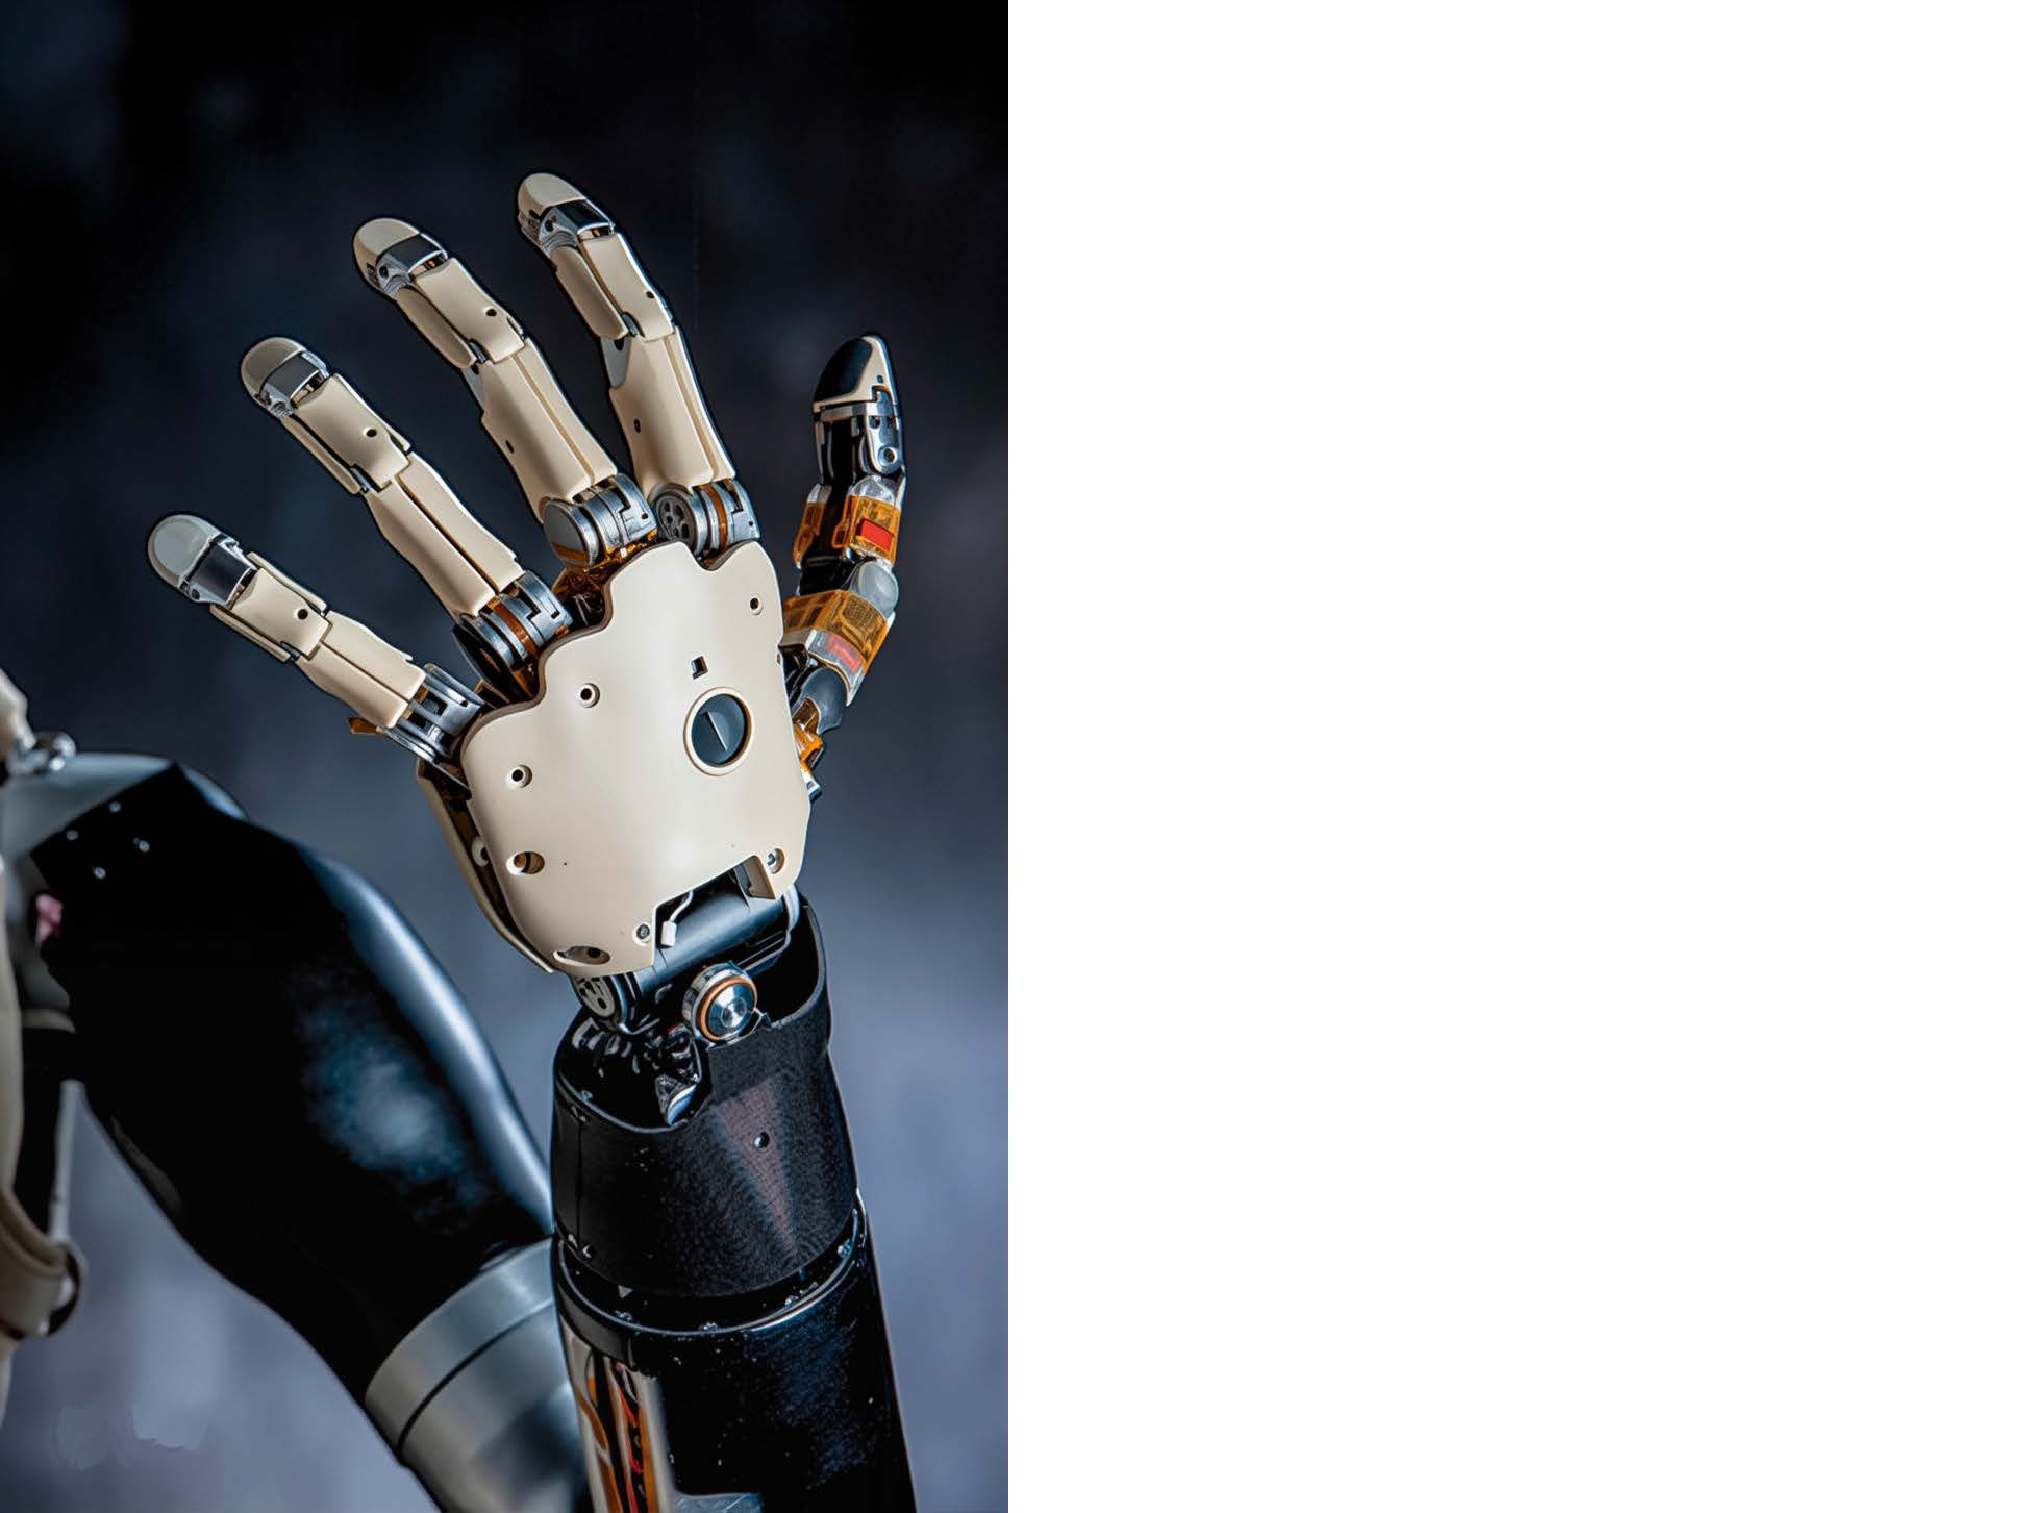
\includegraphics[width=0.5\linewidth]{chap1/1_5}
	\caption{功能强大的假肢如今触手可及。
		图片由约翰$\cdot$霍普金斯大学提供。 \label{fig:1_5}}
\end{figure}


生物力学甚至在科学领域之外也发挥着作用。电影制作人运用生物力学和动作捕捉技术,为游戏和电影创作计算机生成的图像,风格各异,从奇幻到逼真(图~\ref{fig:1_6})。
其成果将美感与科学的准确性完美结合,这在一两代人之前是难以想象的。


\begin{figure}[!htb]
	\centering
	\includegraphics[width=1.0\linewidth]{chap1/1_6}
	\caption{图片来自电影《阿凡达》和行为艺术家詹$\cdot$斯塔福德。
		她的动作被动作捕捉技术记录下来,并制作成计算机生成的图像。
		图片由二十世纪福克斯公司提供。 \label{fig:1_6}}
\end{figure}


总的来说,这些努力极大地改善了我们的生活。
现在,我们可以根据保持健康所需的日常体力活动水平获得建议,并且我们可以使用有助于我们实现健身目标的工具。
装配线、办公家具和许多消费品都符合人体工程学设计,以提高舒适度并防止受伤。
一些产品和程序已被设计用于置换髋关节和膝关节,减轻疼痛并恢复数百万骨关节炎患者的功能。
动力外骨骼正在彻底改变中风后康复,并可以使瘫痪患者恢复运动能力。
帕金森病等运动障碍已通过深部脑刺激得到成功治疗,深部脑刺激是指植入电极向大脑特定区域传递电脉冲。
硬膜外刺激是一种激活脊髓神经回路的技术,最近已显示出帮助脊髓损伤患者恢复自主运动的潜力。
运动员正受益于旨在降低受伤风险并提高运动表现的设备和训练计划(图~\ref{fig:1_7})。


\begin{figure}[!htb]
	\centering
	\includegraphics[width=0.6\linewidth]{chap1/1_7}
	\caption{生物力学研究有助于打造能够最大限度提升运动表现的运动器材。
		这款冰鞋的靴子和冰刀之间的铰链设计延长了冰刀与冰面的接触时间,从而增加了推进力的持续时间,从而提高了速度。
		图片由 McSmit 提供。 \label{fig:1_7}}
\end{figure}



\section{半机械人奥运会}


或许,更深入地观察一个引人注目的例子——“Cybathlon”(人机合体竞技),就能更好地理解生物力学的影响。
2016年,苏黎世联邦理工学院(ETH Zurich)教授罗伯特$\cdot$里纳(Robert Riener)组织了首届“Cybathlon”,这是一项将科学与体育进行创新性融合的运动。
与残奥会不同,这项运动的比赛项目侧重于日常任务。
例如,佩戴假肢的运动员比赛搬运物品、切面包、开罐子和晾衣服。
佩戴假肢的运动员比赛爬坡和上楼梯,同时保持杯子在碟子上保持平衡。
为了强调这项比赛关乎人类与科技的结合,参赛者被称为“飞行员”,而不是“运动员”。


在这场非传统的比赛中,最传统的体育项目是腿部瘫痪者自行车赛。
金牌被凯斯西储大学在罗纳德$\cdot$特里奥洛(Ronald Triolo)的科研领导下夺得。
该队的车手是马克·穆恩(Mark Muhn)(图~\ref{fig:1_8}),他在2008年的一次滑雪事故中脊髓受伤,胸部以下瘫痪。


\begin{figure}[!htb]
	\centering
	\includegraphics[width=0.6\linewidth]{chap1/1_8}
	\caption{马克$\cdot$穆恩参加 Cybathlon 比赛。
		图片由 Paul 和 Gabrielle Marasco 提供。 \label{fig:1_8}}
\end{figure}


凯斯西储大学的团队在功能性电刺激领域研究了四十年,并开发出了首批植入式神经肌肉刺激器。
特里奥洛相信,他们在植入电极方面的经验将成为制胜优势,因为其他团队正在使用通过皮肤传输电信号的电极。
植入电极可以更精准地刺激被激活的肌肉,从而产生更强烈的肌肉收缩。


该团队通过多种方式最大限度地提高了获胜的几率(McDaniel 等人,2017)。
他们购买了一辆卧式自行车,并将其拆解,去掉了所有不必要的重量。
他们让飞行员(最初有五名,其中两名被选中前往苏黎世)参加了强化训练计划。
我们最感兴趣的是他们使用的生物力学模型(图~\ref{fig:1_9})。


\begin{figure}[!htb]
	\centering
	\includegraphics[width=1.0\linewidth]{chap1/1_9}
	\caption{用于调整肌肉兴奋模式以产生循环的肌肉驱动生物力学模型的示例。 \label{fig:1_9}}
\end{figure}


特里奥洛表示,这些模型与我们在本书后面描述的类似,在两个方面发挥了作用:
首先,它消除了“死胡同”(行不通的想法);
其次,它优化了提供给飞行员的电刺激模式。
每块腿部肌肉的每一次收缩都由一个外部控制装置(一个绑在飞行员腰间的盒子)控制。
为了安全起见,飞行员可以控制盒子的开关。


为了获得刺激模式,研究小组从文献中获取了自行车运动的生物力学模型,并根据每位骑手的特点进行了定制。
定制非常重要,因为瘫痪后肌肉的特性会发生变化,而可以通过刺激激活的肌肉数量很少,所以适用于健全骑手的激活模式可能不适用于脊髓损伤患者的刺激驱动踩踏。
Musa Audu 带头为每位骑手建模和定制刺激模式,并采用第~\ref{chap:chap10}~章中描述的技术来估计每块肌肉激活的时间和强度。
值得注意的是,刺激模式在比赛期间从未改变。
当骑手的肌肉疲劳时,他的腿会保持以相同的速率抽动,但它们无法用那么大的力气推动,所以骑手必须换挡才能保持自行车前进。


事实上,飞行员之所以会很快感到疲劳,是因为功能性电刺激并不像大脑发出的自然信号那样募集肌肉纤维。
我们将在第~\ref{chap:chap4}~章中回顾这一现象,但现在只需说明,大多数自然发生的运动都是通过首先募集“慢肌”纤维(相对较小且抗疲劳),然后是“快肌”纤维(产生较大力量但很快疲劳)产生的。
然而,电刺激以相反的顺序募集肌肉纤维。
由于这种“反向募集”,飞行员在开始训练时几乎无法让摩托车持续行驶超过一分钟。



但意想不到的事情发生了——相比于单调乏味的固定自行车,飞行员们更喜爱比赛用自行车带来的户外锻炼。
而且运动训练可以增强瘫痪的肌肉。在飞行员们积极进取的激励下,经过5个月的训练,他们能够坚持骑车参加3分钟的比赛。
特里奥洛表示,他希望在未来几年找到一种技术解决方案来解决招募逆转问题,但在2016年,只有一个解决方案:“让我们的飞行员尽情锻炼”。
而且,这个方案真的奏效了!
在苏黎世,穆恩以2分58秒的成绩完成了750米的比赛,并夺得了金牌。


Cybathlon 的经历改变了 Muhn 的人生,或许更令人惊讶的是,它改变了 Triolo 的研究。
Triolo 说,以前他们的康复方法是任务导向的。
他们专注于让志愿者站立、行走或进行日常生活活动,比如穿衣和做饭。
但当他们的参与者在户外骑自行车,并开始在锻炼的同时享受乐趣时,一切都改变了。
他们锻炼得更多,这对他们康复的各个方面都产生了巨大的回报,包括提升了他们的自尊心。
当一名骑手在公共道路上骑自行车时,另一个骑手追上他并说:“轮子真漂亮。”
这几乎是陌生人第一次将他视为一个拥有酷炫自行车的人,而不是一个残疾人。



\section{研究运动的工具}

我写这本书的目标之一是让你熟悉我的团队和其他人员开发的肌肉驱动生物力学模型。重要的是要意识到这些模型是基于实验数据的。让我们来看看我们收集的数据类型。



分析运动的一种常用技术是在研究实验室和诊所录制个体的视频。
许多此类记录都是通过红外摄像机获得的,这些摄像机可以追踪贴在皮肤上的标记物,类似于电影制作中使用的技术(图~\ref{fig:1_10})。
最近,不需要标记物的运动捕捉技术变得越来越流行。
基于视频的系统已经广泛应用,但这些系统的普及程度已被惯性测量单元 (IMU) 所取代,IMU 现已集成到智能手机、可穿戴活动监测器和服装中。
IMU 能够在自然环境中长时间收集运动数据(速度和加速度),这对于监测病情进展和制定治疗方案非常有价值。
低成本活动监测器中 IMU 的普及也使得对全球数百万个体进行大规模研究成为可能(图~\ref{fig:1_11})。


\begin{figure}[!htb]
	\centering
	\includegraphics[width=1.0\linewidth]{chap1/1_10}
	\caption{前手翻(时长 2.9 秒)期间,贴在皮肤上的标记物轨迹。
		受试者最初站立(最左侧),然后向前跳跃,双手撑地翻身(中间),双脚落地,然后跳了一跳恢复平衡(最右侧)。
		球体间距越大,表示标记物移动速度越快。
		数据来自 ACCAD (2018)。 \label{fig:1_10}}
\end{figure}


\begin{figure}[!htb]
	\centering
	\includegraphics[width=1.0\linewidth]{chap1/1_11}
	\caption{717,527 名受试者超过 6800 万天的智能手机活动数据揭示了 111 个国家/地区的体力活动差异。
		图片改编自 Althoff 等人(2017 年)的研究,这是全球规模最大的体力活动调查。 \label{fig:1_11}}
\end{figure}


在实验室或诊所进行实验时,除了运动捕捉系统外,还可能涉及多种专用设备。
我们经常使用测力板来测量脚和地面之间的力。在步行和跑步研究中,使用跑步机很方便,因为受试者可以保持在运动捕捉系统能够精确测量的范围内。
一些跑步机还配备了测量地面反作用力的仪器。
肌电图用于测量各种肌肉活动的时间和强度。
我们可以监测跑步者的呼吸,测量消耗的氧气量和产生的二氧化碳量,以估算跑步所需的代谢能量。
磁共振成像和荧光透视成像等成像技术的普及使我们能够看到运动中的动物或人体内部,为可视化和测量运动提供了强有力的工具。


概念模型可以成为强大的分析工具,正如我们将在本书中看到的。
例如,第~\ref{chap:chap2}~章和第~\ref{chap:chap3}~章展示了一个简单的摆模型如何为我们合理地模拟行走,而一个质量弹簧模型如何为我们提供关于跑步的重要见解。
一个能够完成任务的简单模型几乎总是比一个更复杂的模型更受欢迎,后者提供了类似的实用性,但构建和理解起来更困难。
当然,并非所有复杂现象都能用简单的力学模型来表示。
正如我们将在第~\ref{chap:chap11}~章和第~\ref{chap:chap12}~章中看到的,肌肉驱动的模拟是强大的工具,可以填补第~\ref{chap:chap2}~章和第~\ref{chap:chap3}~章中简单模型所缺失的许多细节。


计算机模拟可以计算无法直接测量的量并预测假设场景中的运动,从而对实验进行补充。
模拟有助于理解例如难以通过实验研究的损伤。我们还可以估算导致观察到的运动的肌肉力量,以及关节负荷、肌腱应变和其他无法测量的量。
在正向动态模拟中,我们规定一块或多块肌肉的神经激活模式,然后预测肌肉骨骼模型的最终运动(图~\ref{fig:1_12})。
需要实验数据来开发和测试用于运动模拟的肌肉骨骼动力学数学模型,并评估模拟反映现实的程度。


\begin{figure}[!htb]
	\centering
	\includegraphics[width=1.0\linewidth]{chap1/1_12}
	\caption{典型的正向动态模拟的要素。
		运动源于神经、肌肉、骨骼和感觉系统的复杂协调。
		这些系统的计算模型使我们能够预测和分析人类和动物的运动。 \label{fig:1_12}}
\end{figure}


当我们测量了测试对象的运动并希望将这些数据转化为有意义的见解时,通常会使用逆过程,例如,肌肉必须产生哪些力才能产生测量到的运动。
为此,我们需要进行逆动力学分析,这是一种将实验数据与肌肉骨骼模型相结合的常见分析策略。
第一步是使用身体的生物力学模型,将标记位置的测量值(如图~\ref{fig:1_10}~所示)通过称为逆运动学的过程转换为关节角度(图~\ref{fig:1_13})。
关节角度根据时间进行微分,以估计关节角速度和加速度,然后将其与施加于身体的外力测量值结合使用,以估计关节力矩。
然后,将生物力学模型与优化算法结合使用,以估计肌肉力量。
我们将这种策略称为逆分析,因为运动测量值可用于推断产生这些运动必须存在哪些力。


\begin{figure}[!htb]
	\centering
	\includegraphics[width=1.0\linewidth]{chap1/1_13}
	\caption{典型逆动力学分析的要素。
		分析从测量标记轨迹和外力(右)开始,并使用生物力学模型估算身体各节段和关节的角度、速度和加速度。
		逆动力学模型和优化程序可估算关节力矩和肌肉力量。 \label{fig:1_13}}
\end{figure}




\section{本书概述}

在接下来的章节中,我们将首先使用简单的概念模型研究人类两种常见的运动形式——行走和跑步。
然后,我们将通过研究骨骼肌的生物学和结构、其与肌腱的动态相互作用以及肌肉如何产生驱动骨骼的力量来探索运动的产生。
接下来,我们将研究用于分析运动的模型和算法。
我们将演示如何从运动捕捉数据和生物力学模型中计算关节角度、关节力矩​​和单个肌肉的力量。
最后,我们将综合这些概念来研究肌肉在行走和跑步过程中的作用,并就我对该领域未来发展方向的一些看法进行总结。
如图~\ref{fig:1_14}~所示,本书的内容被安排成四个部分,我鼓励读者以这种方式来理解本书。
因此,第~\ref{chap:chap4}~章(第二部分的开头)并非第~\ref{chap:chap3}~章的续篇,但第~\ref{chap:chap5}~章无疑延续了第~\ref{chap:chap4}~章的篇幅。
如果您记住这一点,本书的内容将对您更有意义。


\begin{figure}[!htb]
	\centering
	\includegraphics[width=1.0\linewidth]{chap1/1_14}
	\caption{本书的组织结构。 \label{fig:1_14}}
\end{figure}



虽然我们主要关注人类的运动,但我们所描述的基本概念也可用于理解动物和机器人的运动。
本书涵盖的内容将帮助您理解精彩纷呈、内容丰富的科学文献,这些文献对众多主题进行了详尽的分析,而一本书根本无法涵盖所有​​这些主题。


\section{运动语言}

我想解释一下你需要了解哪些知识才能充分利用本书。
汤姆和我为熟悉某些工程基础知识的读者编写了本书。
数学和力学为分析运动提供了精确的框架,我们假设读者对向量和矩阵有基本的了解。
我们进一步假设读者熟悉自由体运动图、推导运动方程以及如何求解简单系统的运动方程。
如果你不熟悉这些主题,你应该准备好在遇到它们时花一些额外的时间去学习。


在生物学方面,了解人体解剖学和生理学背景会有所帮助,但并非必需。
对于不熟悉解剖学的读者,以下图表展示了本书将要用到的术语。这些术语包括解剖平面和方向(图~\ref{fig:1_15})、关节运动(图~\ref{fig:1_16}~和图~\ref{fig:1_17})以及主要骨骼和肌肉(图~\ref{fig:1_18}~和图~\ref{fig:1_19})。
这些术语乍一看可能令人望而生畏,但花几分钟时间研究这些图表并学习这些术语,对你大有裨益。


\begin{figure}[!htb]
	\centering
	\includegraphics[width=1.0\linewidth]{chap1/1_15}
	\caption{人体的解剖平面和方向。 \label{fig:1_15}}
\end{figure}


\begin{figure}[!htb]
	\centering
	\includegraphics[width=1.0\linewidth]{chap1/1_16}
	\caption{肩部、肘部、骨盆和臀部在额状面(左)、矢状面(中)和横状面(右)的运动。 \label{fig:1_16}}
\end{figure}


\begin{figure}[!htb]
	\centering
	\includegraphics[width=0.75\linewidth]{chap1/1_17}
	\caption{膝盖和脚踝在矢状面上的运动。 \label{fig:1_17}}
\end{figure}


\begin{figure}[!htb]
	\centering
	\includegraphics[width=0.95\linewidth]{chap1/1_18}
	\caption{人体下肢的主要骨骼、解剖标志和肌肉(前视图)。 \label{fig:1_18}}
\end{figure}


\begin{figure}[!htb]
	\centering
	\includegraphics[width=0.75\linewidth]{chap1/1_19}
	\caption{人体下肢的身体部分和主要肌肉(后视图)。 \label{fig:1_19}}
\end{figure}


这本书只是我的一个开端,我希望它能成为你持续探索的旅程。
我们的梦想是,你能在此汇集的素材基础上,迸发出你独特的创造力火花,探索自然,创造一些能够丰富他人生活的东西。

















\chapter{行走} \label{chap:chap2}

\begin{figure}[!htb]
	\centering
	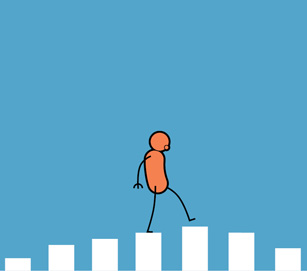
\includegraphics[width=0.5\linewidth]{chap2/2_0}
	% 加星号(*)表示不加编号
	\caption*{ \label{fig:2_0}}
\end{figure}

每走一步,你都会向前倾斜一点点,然后站稳,避免摔倒,一遍又一遍,你都在摔倒,然后站稳,避免摔倒。

\begin{flushright}
	——劳里·安德森 \\
\end{flushright}

\begin{figure}[!htb]
	\centering
	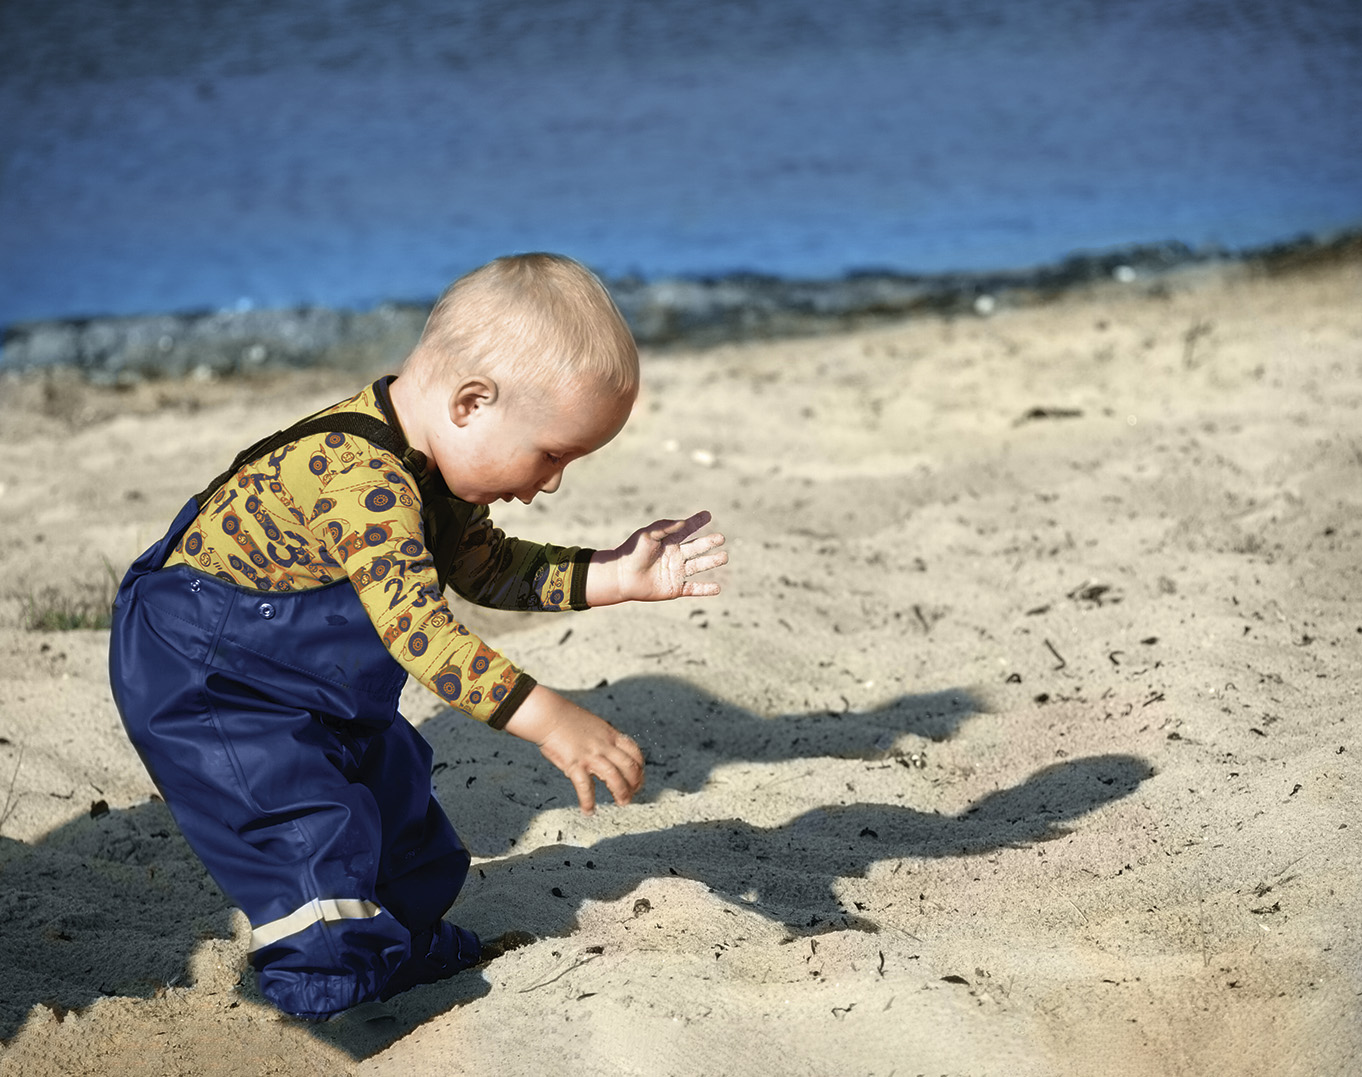
\includegraphics[width=0.5\linewidth]{chap2/2_0_2}
	% 加星号(*)表示不加编号
	\caption*{ \label{fig:2_0_2}}
\end{figure}

“有一天,我在月球上漫步,”
宇航员哈里森$\cdot$施密特兴高采烈地唱着,他即将踏上最后一次阿波罗任务的首次月球行走。
“在快乐的五月,”指挥官吉恩$\cdot$塞尔南附和道。
一缕缕月尘从他们的靴子上溅起,他们……究竟在做什么?跳跃?腾跃?跌跌撞撞?……穿过月球表面。


不管它是什么,它与我们通常认为的行走几乎没有什么相似之处。
施密特像个蹒跚学步的孩子一样慢步走着,左右摇晃。
塞尔南的步态看起来像个孩子骑着扫帚,却假装那是一匹马。
这两位训练有素的宇航员仿佛忘记了人类最基本的技能——行走——不得不学习一种新的移动方式(图~\ref{fig:2_1})。


\begin{figure}[!htb]
	\centering
	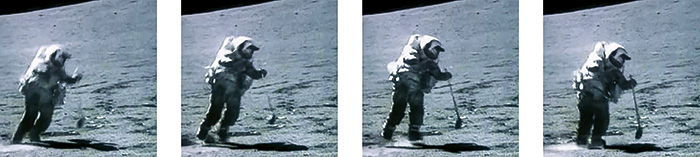
\includegraphics[width=1.0\linewidth]{chap2/2_1}
	\caption{宇航员很少在月球表面“行走”,他们更喜欢在月球引力下跳跃行走。
		图片由NASA提供。 \label{fig:2_1}}
\end{figure}


在本章中,我们将探讨为何看似简单的行走——人类进化已完美适应地球引力——在月球上却变得如此困难。
宇航员奇特的步态或许能帮助我们更充分地理解行走过程中发生的一系列精心安排的事件,以及引力在其中扮演的关键角色。


欣赏行走壮举的另一种方式是建造一台能够行走的机器。
塔德$\cdot$麦吉尔(Tad McGeer)的巧妙实验表明,一个拥有类似人类比例的无动力装置可以在倾斜的表面上行走。
这些装置无需大脑、脊髓或肌肉即可行走,只需在正确的方向上轻轻推一下即可。
这一观察表明,我们可以通过简单的机械模型来深入了解行走,我们将在本章中对此进行演示。


然而,在开始分析之前,有必要先了解一下步态周期以及运动中涉及的一些基本物理知识。
下一节将为你提供一些正确的方向。


\section{步行步态周期}

人类有两种常见的步态:行走和跑步。
我们都熟悉身体各部分在行走时所经历的典型周期性模式,但更正式地描述这些定性观察结果会很有帮助。
一个行走步态周期由同一条腿上连续两次的足部接触事件界定,另一条腿的足部接触通常发生在中途(图~\ref{fig:2_2})。
每条腿都有一个支撑期(此时足部接触地面)和一个摆动期(此时足部离地)。
支撑期始于足部接触地面,结束于足尖离地,对于一条腿而言,它占行走步态周期的约 60\%;其余时间则用于摆动。
由于支撑期比摆动期长,因此在每个行走步态周期中,都有双脚接触地面的时期,我们称之为双支撑期。
我们将只有一只脚接触地面的间隔称为单支撑期。


\begin{figure}[!htb]
	\centering
	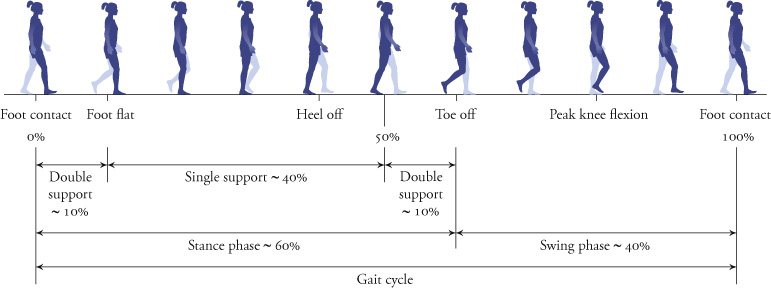
\includegraphics[width=1.0\linewidth]{chap2/2_2}
	\caption{步行步态周期及其组成事件(例如,脚接触)和阶段(例如,双支撑)。 \label{fig:2_2}}
\end{figure}


步长是指两个连续足迹上同一点之间沿行进线的距离(图~\ref{fig:2_3})。
连续两步所走的距离,或一个步态周期所走过的距离,称为步长。足部接触事件发生的速率(相当于步长持续时间的倒数)称为步频或步频;
迈步的速率称为步频。
步行速度可以用步长与步频的乘积来计算,或者也可以用步长与步频的乘积来计算:


\begin{figure}[!htb]
	\centering
	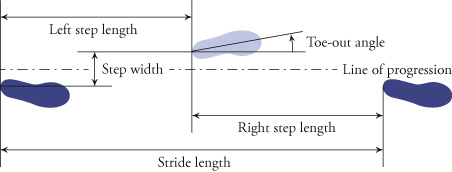
\includegraphics[width=0.8\linewidth]{chap2/2_3}
	\caption{水平(地面)平面上的步态测量。 \label{fig:2_3}}
\end{figure}

\begin{equation}
	\text{速度} = \text{步长} \times \text{步频}
			    = \text{步长} \times \text{起落}
\end{equation}

个人通常的步行速度会因身高、体能和其他因素而异。
健康成年人在平地上通常选择以约1.2-1.4米/秒的速度行走,步频为2步/秒。
典型的步长约为0.6-0.7米。


另外两个值得注意的指标是在水平面上测量的(图~\ref{fig:2_3})。
步宽是脚平放时脚后跟中点与另一条腿上相同点之间的距离,垂直于进展线测量。健康成年人的步宽约为腿长的 10\%。
如果腿长约为 1 米,步宽约为 10 厘米,但对于正在学习走路的幼儿和一些平衡能力较差的人来说,步宽会更大。
足部进展角是进展线与连接脚后跟中点和第二个脚趾(即足部的长轴)的线之间的角度。
正和负的足部进展角分别称为外倾角和内倾角。
成年人的外倾度通常较小,约为 10 度,但这个值在患有肌肉骨骼或神经系统疾病的个体之间可能会有所不同。
例如,患有小脑性共济失调(会导致平衡障碍)的人可能会以更大的脚趾向外和步宽行走,以减少跌倒的风险。


\section{地面反作用力}

我们通过测量双脚与地面之间的力来研究行走(图~\ref{fig:2_4})。
我们将在第~\ref{chap:chap11}~章中学习更多关于行走过程中肌肉协调的知识;
目前,只需知道肌肉通过产生力来产生运动即可。
肌肉产生的“作用力”会导致地面对双脚施加“反作用力”。
行走过程中,可以使用测力板测量地面反作用力。
测力板是一种仪器,可以测量人在测力板上行走时在垂直方向、前后方向和左右方向受到的力。​​
地面反作用力很重要,因为它可以衡量身体重心在每个时刻的加速度。
我们可以使用牛顿第二定律将地面反作用力和其他外力与身体重心 (com) 的加速度联系起来:
\begin{equation}
	F_{\text{external}} - mg = m a_{\text{com}} \label{eq:2_2}
\end{equation}
其中 $F_{external}$ 是施加于身体的所有外力之和,$m$ 是身体的总质量,$g$ 是重力加速度,$a_{com}$ 是质心加速度。
值得花点时间思考一下上一句中“和”和“全部”这两个词的含义。
当双脚接触地面时,我们必须将施加于每只脚的力相加。由于公式~\ref{eq:2_2}~是矢量和,所以方向很重要。
双脚下方力的垂直分量支撑着身体的重量。
但是,正如您在图~\ref{fig:2_5}~中所看到的,前脚上的前后力往往会抵消后脚上的前后力;
也就是说,前脚充当了刹车的作用,阻止我们走得越来越快,而后脚则提供推进力。
如果没有施加外力(即 $F_{external} = 0$,则物体处于自由落体状态,其质心将以 $g = 9.81 m/s^2$ 的速度加速向地面坠落。



\begin{figure}[!htb]
	\centering
	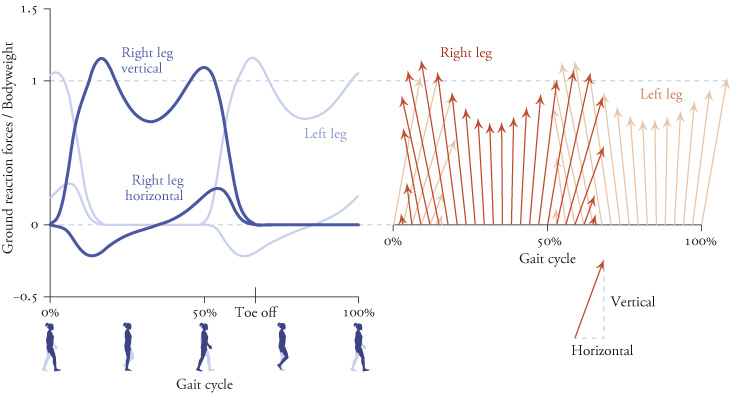
\includegraphics[width=1.0\linewidth]{chap2/2_4}
	\caption{以 1.55 米/秒的速度行走时代表性的地面反作用力。
		图中显示了步态周期内的垂直和水平(前后)分量(左)以及总矢量示意图(右)。
		正水平力指向前方。
		较小的左右力未显示。
		数据来自 Dembia 等人(2017)。 \label{fig:2_4}}
\end{figure}


\begin{figure}[!htb]
	\centering
	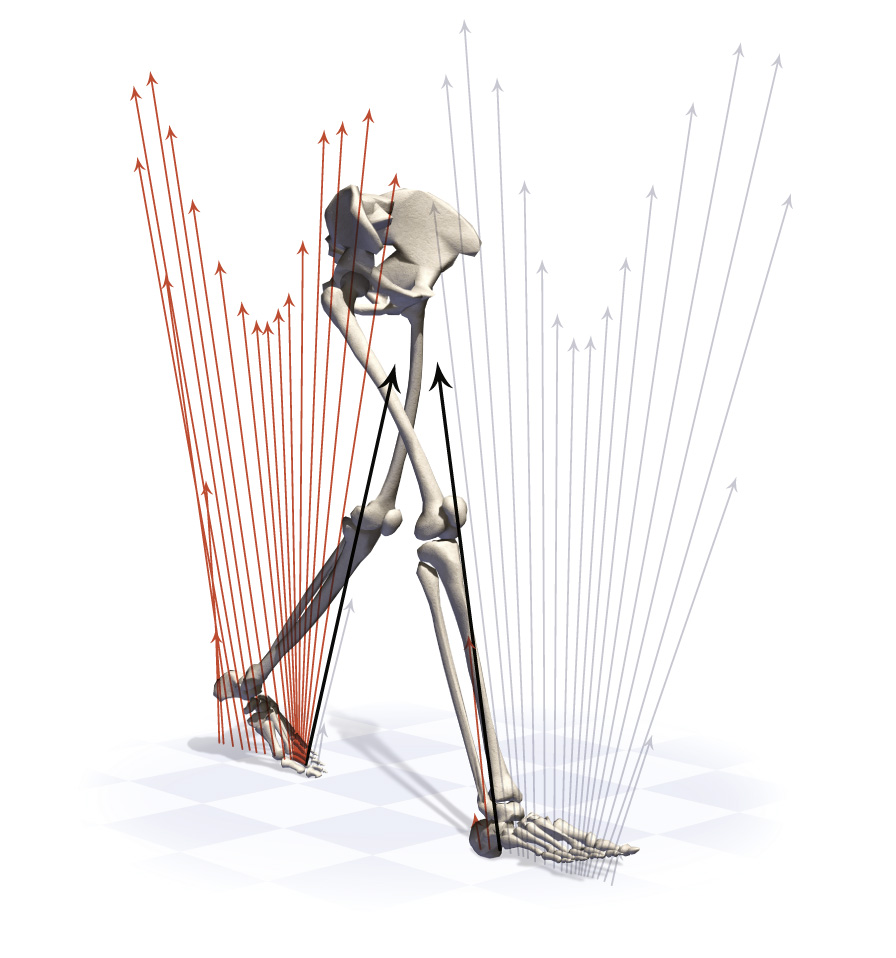
\includegraphics[width=0.9\linewidth]{chap2/2_5}
	\caption{以 1.55 米/秒的速度行走时,用两块测力板测量地面反作用力。
		两组箭头表示每只脚随时间推移受到的力。​​
		如黑色箭头所示,在双脚支撑时,地面反作用力的前后分量指向相反的方向。 \label{fig:2_5}}
\end{figure}


行走过程中地面反作用力的记录显示出几个有趣的特征(图~\ref{fig:2_6})。
地面反作用力的垂直分量在足部接触地面后迅速上升,并在步态周期的约 10\% 处达到大于体重的力。
在站立中期,垂直力降至低于体重,然后在蹬地时再次上升至高于体重。
然后,垂直力降至零,因为在脚趾离地后,足部不再接触地面。
平均而言,总垂直地面反作用力等于体重的 1 倍。
请注意,根据公式~\ref{eq:2_2},当地面反作用力的垂直分量等于体重时,重心没有净垂直加速度,恰好平衡了重力产生的向下力。

\begin{figure}[!htb]
	\centering
	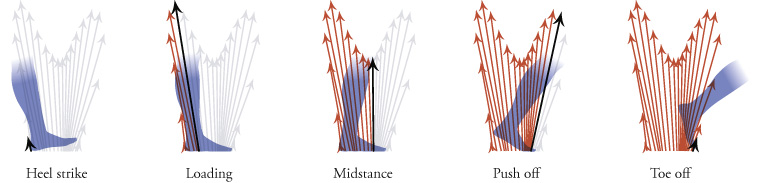
\includegraphics[width=1.0\linewidth]{chap2/2_6}
	\caption{以 1.55 米/秒的速度行走时,足部受到的典型地面反作用力。
		此处显示的力矢量(在空间中)与图~\ref{fig:2_4}~中显示的力矢量(随时间变化)相同。 \label{fig:2_6}}
\end{figure}


在站立的前半段,水平地面反作用力指向身体后部,使重心减速,之后指向身体前部。
除了图~\ref{fig:2_4}~所示的前后分量外,水平地面反作用力还有一个内外分量,这个分量虽然很小,但对于控制左右平衡很重要。
虽然在任何特定时刻重心都可能加速,但在几步匀速行走中,平均前后加速度为零。
改变前进速度时,平均前后加速度将不为零。
在垂直方向上,改变坡度时会出现非零平均加速度,例如从平地走到斜坡上时。


请记住,在步态周期的某些阶段,双脚都会接触地面,两个力相加,形成作用于身体的净向上力(图~\ref{fig:2_5})。
一个地面反作用力指向上方和前方,另一个指向上方和后方。
净地面反作用力主要指向上方,在双脚支撑阶段开始时有一个较小的向前分量,在脚趾离地时有一个较小的向后分量。
这些力抵消了向下的重力,并帮助您调节步行速度。


可以将测力板记录除以身体总质量,以估算质心加速度(公式~\ref{eq:2_2}~中的 $a_{com}$)。
该加速度可以积分一次以估算质心速度 ($v_{\text{com}}$),积分两次以估算其位置 ($r_{com}$)。
根据这些量,可以估算出质心向前的动能 ($E_{kf}$),其公式如下:
\begin{equation}
	E_{kf} = \frac{1}{2} m v_{\text{com}}
		   = \frac{1}{2} m 
		   	 ( \int a_{\text{com},f} (t) dt )^2  \label{eq:2_3}
\end{equation}
%
其中“$f$”下标表示前向分量
(请注意,垂直方向的速度波动非常小,因此我们在此忽略它)。
公式~\ref{fig:2_3}~中的积分符号提醒我们,加速度的影响是累积的,如果我们想要知道速度或动能,就必须将其随时间积分。
前向动能在站立中期最低,因为在站立的前半段,水平地面反作用力向后,使重心减速。
重力势能可以估算为:
\begin{equation}
	E_{\text{pg}} 
		= m g r_{\text{com},\text{v}} \label{eq:2_4}
\end{equation}
%
其中“v”下标表示垂直分量。
重力势能在站立中期达到最高,此时身体跨过站立肢(图 2.7)。
如果我们绘制步态周期中的前向动能和重力势能,我们会发现它们是异相的(图 2.8):
当重力势能接近最小值时,前向动能达到峰值,反之亦然。
因此,总能量几乎保持不变。
我们在行走过程中保存能量的方法之一是用重力势能换取前向动能或前向速度,类似于在重力影响下摆动的钟摆的情况。
这一观察结果表明重力与行走有很大关系。


\section{弹道步行模型}

1980年,托马斯·麦克马洪(Thomas McMahon)和西蒙$\cdot$莫雄(Simon Mochon)基于以下假设,开发了一个行走数学模型:身体将势能转化为动能,并最大限度地减少肌肉在摆动阶段的作用。
该模型非常简单,仅由三个刚性连杆和三个旋转(销)关节组成,值得注意的是,没有肌肉或运动(图2.9)。
支撑肢由一个倒立摆表示,该摆的踝关节固定在地面上,使肢体能够在矢状面上绕踝关节旋转;
支撑肢的膝盖被假设锁定在完全伸展的位置。
摆动肢被建模为一个双摆,大腿和小腿部分在膝盖处通过销连接。
两条腿在臀部处固定在一起,并具有真实的质量分布。
头部、手臂和躯干的质量被忽略,但它们的质量集中在臀部。


肌肉活动的实验记录表明,在正常速度行走过程中,除了在摆动期的开始和结束时,摆动肢的肌肉相对不活跃。
因此,弹道步行模型假设肌肉完全被动地确定模型启动和完成摆动期所需的肢体节段的位置和速度,仅受重力作用(就像抛射物,因此称为“弹道”)。
当肌肉不活跃时,摆动肢的行为被认为类似于非受迫双摆。
如果在脚趾离地时为模型提供恰到好处的初始条件,则摆动肢的脚趾将在摆动中期离开地面,并且膝盖将在脚接触时完全伸展。


\section{弗鲁德数}

倒立摆本身是一个比弹道行走模型更简单的模型,它无法准确预测人类的步行速度,但确实提供了一些关于人类步行速度的物理限制的重要见解。
考虑一个倒立摆,如图 2.9 左侧所示,长度为 $l$,体重 $m$ 集中在臀部。
当臀部处于最大高度时,其瞬时速度 $v$ 水平方向,踝关节的垂直反作用力 ($F$) 等于向心力:
%
\begin{equation}
	F = \frac{m v^2}{l}
\end{equation}
% 
向心力是必须施加在摆锤上,以防止其离开地面的向下力。
由于地面无法对脚施加向下的力(除非你踩到胶水),所以向心力必须由体重 $mg$ 产生。
将这些力相等,并解出速度,我们发现倒立摆模型的最大行走速度 ($v_{max}$) 为
%
\begin{equation}
	v_{\text{max}} = \sqrt{g l}
\end{equation}

我们用$v_{max}$来定义无量纲步行速度($v^{*}$):
\begin{equation}
	v_{*} = \frac{v}{v_{max}}
\end{equation}
%
当速度超过 $v_{max}$ 时,脚会离开地面;因此,$0 \leq v^{*} \leq 1$,此时我们行走时就像一个倒立摆。
弗劳德数 ($F_r$) 是一个无量纲量,表示向心力与重力之间的比率:
%
\begin{equation}
	F_r = \frac{v^2}{g l}
		= (v^{*})^2
\end{equation}
%
无量纲步行速度和弗劳德数为比较不同最大速度和腿长的动物和人的步行速度提供了非常有用的指标。


倒立摆模型的一个重要预测是,如果 $l$ 或 $g$ 减小,最大步行速度也会减小。
当观察一个孩子与一个成年人并肩行走时,第一个关系很明显。
由于腿较短,孩子的弗劳德数会比成年人高,因此 $v_{max}$ 会较低。
因此,您可能会观察到成年人以舒适的速度行走,而孩子则跑着跟上。 
$v_{max}$ 对重力 $g$ 的依赖性解释了宇航员在月球表面遇到的挑战。
由于月球上的重力仅为地球的六分之一左右,因此月球上的 $v_{max}$ 与地面上的值相同。
因此,正常的地球步行速度会导致宇航员离开月球表面。
因此,阿波罗 11 号宇航员尼尔$\cdot$阿姆斯特朗和巴兹$\cdot$奥尔德林大多以慢速行走,以保持双脚着地。
后来的宇航员采用了各种各样的跳跃步态。
有趣的是,登月任务前的实验表明,袋鼠跳是最有效的步态,但宇航员很少采用这种策略。



值得注意的是,人类和其他陆地动物通常不会在弗劳德数为 1 时行走;
它们会在弗劳德数约为 0.5 时从行走过渡到奔跑以节省能量。
一个重要的例外是大象,它是最大的陆地动物,当弗劳德数大于 1 时,它们的行走速度似乎比倒立摆模型允许的速度快得多 (Hutchinson 等人,2003)。
与往常一样,理论与观察之间的差异提供了学习的机会。
从 2003 年到 2010 年,John Hutchinson 及其同事研究了视频,并使用定制的测力板对大象进行了实验。
(它们必须是强大的测力板!)
Hutchinson 发现,尽管大象始终至少有一只脚着地,因此仍然是传统意义上的“行走”,但它在高速下会夸张地蹲下(图 2.10)。
这种“格劳乔步态”以喜剧演员格劳乔$\cdot$马克斯(Groucho Marx)的名字命名,他推广了这种行走方式。
这种步态意味着腿部肌肉产生巨大的力量,重力势能和动能的交换与倒立摆行走模型不一致。
因此,大象的步态某种程度上是行走和跑步的混合体。
下一章将讨论行走和跑步的区别,以及另一种大型动物——霸王龙——是否能够奔跑,届时我们将更详细地解释这一概念。


\section{运输成本}

弹道步行模型捕捉到了正常步行的一些显著特征,部分原因是我们自然而然地学会了如何以最小化能量消耗的方式移动。
减少腿部摆动时的肌肉活动就是一个例子。
我们也会自然地选择步行速度、节奏、步宽和其他变量,以最小化传输成本或移动给定距离所需的能量(图 2.11)。
过去 60 年来的许多研究已经证实,我们行走的方式可以最小化传输成本——这是生物力学的一个重要原则。
步行的传输成本通常是通过收集和分析一个人以特定速度行走时吸入和呼出的混合气体来估算的(图 2.12)。


请注意,我们无法直接测量能量消耗,但基于呼吸测量的间接估算是一个很好的替代方法。
我们的肌肉由燃烧碳水化合物、脂肪和蛋白质的化学反应提供动力。
这些反应消耗氧气并产生二氧化碳。通过确定废气产生的速率,我们可以推断出使用了多少燃料,从而消耗了多少能量。
如图 2.11 所示,我们通常将运输成本表示为每公斤体重移动一米所需的焦耳能量。



虽然弹道模型有助于理解行走的一些基本特征,但它也存在一些局限性。
例如,它无法模拟双支撑,而这对于理解连续步伐之间的过渡至关重要。
倒立摆模型预测我们的最大行走速度将发生在弗劳德数为 1 时,而实际上人类在弗劳德数远低于 1 时从行走过渡到跑步,竞走运动员在弗劳德数大于 1 时可以“行走”。
还要注意,弹道步行模型可能会让人得出结论,认为行走不会消耗任何能量。
此外,具有刚性站立肢的模型无法准确预测实验观察到的地面反作用力。
最后,弹道步行模型不会产生重复的步态周期。
其中一些限制在一个稍微复杂一些的模型(称为动态步行模型)中得到了解决。


\section{动态步行模型}

弹道行走模型在钟摆模型的基础上,通过增加膝盖(或者更准确地说,一个膝盖)进行了改进。
我们或许会认为,再增加一个解剖学元素就能进一步改进模型。
但它的作用远不止于此:
通过增加双脚,塔德$\cdot$麦吉尔设计了一个可以在实验室中制造和测试的行走机器人。


麦吉尔曾接受过航空工程师的培训,因此他采用的策略与一个世纪前飞机研发的策略如出一辙也就不足为奇了。
在尝试动力飞行之前,莱特兄弟多年来一直致力于研发利用滑翔机下坡时重力势能驱动的滑翔机。
到1902年底,他们已经完成了数百次此类飞行。
莱特兄弟掌握了滑翔技术后,便自信满满地掌握了动力飞行,并于次年完成了首次动力飞行记录(Collins 等人,2005)。


效仿莱特兄弟,在莫雄和麦克马洪提出弹道模型十年后,麦克吉尔构建了一种被动机构,在适当的初始条件下,该机构可以仅靠重力驱动,稳定地从缓坡上行走(图 2.13)。
证明这种机构的可构建性是一项突破,并开启了“动态行走”研究的新领域,动态行走主要由腿部的被动动力学产生运动。
如今,动力驱动的动态步行机器人的设计遵循莱特兄弟的原理:
如果被动机构能够严格在重力作用下从缓坡上移动,那么主动机构应该能够使用执行器在平地上移动,执行器仅注入重力在下缓坡时提供的少量能量。



动态步行模型在三个关键方面扩展了弹道模型:添加双脚、建模双支撑,以及最重要的,实现一步一步的过渡(图 2.14)。
这些特性使该机构能够进行周期性、连续的步行。
在单支撑期间,支撑肢的脚在地面上滚动(不滑动),而摆动肢被动摆动。
膝关节伸展止动装置可防止摆动结束时膝关节过度伸展,并保持支撑肢完全伸展,被动支撑身体重量。
在支撑的前半段,重心向上移动,在后半段向下移动。
就在脚接触之前,支撑肢踝部产生的推离力矩将重心重新定向到向上的轨迹。
在脚接触之前重新定向重心可降低脚与地面碰撞的速度和相应的能量损失。
在脚与地面碰撞时以及膝盖完全伸展时撞到止动装置时,仍然会损失一些能量。
为了实现连续的步态,每一步都必须注入少量能量,以补偿能量的耗散以及关节的摩擦损失。
在完全被动的步行机中,这种能量由行走机构在缓坡下行时产生的重力势能提供;
在平地上,这种能量可以由位于踝部或臀部的电机注入。


动态步行模型为理解平地行走的一些基本特征提供了一个理论框架。
动态步行模型已用于研究步态周期中的能量消耗、能量消耗如何随步行速度而变化以及人类步行的其他方面。
例如,在开始双脚支撑时改变质心轨迹所需的能量称为步进转换成本。
动态步行模型正确地预测了该成本会随着步幅更大、速度更快而增加。
增加步长(同时保持步频恒定)会增加能量消耗,因为质心速度增加,其轨迹必须改变更大的幅度。
增加步频(同时保持步长恒定)也会增加能量消耗,因为腿部必须比单独由被动动力学产生的速度更快地摆动,而肌肉会消耗能量来摆动腿部。


步步过渡和腿部强制摆动运动所产生的能量消耗,除了维持平衡外,还会影响人类行走的成本。
人类通常会选择步长和步频,以最小化运输成本。
当步行速度超过运输成本最低的速度时,人类会以几乎等比例增加步长和步频,以平衡步步过渡和腿部强制摆动带来的成本增加。
步步过渡的成本也可以通过将我们的双脚像轮子的一部分一样使用(请注意图 2.14 下方的弧形双脚)来降低,从而减少所需的重心方向变化。
当地面反作用力从脚接触时的后脚掌转移到脚趾离地时的前脚掌时(图 2.5),人类的双脚实际上在地面上滚动。
对于动态步行者来说,脚的位置至关重要:
如果脚的位置过于前倾,步行者就会向后摔倒;
如果腿部摆动速度过慢且步长过短,步行者就会向前摔倒。


动态步行模型比弹道模型具有更强的分析能力,但当然也存在局限性。
许多建模假设和简化使得该模型无法用于研究人类步行的某些要素。
例如,动态步行模型假设运动严格为平面运动,忽略了矢状面以外的运动。
McGeer 的装置通过将腿部数量增加一倍来最大限度地减少左右摇摆,从而强化了这一假设。
2001 年,当时就读于康奈尔大学的史蒂夫·柯林斯 (Steve Collins) 制造了第一台双足被动动态步行机(图 2.15)。
设计这种机制需要仔细关注机器质心的轨迹,以防止其因非矢状面运动而跌倒。
矢状面上的反向摆动臂稳定了偏航,足部形状和侧向摆动臂控制了倾斜,而柔软的鞋跟则避免了对足部接触时姿势的敏感性(Collins 等人,2001)。
在每种情况下,仿生学都改善了机制的性能,并且让我们了解了为什么这些要素(手臂摆动、脚和脚跟)会给人类带来生物力学优势。


\section{手臂摆动}

到目前为止,我们已经使用了简单的模型来研究下肢的动力学,但上肢在行走中也发挥着作用。
上肢最明显的运动是手臂摆动,但我们行走时为什么摆动手臂却不那么明显。
为了研究这种行为,史蒂夫$\cdot$柯林斯和他的同事提出了一种类似于麦吉尔的直腿被动行走机制,但在臀部连接了一个类似手臂的摆锤(图 2.16)。
他们测试了几种手臂摆动策略,包括我们熟悉的“正常”摆动,以及一种“反正常”摆动,即左臂随左腿前进,右臂随右腿前进。
我不禁将这种策略称为“兄弟步”,以纪念我的哥哥布莱恩$\cdot$德尔普,他小时候喜欢这样走路,我们俩都喜欢。


对正常行走的人类受试者进行的实验表明,肩关节和肘关节肌肉的活性较低,这证实了正常的手臂摆动主要是被动的。
下肢的运动学和动力学不受手臂摆动策略的影响,但当手臂不摆动时,整个身体会绕垂直轴旋转得更大,而在反常手臂摆动时,旋转幅度更大。
角动量的增加被绕垂直轴更高的地面反作用力矩所抵消,从而导致肌肉活性和能量消耗相应增加。
简而言之,Bro步法很不协调,这就是为什么超过一定年龄的人通常不会这样走路。


\section{用于步态分析的骨骼模型}

由于被动步行器的每个仿生特征都提升了其性能,人们自然会好奇一个更高保真度的模型会是什么样子。
让我们先来听听一些坏消息:
解剖关节非常复杂,相邻的身体部位会在各个方向上相对平移和旋转。
我们通常只关注这些运动中的一小部分,或者只能精确测量它们。
因此,即使是刻意模仿人体的模型也会做出一些简化的假设,例如不允许股骨头和骨盆之间的相对平移,从而将髋关节表示为球窝关节。


尽管如此,图 2.17 展示了一个用于分析步态的典型且相当准确的下肢骨骼模型。(必要时可添加躯干和手臂。)
该模型由 9 个关节刚体组成:骨盆、左右股骨、髌骨、胫腓骨(小腿)和足部。
该模型的下肢有 16 个自由度:6 个自由度描述骨盆相对于固定参考系的位置和方向(倾斜、侧倾和旋转),5 个自由度描述每条腿的姿势(髋屈曲、内收和旋转;膝关节伸展;踝关节背屈)。
这些术语是标准术语,值得学习,如图 1.16 所示。


想一想:在我们行走的每一刻,我们都在不知不觉中同时控制着十几个角度位置。
相比之下,莫洪和麦克马洪的弹道行走模型只有3个自由度,动态行走模型也只有几个自由度。
我们之所以成功,部分原因在于我们走捷径,尽可能地使用被动运动,但也因为我们的大脑在生命的第一年花费了大量时间学习如何协调复杂的行走动作。
下次你再开玩笑说有人不能一边走路一边嚼口香糖时,请记住,即使是第一步——双足行走——也是一项了不起的成就。


请注意,图 2.17 所示的模型是三维的。
正如我们所见,行走是一种三维活动,必须分析非矢状面的运动和力才能理解平衡和体重支撑。
有多种方法可以测量这些三维运动,我们将在第 7 章中介绍。
我们可以使用这些方法来估计人类受试者在行走过程中的运动,我们将在下文中介绍。


\section{步行运动学}

行走时,骨盆会经历复杂的运动(图 2.18)。
在额状面上,由于肢体在站立初期负重,骨盆会向摆动侧向下倾斜。
该运动的范围几乎翻倍,从低速行走时的约 5 度增加到高速行走时的约 10 度。
在横切面上,骨盆向前进肢旋转;
因此,前肢的髋部位于后肢的髋部前方。
该运动也会随着速度的增加而增强,并提供了一种增加步长的机制。


下肢关节也以典型的模式运动(图2.19)。
足触地时,髋关节处于屈曲状态。
在站立期,髋关节伸展,在足尖离地前达到最大伸展度,然后在摆动期屈曲。
足触地时,膝关节完全伸展。
当肢体负重时,膝关节像减震器一样先屈曲后伸展,速度越快,屈曲度越大。
在摆动前,膝关节快速屈曲,在摆动中期附近达到最大屈曲度,然后快速伸展,在下一次足触地前达到完全伸展。
足触地时,踝关节处于中立位。
在站立初期,随着足部向地面旋转,踝关节跖屈;
当胫骨越过足部时,踝关节背屈。
在站立期接近尾声时,踝关节快速跖屈,大约在足尖离地时达到最大伸展度。
随着步行速度的增加,峰值关节角度通常会增加,而步态周期中站立的时间会减少。


\section{地面反作用力和步行速度}

图 2.20 显示了行走过程中的地面反作用力。
高速行走时,地面反作用力的垂直分量在足部触地后迅速上升,并呈现出特征性的双峰形状。
我们在图 2.4 至 2.6 中也看到了类似的形状。
随着速度的增加,这些峰会变得更加明显。
地面反作用力的第一个峰来自支撑身体重量的前肢肌肉。
地面反作用力的第二个峰来自蹬地时后肢肌肉。
这些反作用力有助于我们了解重心的加速度,但仅凭实验无法告诉我们哪些肌肉负责产生测量到的地面反作用力。
我们将在第~\ref{chap:chap11}~章中研究肌肉如何协调行走并产生地面反作用力。


图 2.18–2.20 所示的数据可从 simtk.org 免费下载。
此类规范数据对于量化受试者的步态偏差以及测试运动模型和模拟的准确性非常有价值。


\section{非典型步态}

人类可以利用本章讨论的机制平稳高效地行走。
然而,身体或大脑的损伤以及关节或肌肉的疾病可能会扰乱行走动力学。
例如,脑瘫患者(一种因脑损伤引起的运动障碍)经常以蹲伏步态行走(图 2.21)。
蹲伏步态的特点是站立期膝关节过度屈曲。
膝关节过度屈曲会带来问题,因为它会增加站立期膝关节的力量,阻碍摆动时脚趾与地面的间隙,并显著增加能量消耗(尝试以蹲伏步态行走两分钟,看看是否会气喘吁吁)。
脑瘫患者的膝关节过度屈曲通常会随着时间的推移而恶化,常常导致膝关节力学改变和慢性膝关节疼痛。
在严重的情况下,膝关节屈曲程度可能会变得非常严重,以至于患者完全丧失行走能力。


许多脑瘫患者以及中风患者行走时,都会出现膝关节僵硬的步态,即摆动期膝关节屈曲功能减弱且延迟(图 2.22)。
这种步态还会降低脚趾与地面的距离,导致绊倒或需要进行能量效率低下的代偿性运动。
膝关节僵硬的步态被认为主要是由股直肌活动不当引起的,股直肌经髌骨穿过膝关节前方,产生膝关节伸展力矩。
因此,膝关节僵硬的步态通常采用股直肌转移术治疗,将股直肌的附着点从髌骨转移到一个能够降低其产生膝关节伸展力矩能力的部位。
遗憾的是,股直肌转移术的结果并不一致:
有些人在手术后摆动期膝关节屈曲功能有显著改善,而另一些人则几乎没有变化。


仅仅通过检查关节运动学,无法理解蹲伏步态或膝僵硬步态的成因,因为运动测量并不能确定导致该运动的原因。
正如我们将在第~\ref{chap:chap11}~章中看到的,肌肉驱动的步行模拟可以为理解蹲伏步态和膝僵硬步态的成因提供参考,并可用于设计有效的治疗方法。


\section{不同条件下步行的变化}

步行是一项典型的活动,这意味着我们可以从简单的模型和平均实验数据中了解到很多相关信息。
然而,并没有单一的理想步态。我们都有过仅凭走路姿势就能认出远处朋友的经历。
此外,步行方式也有很多变化,这些变化完全是针对不同情况的“正常”适应。
人们在走得慢或快、搬运杂货、爬山、参加游行或穿着高跟鞋时,步态都会有所不同。
我们还可以观察到,当佩戴经过优化以降低步行能量消耗的机器人系统时,步行动力学的变化。
表 2.1 列出了在各种条件下步行时观察到的一些变化,除下坡步行外,所有这些变化都会增加运输成本。
当然,在稳态条件下以及步态启动、转弯和加速等瞬态条件下,步行过程中还观察到了更多变化。


% 表


人类是高效的步行者。
在最好的情况下,我们只需向前跌倒,然后迈步来避免跌倒,并注入少量能量来过渡步伐并摆动双腿。
然而,许多情况下,步行功能受损,这可能会限制日常生活活动。
步行是数十亿人的主要身体活动形式,而身体活动受限会带来严重的健康后果。
为了帮助神经系统和肌肉骨骼疾病患者恢复和改善步行能力,深入了解步行动力学至关重要。
本章只是触及皮毛。
稍后,我们将探讨正常和受损步行状态下肌肉的活动。
现在,我们先从步行过渡到跑步。














\chapter{跑步} \label{chap:chap3}


\part{运动产生}
\markboth{运动产生}{运动产生}

\chapter{肌肉生物学和力量}\label{chap:chap4}


孤身一人,我们能做的太少。
团结起来,我们能做的却很多。
\begin{flushright}
	————海伦$\cdot$凯勒
\end{flushright}


\begin{figure}[!htb]
	\centering
	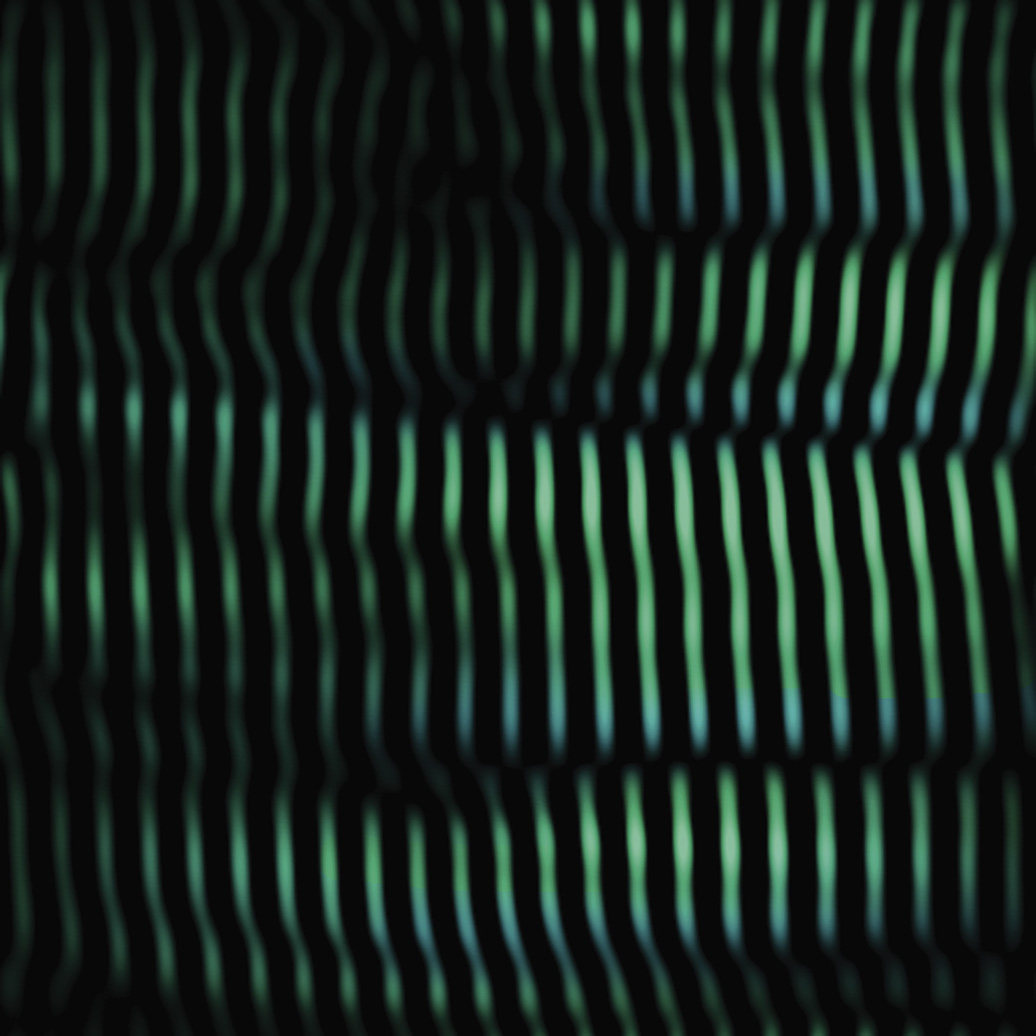
\includegraphics[width=1.0\linewidth]{chap4/4_0}
	% 加星号(*)表示不加编号
	\caption*{ \label{fig:4_0}}
\end{figure}


伦敦皇家学会拥有350年的历史,拥有近200年的传统,每年都会邀请科学家进行公开演讲,并经常进行一些简单的实验。
1952年,其中一项实验成为了热议话题。


两辆固定自行车朝向相反,并通过一条链条连接在一起,当一辆自行车向前踩踏板时,另一辆自行车的踏板就会向后移动(图~\ref{fig:4_1})。


\begin{figure}[!htb]
	\centering
	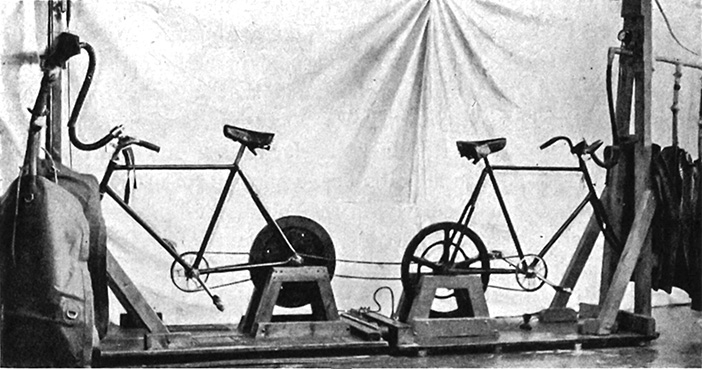
\includegraphics[width=1.0\linewidth]{chap4/4_1}
	\caption{Abbott 等人 (1952) 描述的推拉装置。 \label{fig:4_1}}
\end{figure}


一辆自行车上坐着一位娇小的女子,名叫布伦达$\cdot$比格兰,是肌肉疲劳研究领域的权威专家。
另一辆自行车上坐着一位魁梧的年轻人,名叫默多克$\cdot$里奇,他嫁给了他的自行车“对手”。
演讲者是A$\cdot$V$\cdot$希尔,他因在肌肉产热方面的研究而获得了诺贝尔奖。


里奇听从指令,用尽全力向前蹬,而比格兰则用力蹬着脚蹬,阻止他继续蹬。
想象一下,当观众看到这位娇小的女子轻而易举地阻止了这位身材高大的男人蹬得更快时,他们会有多么惊讶。
很快,他便大汗淋漓,气喘吁吁,而比格兰却几乎毫不费力。
甚至连伦敦市长后来也过来试驾。
“这套设备后来被命名为‘推拉你’,以纪念杜立特医生那只永远不知道自己要往哪个方向跑的双头怪兽,”布伦达$\cdot$比格兰-里奇后来写道。


魔术?小把戏?
并非如此,但它确实表明,肌肉消耗能量和产生力量的方式并非显而易见。
肌肉做正功(例如,在向前蹬踏时充当“马达”)时,它们消耗的能量和产生的热量,比做负功(例如,在向前蹬踏时充当“刹车”)时要多。
一般来说,肌肉产生的力量和消耗的能量,很大程度上取决于它是缩短还是伸长。
希尔实验的经验教训至今仍在日常康复和阻力训练中得到应用。
正如我们将看到的,奇迹发生在分子层面。


本章和下一章将深入探究肌肉内部,探索其结构与功能之间的关系。
肌肉是神奇的生物马达,能够在瞬间悄无声息地产生数千牛顿的力量。
这些力量如此巨大,以至于你小腿的肌肉就能举起一辆小型汽车的尾部。
这些巨大的力量是由数万亿个纳米级分子马达共同作用产生的,这些马达将我们摄入食物中的化学能转化为机械能,使我们能够活动。
这一非凡的功能源于骨骼肌特化的细胞机制和高度组织化的层级结构(图~\ref{fig:4_2})。


\begin{figure}[!htb]
	\centering
	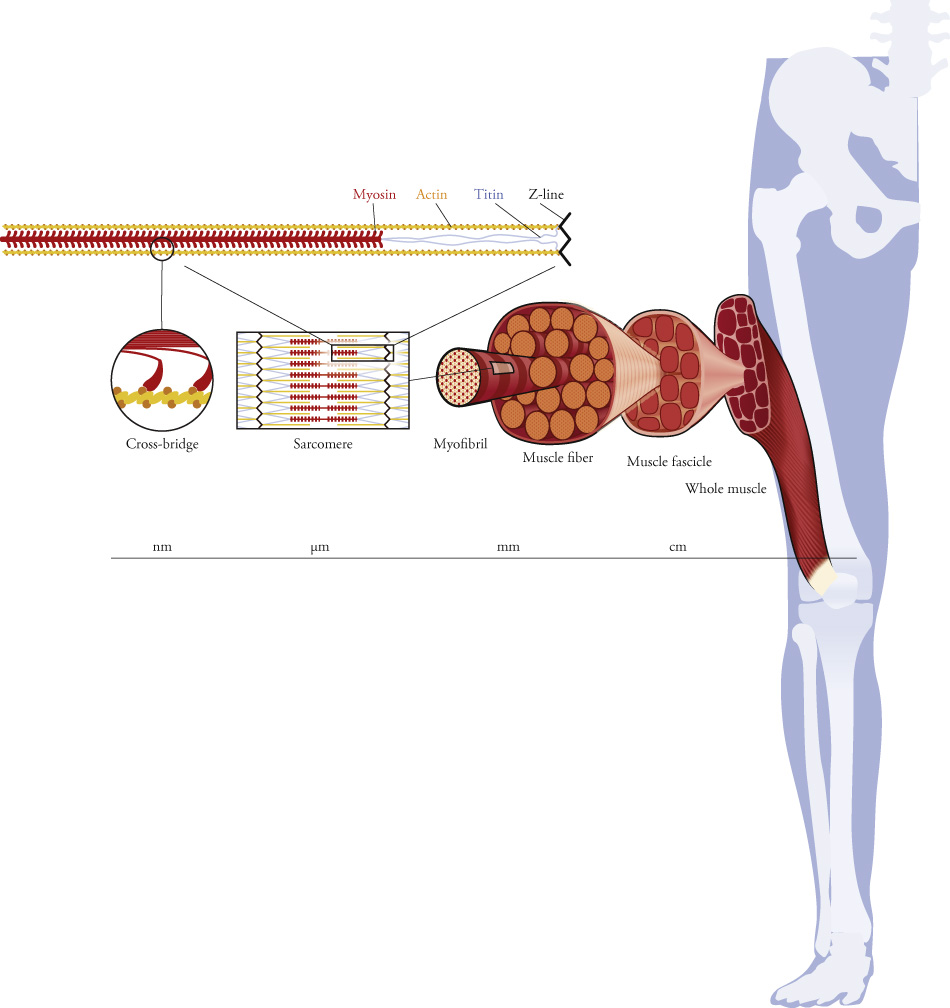
\includegraphics[width=1.0\linewidth]{chap4/4_2}
	\caption{肌肉的多尺度结构。
		骨骼肌具有层次结构,其中有被称为肌球蛋白的纳米级分子马达,每个肌球蛋白仅产生几皮牛顿的力,排列成肌节、肌原纤维、纤维、肌束和整个肌肉,在强力肌肉收缩期间可产生数千牛顿的力。 \label{fig:4_2}}
\end{figure}


接下来两章的组织将大致遵循肌肉的层级结构。
我们将首先在分子层面研究力量的产生过程。
接下来,我们将了解分子马达是如何被包裹在被称为肌节的亚细胞结构中的(活体人体肌节的第一张图像就是在我的手臂上拍摄的,并在本章的开篇图中展示)。
进一步深入,我们将了解单个肌肉细胞如何被神经系统激活,并了解“快肌纤维”和“慢肌纤维”之间的区别。
在第~\ref{chap:chap5}~章中,我们将从宏观层面研究肌肉在体内的排列方式,以及它们如何与肌腱(将肌肉力量传递到骨骼结构)相互作用。


\section{肌肉结构}

从最基本的层面来说,肌肉通过两种细长蛋白质(肌动蛋白和肌球蛋白)的相互作用产生力量。
20 世纪 50 年代初,休$\cdot$赫胥黎通过 X 射线显微镜发现,这些蛋白质平行排列,纤维交织,它们之间的连接被他称为“横桥”。
安德鲁$\cdot$赫胥黎(与休无亲属)同时用不同的方法发现了横桥。
休$\cdot$赫胥黎和安德鲁$\cdot$赫胥黎都怀疑横桥是产生力量的机制,并于 1954 年提出了一个关于这些分子马达如何工作的模型,我们将在下文中解释。
他们的模型一直是解释力量产生的基本范式,尽管随着更多实验数据的收集,该模型变得更加详细。


从尺寸上看,肌纤维排列成束,称为肌束,它们与肌肉纤维一样,长度可达数十厘米。
肌束的横截面积约为 1 毫米。
除了肌纤维外,肌束还包含称为细胞外基质的结缔组织,其中包括胶原蛋白、神经纤维和血管。
在健康的肌肉中,肌纤维紧密排列;
然而,在患病的肌肉中,肌纤维的横截面积可能较小,并被更多的细胞外基质和脂肪隔开。


肌束被更多结缔组织包围,并聚集在一起形成肌肉。
另一层结缔组织鞘被称为筋膜,包裹着肌肉并将其与其他肌肉隔开。
终止于每个肌束末端的肌纤维可以直接附着在骨骼上,但通常它们会连接到肌腱,肌腱随后附着在骨骼上。
肌腱插入肌肉的部分称为腱膜;
肌腱在肌肉外部的部分通常称为游离肌腱。
正如我们将在第~\ref{chap:chap5}~章中看到的,肌腱不仅通过向骨骼传递肌肉力量发挥着重要作用,还在伸展和回缩时储存和释放能量。


\section{横桥循环}

当神经系统激活肌肉时,肌肉会通过数万亿个肌动蛋白和肌球蛋白的协同作用产生力量,这个过程被称为“横桥循环”(图~\ref{fig:4_3})。
这种机制可以粗略地描述为一个分子大小的棘轮。


\begin{figure}[!htb]
	\centering
	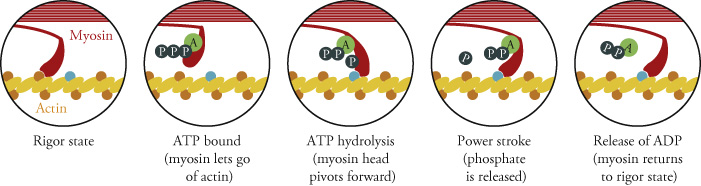
\includegraphics[width=1.0\linewidth]{chap4/4_3}
	\caption{横桥循环描述了肌动蛋白和肌球蛋白相互作用产生力量和运动的过程。
		A 代表腺苷;P 代表磷酸。 \label{fig:4_3}}
\end{figure}

肌球蛋白分子分为 3 个区域,分别称为头部、颈部和尾部。
肌球蛋白头部的独特结构使其能够牢固地结合到肌动蛋白丝上的特定位置(图~\ref{fig:4_3}~第一帧)。
当肌肉需要产生力量时,肌球蛋白头部会接收一种名为三磷酸腺苷 (ATP) 的“燃料”分子。
这刺激肌球蛋白头部从肌动蛋白上分离,向前旋转,并附着到肌动蛋白上的下一个结合位点(图~\ref{fig:4_3}~第二帧和第三帧)。
接下来,肌球蛋白头部围绕颈部区域旋转,这一运动被称为动力冲程 (power stroke),产生几皮牛顿的力,并使肌动蛋白丝彼此滑动约 10 纳米。


当然,不消耗能量就不可能完成机械功。
能量来自于一个化学反应,该反应将一个磷酸离子从三磷酸腺苷中分离出来(图~\ref{fig:4_3}~中的图4),留下二磷酸腺苷(ADP)。
最终,二磷酸腺苷被释放,肌球蛋白恢复到其原始状态,但现在已从其原始位置移位。
当肌球蛋白以这种方式循环时,细丝被拉向肌节中部,从而在化学能转化为机械能的过程中产生张力。


虽然这种机制听起来可能很复杂,但它却是一个优雅而经济的解决方案,解决了如何在分子层面上以可预测的方向产生力的问题。
就像汽车发动机一样,我们的肌肉将化学能转化为机械能,但噪音更小,产生的有毒废气也更少。



\section{肌节结构}

再往上一层,我们来看看肌节。
肌节大致呈圆柱形,长度根据肌肉长度在 1 微米到 5 微米之间变化。
肌节由许多相互交织的“粗”肌丝和“细”肌丝组成,随着肌节长度的变化,这些肌丝会相互滑动。


数百条肌球蛋白尾部捆绑在一起,形成每根粗肌丝,形成棒状结构,肌球蛋白头部以规则的间隔向外放射状延伸(图~\ref{fig:4_4})。
与粗肌丝平行的是细肌丝,它们由 3 种蛋白质组成:
肌动蛋白、原肌球蛋白和肌钙蛋白。
我们已经描述了肌动蛋白,它为肌球蛋白头部提供结合位点。
这些结合位点沿着细肌丝以规则的间隔分布。
原肌球蛋白和肌钙蛋白仅在肌肉被神经系统激活且存在钙离子时才会暴露这些结合位点,从而帮助调节力量的产生。
另一种值得关注的蛋白质(肌联蛋白),将每根粗肌丝附着在肌节的末端(我们称之为 Z 线或 Z 盘)。
正如我们稍后将看到的,肌联蛋白在被动力的产生中起着重要作用,这是一个独立于横桥循环的过程,也是赫胥黎最初的模型所忽略的现象。

\begin{figure}[!htb]
	\centering
	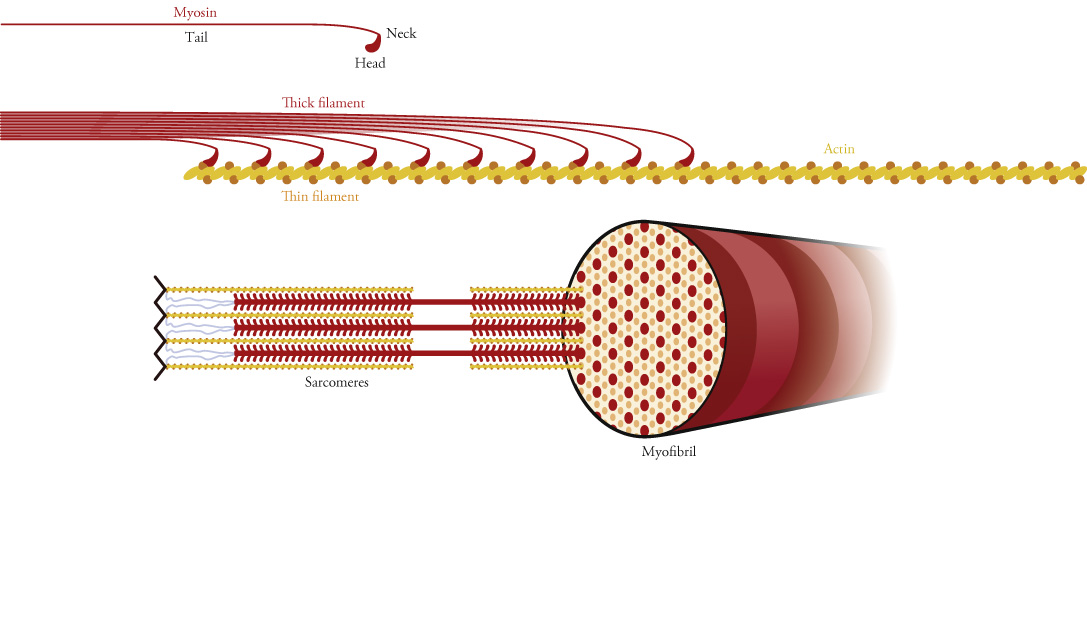
\includegraphics[width=1.0\linewidth]{chap4/4_4}
	\caption{肌球蛋白示意图(顶部)、粗丝和细丝的相互作用示意图(中间)以及肌原纤维横截面,显示粗丝和细丝以高度有序的三维模式排列(底部)。 \label{fig:4_4}}
\end{figure}

肌节在骨骼肌内以规则的模式串联和平行排列,在显微镜下观察骨骼肌组织时,会形成条纹,即明暗交替的带状结构。
您可以在图~\ref{fig:4_5}~中看到这些带状结构,它们分别被称为 I 带、A 带、Z 盘和 M 盘。
严格来说,Z 盘和 M 盘确实是圆盘,但它们通常被称为 Z 线和 M 线,因为它们在二维空间中看起来是这样的。
A 带仅出现在含有肌球蛋白的区域,而 I 带则出现在其他区域。细肌动蛋白丝的一端锚定在 Z 盘上。
粗肌球蛋白丝的一端附着在 M 盘的结构上,另一端通过肌联蛋白分子固定在 Z 盘上。
骨骼肌有时被称为“横纹肌”,与“平滑肌”相对,例如控制血管口径的肌肉,它们没有组织成肌节,也没有呈现条纹图案。

\begin{figure}[!htb]
	\centering
	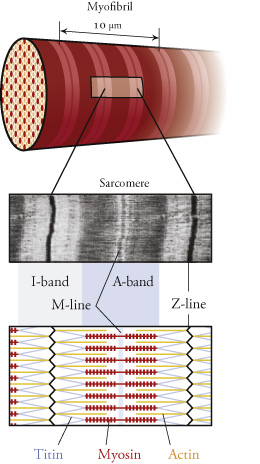
\includegraphics[width=0.5\linewidth]{chap4/4_5}
	\caption{肌原纤维示意图(上)展示了其高度组织化的微观结构。
		肌肉显微镜图像(中)和肌节示意图(下)分别标记了I带、A带、M线和Z线。
		肌节的末端由Z线定义。 \label{fig:4_5}}
\end{figure}


\section{力-长度关系}

肌节所能产生的最大力量会随着其长度的变化而变化。
长度和张力之间的关系可以用滑动丝理论来解释,该理论由两个研究小组于 1954 年独立提出。
Andrew Huxley 和 Rolf Niedergerke(在单根肌纤维中)以及 Hugh Huxley 和 Jean Hanson(在分离的肌原纤维中)证明,在主动肌肉收缩过程中,肌小节带不会变窄,这推翻了粗肌丝缩短的流行理论。
他们给出的解释是,随着肌节长度的变化,粗肌丝和细肌丝会相互滑动。
因此,肌节的长度会影响肌动蛋白和肌球蛋白之间“重叠”的量,或者说靠近细肌丝上结合位点的肌球蛋白头部的数量。
随着肌球蛋白头部和肌动蛋白结合位点之间横桥数量的增加,激活的肌节内的张力也会增加。


如图~\ref{fig:4_6}~所示,激活的肌肉中横桥循环所能产生的力随肌节长度而变化。
该主动力-长度曲线通常被描述为具有三个区域:
上升区,其中力随肌节长度的增加而增加;
平台区,其中力保持在最大值;
下降区,其中力随肌节长度的增加而减小。
平台区涵盖一系列肌节长度,称为“最佳”范围,其中肌球蛋白头部和肌动蛋白结合位点之间的相互作用数量达到最大值。
最佳肌节长度因脊椎动物而异,但通常在 2.2 至 2.7 μm 之间,在人类骨骼肌中约为 2.7 μm。
当肌节长度超过最佳范围时,肌动蛋白和肌球蛋白的重叠量会减少,横桥循环所能产生的力量也会减少。
当肌节长度略短于最佳长度时,源自肌节两端的细肌丝开始在肌节中部重叠并相互干扰,导致所谓的“浅上升区”的力量减弱。
当肌节长度更短时(在“陡峭上升区”),粗肌丝会与Z盘碰撞并变形,产生阻碍横桥循环作用的力量。
由于肌肉由串联和并联排列的肌节组成,我们可以观察到肌肉主动收缩过程中力量与长度之间的类似关系。

\begin{figure}[!htb]
	\centering
	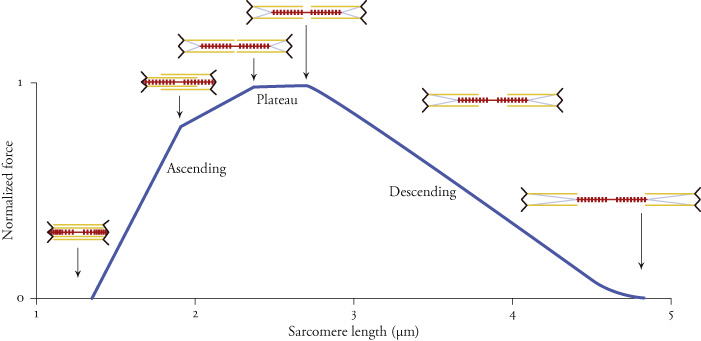
\includegraphics[width=0.5\linewidth]{chap4/4_6}
	\caption{肌节产生的主动力与其长度有关。粗肌丝和细肌丝相互滑过时,力会发生变化。
		在肌节的上升支,力随长度增加而增大,达到平台期;
		在肌节的下降支,力随长度增加而减小。
		当横桥数量达到最大时,力的产生达到峰值\cite{gordon1966variation}。 \label{fig:4_6}}
\end{figure}





\chapter{肌肉结构和肌肉动力学} \label{chap:chap5}


如果你想理解功能,那就研究结构。

\begin{flushright}
	——弗朗西斯$\cdot$克里克
\end{flushright}


\begin{figure}[!htb]
	\centering
	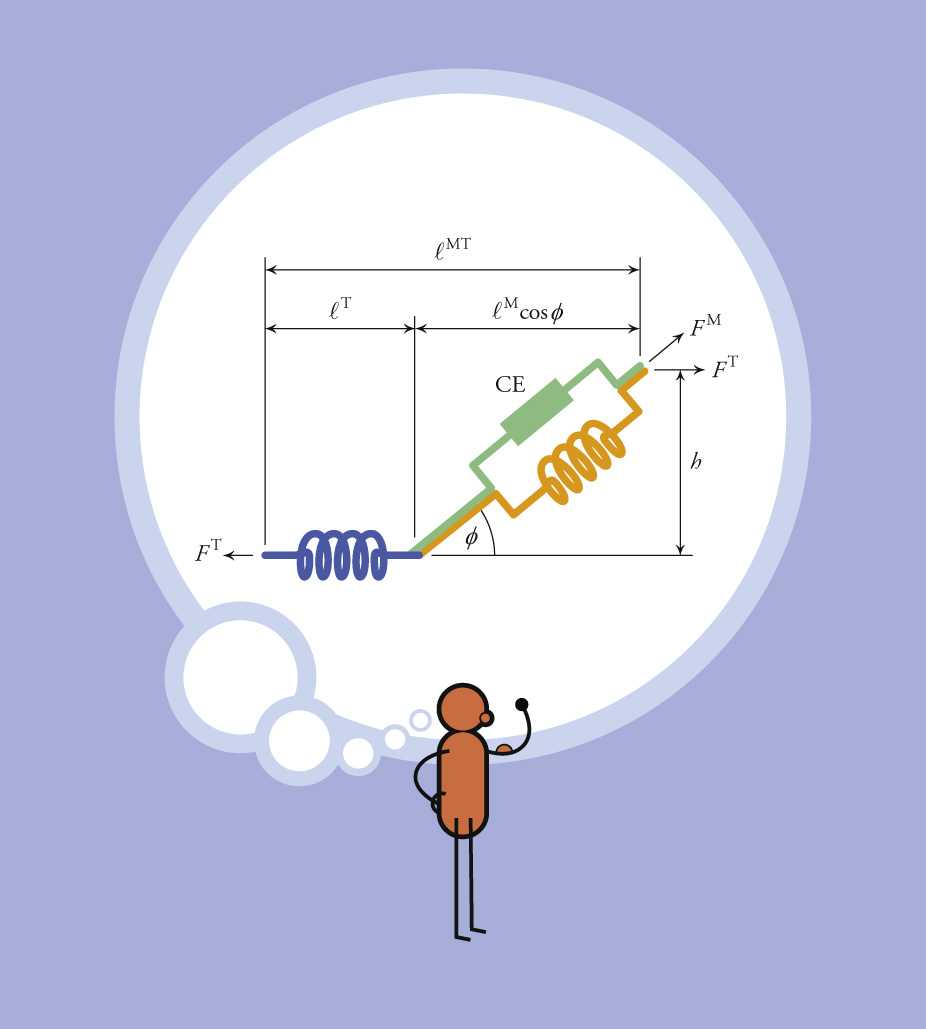
\includegraphics[width=1.0\linewidth]{chap5/5_0}
	% 加星号(*)表示不加编号
	\caption*{ \label{fig:5_0}}
\end{figure}


为了理解人类和动物的运动,研究人员开展了各种各样的实验。
生物力学家通过测量数千人的关节运动、地面反作用力和肌电信号来研究全身运动。
生理学家研究了单个肌肉,以表征肌肉激活和力量产生的动态。
肌肉驱动模拟使我们能够将这 2 个领域联系起来,将全身运动的生物力学测量与针对单个肌肉进行的实验相结合。
我们将在第~\ref{chap:chap10}~至~\ref{chap:chap12}~章中看到,肌肉驱动模拟可以深入了解肌肉在产生运动中的作用,并提供一些在人体运动时几乎无法测量的重要量估计值,例如肌肉产生的力量和它消耗的能量。


肌肉动力学建模对于创建肌肉驱动的运动模拟至关重要。
然而,一刀切的模型并不适用,因为每块肌肉都有其独特的结构来适应其独特的功能。
例如,一些肌肉负责手指的精细运动控制,而另一些肌肉则在运动过程中支撑身体重量(图~\ref{fig:5_1})。
所有骨骼肌都具有肌节的层级排列,但肌肉在几个重要方面存在差异。
这些差异包括它们的大小和结构,以及肌肉纤维的几何排列。
因此,肌肉的计算模型必须捕捉所有肌肉共同的肌肉力量产生特征,同时还要能够表征每块肌肉的独特特征。


\begin{figure}[!htb]
	\centering
	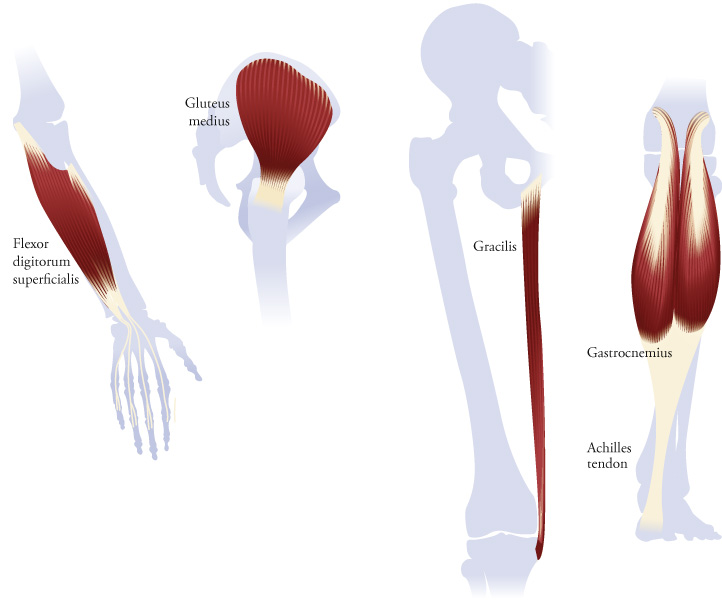
\includegraphics[width=1.0\linewidth]{chap5/5_1}
	\caption{全身肌肉的结构和功能各不相同。
		浅屈指肌(最左侧)通过 4 条肌腱控制手指屈曲;
		宽阔的臀中肌和纤细的股薄肌产生髋关节外展和内收力矩;
		腓肠肌(最右侧)通过较长的跟腱止于跟骨。 \label{fig:5_1}}
\end{figure}


在本章中,我们将了解如何创建一个通用的肌肉力量产生模型,以及如何对其进行定制以代表身体中的几乎任何肌肉。
我们将要描述的肌肉模型属于以 A. V. Hill 命名的一类模型,除了我们在第~\ref{chap:chap4}~章中看到的“推我拉你”实验之外,他还进行了许多肌肉的基础研究。
我的博士生导师 Felix Zajac 改进了 Hill 型模型,并将其带入了现代计算机模拟时代\cite{zajac1989muscle}。
具体来说,Zajac 开发了一个仅包含 4 条通用曲线和 5 个肌肉特定参数的模型,所有这些参数都可以从实验数据中得出并用于调整模型。
Zajac 模型的简单性对于涉及数十块肌肉的动态模拟至关重要,但它足够详细,可以表示不同大小、强度和结构的肌肉的动态。


图~\ref{fig:4_18}~总结了所有肌肉共同的肌肉力量产生特征。
这些特征包括 3 条曲线,描述肌肉长度与其产生的力之间的非线性关系:主动力-长度曲线、被动力-长度曲线和力-速度曲线。
由于肌肉通过肌腱附着在骨骼上,我们还必须考虑这种结缔组织的特性,我们用肌腱的力-长度曲线来描述它。
我们使用 5 个参数缩放这些通用曲线以表示特定的肌肉:
(1)最佳肌纤维长度 $l_o^M$;
(2)最佳纤维长度下的肌纤维羽状角 $\phi_o$ ;
(3)最大等长肌肉力量,$F_o^M$;
(4)最大肌肉收缩速度 $v_\text{max}^M$;
和(5)肌腱松弛长度,$l_s^T$。
本章首先介绍这 5 个特定于肌肉的参数。
我们将了解每个参数如何影响肌肉力量,并将其纳入肌肉-肌腱动力学模型中。


\section{最佳肌纤维长度$l_o^M$}

正如我们在第~\ref{chap:chap4}~章中看到的,肌节能够产生的主动力取决于其长度(图~\ref{fig:4_6})。
肌节能够产生最大等长收缩力的长度称为其最佳长度。
由于肌纤维由多个($n$)个首尾相连的肌节组成,因此肌纤维也存在一个最佳长度($l_o^M$),当其每个组成肌节都达到其最佳长度($l_o^S$)时,肌纤维便会达到该最佳长度:
%
\begin{equation}
	l_o^M = n l_o^S \label{eq:5_1}
\end{equation}

公式~\ref{eq:5_1}~假设肌纤维上串联的所有肌节长度相同。
肌肉在运动过程中会伸长和缩短,这会影响肌节粗肌丝和细肌丝相互滑动时产生的主动力。
最佳长度较长的肌纤维(即串联肌节较多)具有更宽的主动力-长度曲线,并且可以在更宽的长度范围内产生其最大主动力的很大一部分(图~\ref{fig:5_2}~顶部)。
增加肌纤维的最佳长度也会增加其最大缩短速度($v_{\text{max}}^{\text{M}}$):

\begin{figure}[!htb]
	\centering
	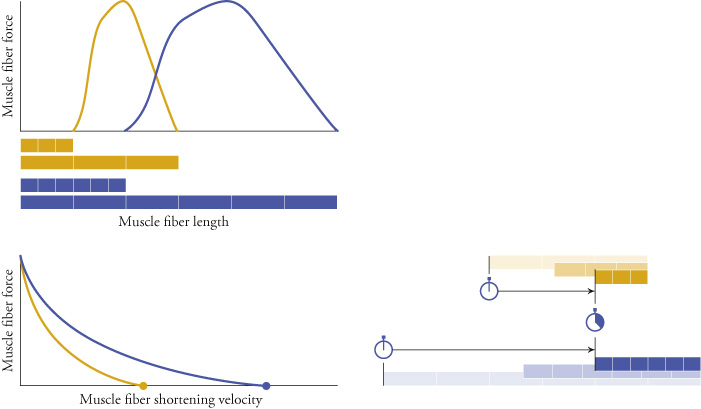
\includegraphics[width=1.0\linewidth]{chap5/5_2}
	\caption{最佳肌纤维长度较长的肌肉,其主动力-长度曲线(上图)更宽,最大缩短速度也更高(下图)。
		请注意,长肌纤维(蓝色)的示意图中,肌节数量是短肌纤维(橙色)的 2 倍,因此长肌纤维在给定时间内可以缩短 2 倍的距离(右下图)。 \label{fig:5_2}}
\end{figure}

\begin{equation}
	v_{\text{max}}^M = n v_{\text{max}}^S \label{eq:5_2}
\end{equation}
%
其中,$v_\text{max}^S$表示肌节的最大缩短速度。
因此,随着肌肉最佳纤维长度的增加,力-速度曲线也会变宽(图~\ref{fig:5_2}底部)。


生物肌肉由长度不同的肌束构成,肌束本身包含长度也不同的纤维,这些纤维甚至可能终止于肌束内。
然而,在我们的模型中,我们假设肌肉中的所有纤维长度相同(许多肌肉,但并非所有肌肉),肌腱动力学模型都做出了这一假设。
我们进一步假设所有纤维都是直的、平行的且共面的。
因此,为了表征肌肉的力-长度和力-速度特性,我们只是放大了肌纤维的相应特性,而这些特性仅仅是肌节相同特性的放大版本。



\section{最佳纤维长度下的肌纤维羽状角$\phi_o$}

肌肉通常通过肌腱附着于骨骼。
在平行纤维肌腱中(例如缝匠肌),其纤维沿着肌腱方向排列(图~\ref{fig:5_3})。
在大多数其他肌肉中,例如股直肌,其纤维与肌腱呈锐角排列;我们称这些肌肉为羽状肌。
“羽状肌”一词源于拉丁语,意为“羽毛状”,而羽状肌的结构确实让人联想到鸟类的羽毛。

\begin{figure}[!htb]
	\centering
	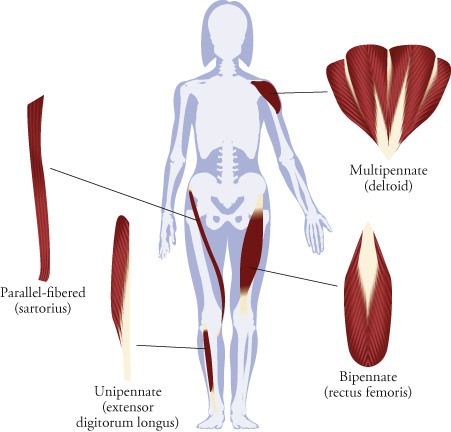
\includegraphics[width=0.8\linewidth]{chap5/5_3}
	\caption{具有不同结构肌肉的例子:
		平行纤维肌肉、单羽状肌肉、双羽状肌肉和多羽状肌肉。 \label{fig:5_3}}
\end{figure}

如果所有肌纤维都附着在肌腱的一侧,我们称该肌肉为单羽状肌;
如果肌纤维附着在肌腱的两侧,则称该肌肉为双羽状肌。
在多羽状肌中,肌腱分支和肌纤维结构可能很复杂。
因此,我们假设给定肌肉中的所有纤维都以相同的角度(称为羽状角 ($\phi$))附着于肌腱,并采用图~\ref{fig:5_4}~所示的肌肉-肌腱几何模型。
由此,我们得到肌纤维中的力 ($F^M$) 和肌腱中的力 ($F^T$) 之间的以下关系:

\begin{figure}[!htb]
	\centering
	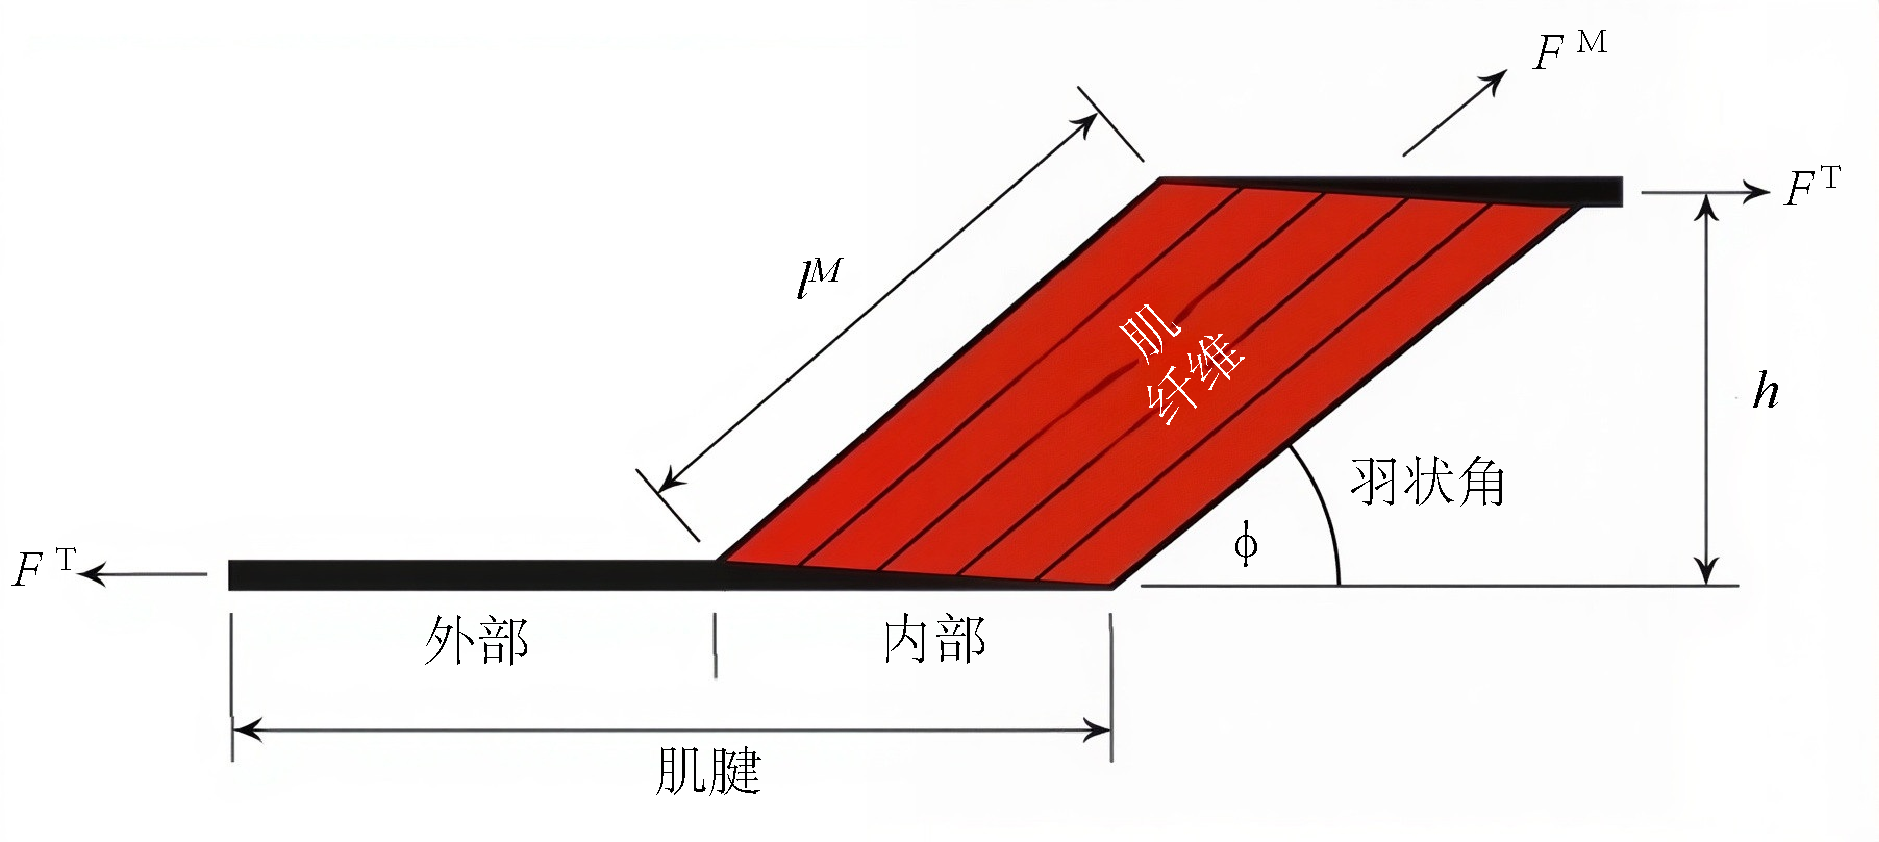
\includegraphics[width=0.75\linewidth]{chap5/5_4}
	\caption{\textit{肌纤维}和\textit{肌腱}的简化几何表示。
		\textit{肌纤维}被假设为直的、平行的、共面的、等长的,并以相同的\textit{羽状角} ($\phi$) 附着于\textit{肌腱}。
			当\textit{肌纤维}缩短或伸长,\textit{羽状角}增大或减小时,平行四边形的高度 $h$(以及面积)保持不变\cite{zajac1989muscle}。 \label{fig:5_4}}
\end{figure}

\begin{equation}
	F^T = F^M cos(\phi) 
	\label{eq:5_3}
\end{equation}

现在,参考图~\ref{fig:5_4},我们可以解释生物肌肉如何在纤维长度发生变化的情况下保持体积恒定。
随着图中纤维的缩短,想象一下它们以这样的方式缩短,使得图~\ref{fig:5_4}~中的平行四边形保持相同的高度 $h$。
平行四边形的顶部将保持不变,但底部将被向右拉,平行四边形将变得更接近矩形。
然而,只要高度保持不变,面积也将保持不变,这符合平行四边形面积等于其底边和高乘积的几何规则。
我们以二维方式绘制了该图,但三维运动类似,并确保肌肉的体积不变。
简而言之,羽状肌不是通过膨胀来维持体积,而是通过剪切来维持体积。


在上述过程中,羽状角不断增大,从纤维传递到肌腱的力不断减小,直到纤维与肌腱垂直,图中的肌肉呈矩形(即$\phi$ = 90度)。
我们使用参数$\phi_o$表示肌纤维达到最佳长度时的羽状角(即$l^M = l_o^M$)。
我们所描述的固定高度近似法可能会对收缩时明显隆起的肌肉引入误差,但它为研究肌肉结构的功能含义提供了一个简单的几何模型。


除了公式~\ref{eq:5_3}~中表达的关系外,羽状肌在决定肌肉的产力能力方面也起着至关重要的作用。
一般来说,羽状肌角度越大,在给定体积内能够容纳的肌肉纤维越多。
想象一下在矩形房间铺设硬木地板的类似情况:
可以使用相对较少的长木板来延伸房间的长度,或者使用大量较短的木板以对角线方向铺设。
同样,与相同体积的平行纤维肌肉相比,羽状肌的纤维更短,因此主动力-长度曲线和力-速度曲线更窄(图~\ref{fig:5_2})。
当然,羽状肌也包含更多的纤维,其后果将在下一节探讨。



\section{最大等长肌肉力 $F_o^M$}

我们 5 个肌肉参数系列中的第三个参数相对容易理解,但测量起来却不那么容易。
这就是最大等长肌肉力。
它被定义为肌肉在最大程度激活并保持最佳纤维长度时产生的力。


对于活体人体来说,最大等长肌力很难测量,因为我们无法将一块肌肉与其他肌肉分离,并只对该肌肉施加阻力。
因此,我们使用一个称为\textit{生理横截面积}(图~\ref{fig:5_5})的指标。
这是肌肉垂直于纤维方向的横截面积。
需要注意的是,在羽状肌中,该横截面积与肌肉的纵轴倾斜。
最大等长肌力可以通过以下方式估算:

\begin{figure}[!htb]
	\centering
	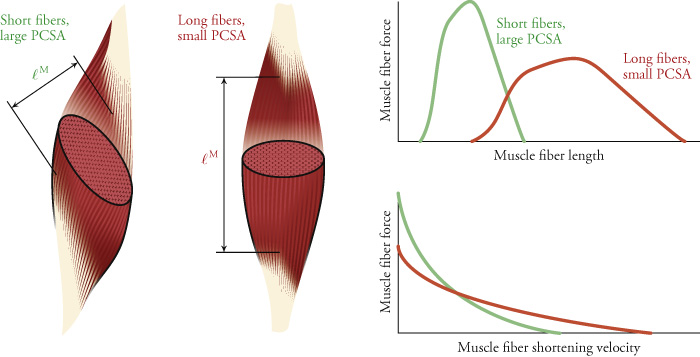
\includegraphics[width=1.0\linewidth]{chap5/5_5}
	\caption{左图所示的肌肉体积相同,但\textit{生理横截面积}、最佳纤维长度和羽状角不同。
		羽状肌越多,产生的主动力越大,但纤维越短;
		因此,其主动力-长度曲线和动力-速度曲线更高,但更窄\cite{lieber2002skeletal}。 \label{fig:5_5}}
\end{figure}

\begin{equation}
	F_o^M = \text{PCSA} \sigma_o^M
	\label{eq:5_4}
\end{equation}
%
其中 $\sigma_o^M$ 是肌肉的比张力(也称为峰值等长应力),即单位面积可产生的最大肌肉力。
在构建健康肌肉模型时,该参数的典型值为 $\sigma_o^M = 0.3 \; \text{MPa}$ 。


在上一节中,我们注意到,羽状肌的纤维比相同体积的平行纤维肌更短,但数量也更多。
因此,尽管羽状肌的力-长度和力-速度曲线较窄,但这些曲线也会更高,因为羽状肌的\textit{生理横截面积}(以及因此产生的最大等长力)更大(图~\ref{fig:5_5})。


肌肉纤维的长度和收缩速度不仅仅受其几何形状的影响,我们将在接下来的两节中看到这一点。
尽管如此,我们已经可以观察到肌肉的结构如何影响其所能执行的功能范围:
在其他条件相同的情况下,羽状肌能够比相同体积的平行纤维肌产生更大的力量,但其长度范围较小,收缩速度也较低。



\section{最大肌肉收缩速度$v_\text{max}^M$}

到目前为止,我们已经介绍了 3 个与肌肉纤维几何排列相关的变量。
为了确定肌肉的最大收缩速度,我们现在引入一个概念:
肌肉纤维有 2 种类型:快肌纤维和慢肌纤维。
在单次收缩实验中(图~\ref{fig:4_12}),快肌纤维具有更快的上升时间和松弛时间,并且最大收缩速度也更高——大约为每秒 10 个最佳纤维长度 (10 $l_o^M / s$),而慢肌纤维约为 3 $l_o^M / s$ 个。
哺乳动物的肌肉同时包含这 2 种类型的纤维,但快肌纤维与慢肌纤维的比例会因肌肉的功能而异。
例如,腓肠肌含有大量的快肌纤维,这些纤维在需要快速产生巨大力量的活动(例如短跑)中被募集。
邻近的比目鱼肌主要由慢肌纤维组成,这些慢肌纤维非常适合在长时间站立时产生力量,因为慢肌纤维耐疲劳。


肌纤维不仅以其收缩速度区分,还以其产生ATP的方式区分。
有氧(即利用氧气)产生ATP的肌纤维比无氧(即无氧)产生ATP的肌纤维更耐疲劳。
慢肌纤维往往耐疲劳,而快肌纤维则易疲劳。
人类和其他一些动物拥有第三种肌纤维类型,因此我们通常将肌纤维分为I型(慢速,耐疲劳)、IIA型(快速,中度易疲劳)或IIB型(极快,高度易疲劳)。
通过强化训练可以增加快速且仅中度易疲劳的肌纤维比例。


回想一下第~\ref{chap:chap4}~章,运动单位大小各异,中枢神经系统会按照亨尼曼大小原则(图~\ref{fig:4_13})从小到大依次募集运动单位。
除了大小不同之外,运动单位所含纤维的类型也有所不同,同一运动单位中的所有纤维都属于同一类型。
最小的运动单位通常由 I 型纤维组成,最先被募集,其次是由 IIA 型纤维组成的稍大的运动单位。
最大的运动单位包含 IIB 型纤维,通常最后被募集。
因此,在低激活度下(例如在安静站立时可能观察到),主要募集的是慢肌、抗疲劳的运动单位。
因此,在低激活度下,肌肉的最大收缩速度可能会降低;
然而,在肌肉-肌腱动力学模型中,通常假设其为常数 10 $l_o^M/s$。


粗略地说,家禽和鱼类的可疲劳肌纤维和抗疲劳肌纤维是分开的(图~\ref{fig:5_6})。
相反,哺乳动物的肌肉中可疲劳肌纤维和抗疲劳肌纤维是交替分布的。
这就是为什么鸡肉菜肴可以用白肉或黑肉来制作,而牛肉菜肴却不能。
颜色差异的原因是深色肌肉(或肉)富含一种叫做肌红蛋白的蛋白质,这种蛋白质在肌肉中储存氧气,使肌肉颜色变深,使其更耐疲劳。
鸡腿的深色肉由用于长时间站立和奔跑的腿部肌肉(抗疲劳、慢肌纤维)组成。
白色的胸肉由仅用于短时间飞行的肌肉(可疲劳、快肌纤维)组成。
在人类中,单个肌纤维要么是“深色”的,要么是“白色”,但这两种纤维类型都散布在每块肌肉中。


\begin{figure}[!htb]
	\centering
	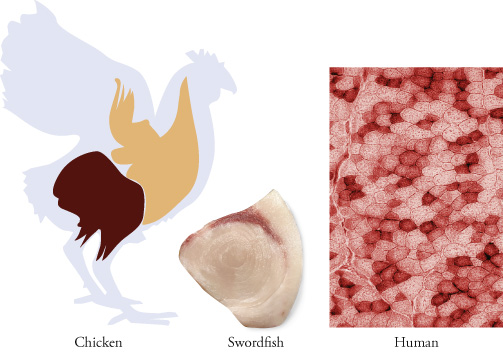
\includegraphics[width=0.8\linewidth]{chap5/5_6}
	\caption{鸡和鱼类的某些肌肉主要由抗疲劳的慢肌纤维(深色肉)组成,而另一些肌肉则由易疲劳的快肌纤维(白肉)组成。
		在人类和其他哺乳动物中,各种类型的纤维散布在每块肌肉中。
		人体纤维染色图像显示了不同的纤维类型,由 Richard Lieber 提供。 \label{fig:5_6}}
\end{figure}


\section{肌腱松弛长度 $l_s^T$}

到目前为止,我们讨论的所有参数都与肌腱无关。
在我们的希尔模型中,我们将肌腱描述为非线性弹簧。
本节介绍 5 个参数中的第五个参数,称为肌腱松弛长度,以及 4 个通用无量纲曲线中的第四个参数,称为肌腱力-长度曲线。
我们根据应力和应变之间的实验测量结果推导出力-长度曲线(图~\ref{fig:5_7})。


\begin{figure}[!htb]
	\centering
	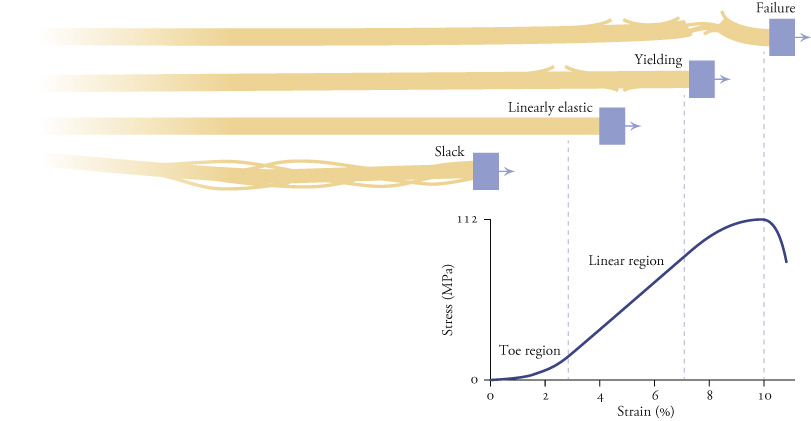
\includegraphics[width=0.8\linewidth]{chap5/5_7}
	\caption{肌腱应力-应变关系。 \label{fig:5_7}}
\end{figure}

在该图中,横轴表示肌腱的\textit{应变},用其长度相对于静止且未受力时的长度的百分比表示。
静止长度即为松弛长度,用 $l_s^T$ 表示。
任意给定时刻肌腱的应变 ($\epsilon^T$) 定义如下:
\begin{equation}
	\epsilon^T = \frac{l^T - l_s^T}{l_s^T} 
	\label{eq:5_5}
\end{equation}
% 
其中 $l^T$ 是肌腱的当前长度,$l_s^T$是其松弛长度。


图~\ref{fig:5_7}~中的纵轴表示肌腱单位横截面积产生的力,称为应力。
在线性弹簧中,应力与应变的关系图是一条直线,其斜率表示弹簧的刚度。
由于肌腱充当非线性弹簧,因此应力-应变曲线不是直线,并且它具有 3 个具有不同刚度特征的区域。
在脚趾区域,当肌腱拉伸约 0\% 到 3\% 时,它会更加柔顺(“有弹性”),随着肌腱的伸长和其组成胶原纤维的展开,其刚度逐渐增加。
在应力-应变曲线的线性区域,当肌腱拉伸约 3\% 到 7\% 时,肌腱具有恒定的刚度;
在此区域,它的行为类似于线性弹簧。
最后,超过 10\% 的应变,肌腱开始出现机械故障,并且存在很高的受伤风险。
我们通常假设内部肌腱(腱膜)和外部肌腱具有相同的材料特性和应变。
有实验证据支持上面给出的应变值,但有人认为肌腱在断裂前可以承受高达 15\% 的更高应变值。


肌腱会影响其所附着肌肉的长度,从而影响其产力能力(图~\ref{fig:5_8})。
如果肌腱的松弛长度相对于肌纤维的长度较短,则肌腱的拉伸几乎不会产生影响:
即使这样的肌腱承受很大的应变,其绝对长度变化(以及肌纤维缩短的量)也只是肌纤维最佳长度的一小部分。
相反,如果肌腱的松弛长度相对于肌纤维的最佳长度较长,则肌肉产力时肌腱会大幅拉伸,导致肌纤维明显缩短,并改变产生的主动力。
图~\ref{fig:5_9}~显示,较长的肌腱还可以增加肌肉-肌腱单元产力的长度范围。
通过这 2 种方式,肌腱都会显著影响肌肉功能。
当然,当肌腱损伤导致肌肉几乎无法使用时,肌腱的作用尤为明显。
正如我们将在第~\ref{chap:chap12}~章中看到的,肌腱在跑步过程中伸展和回缩时也在能量的储存和释放中发挥着重要作用。


\begin{figure}[!htb]
	\centering
	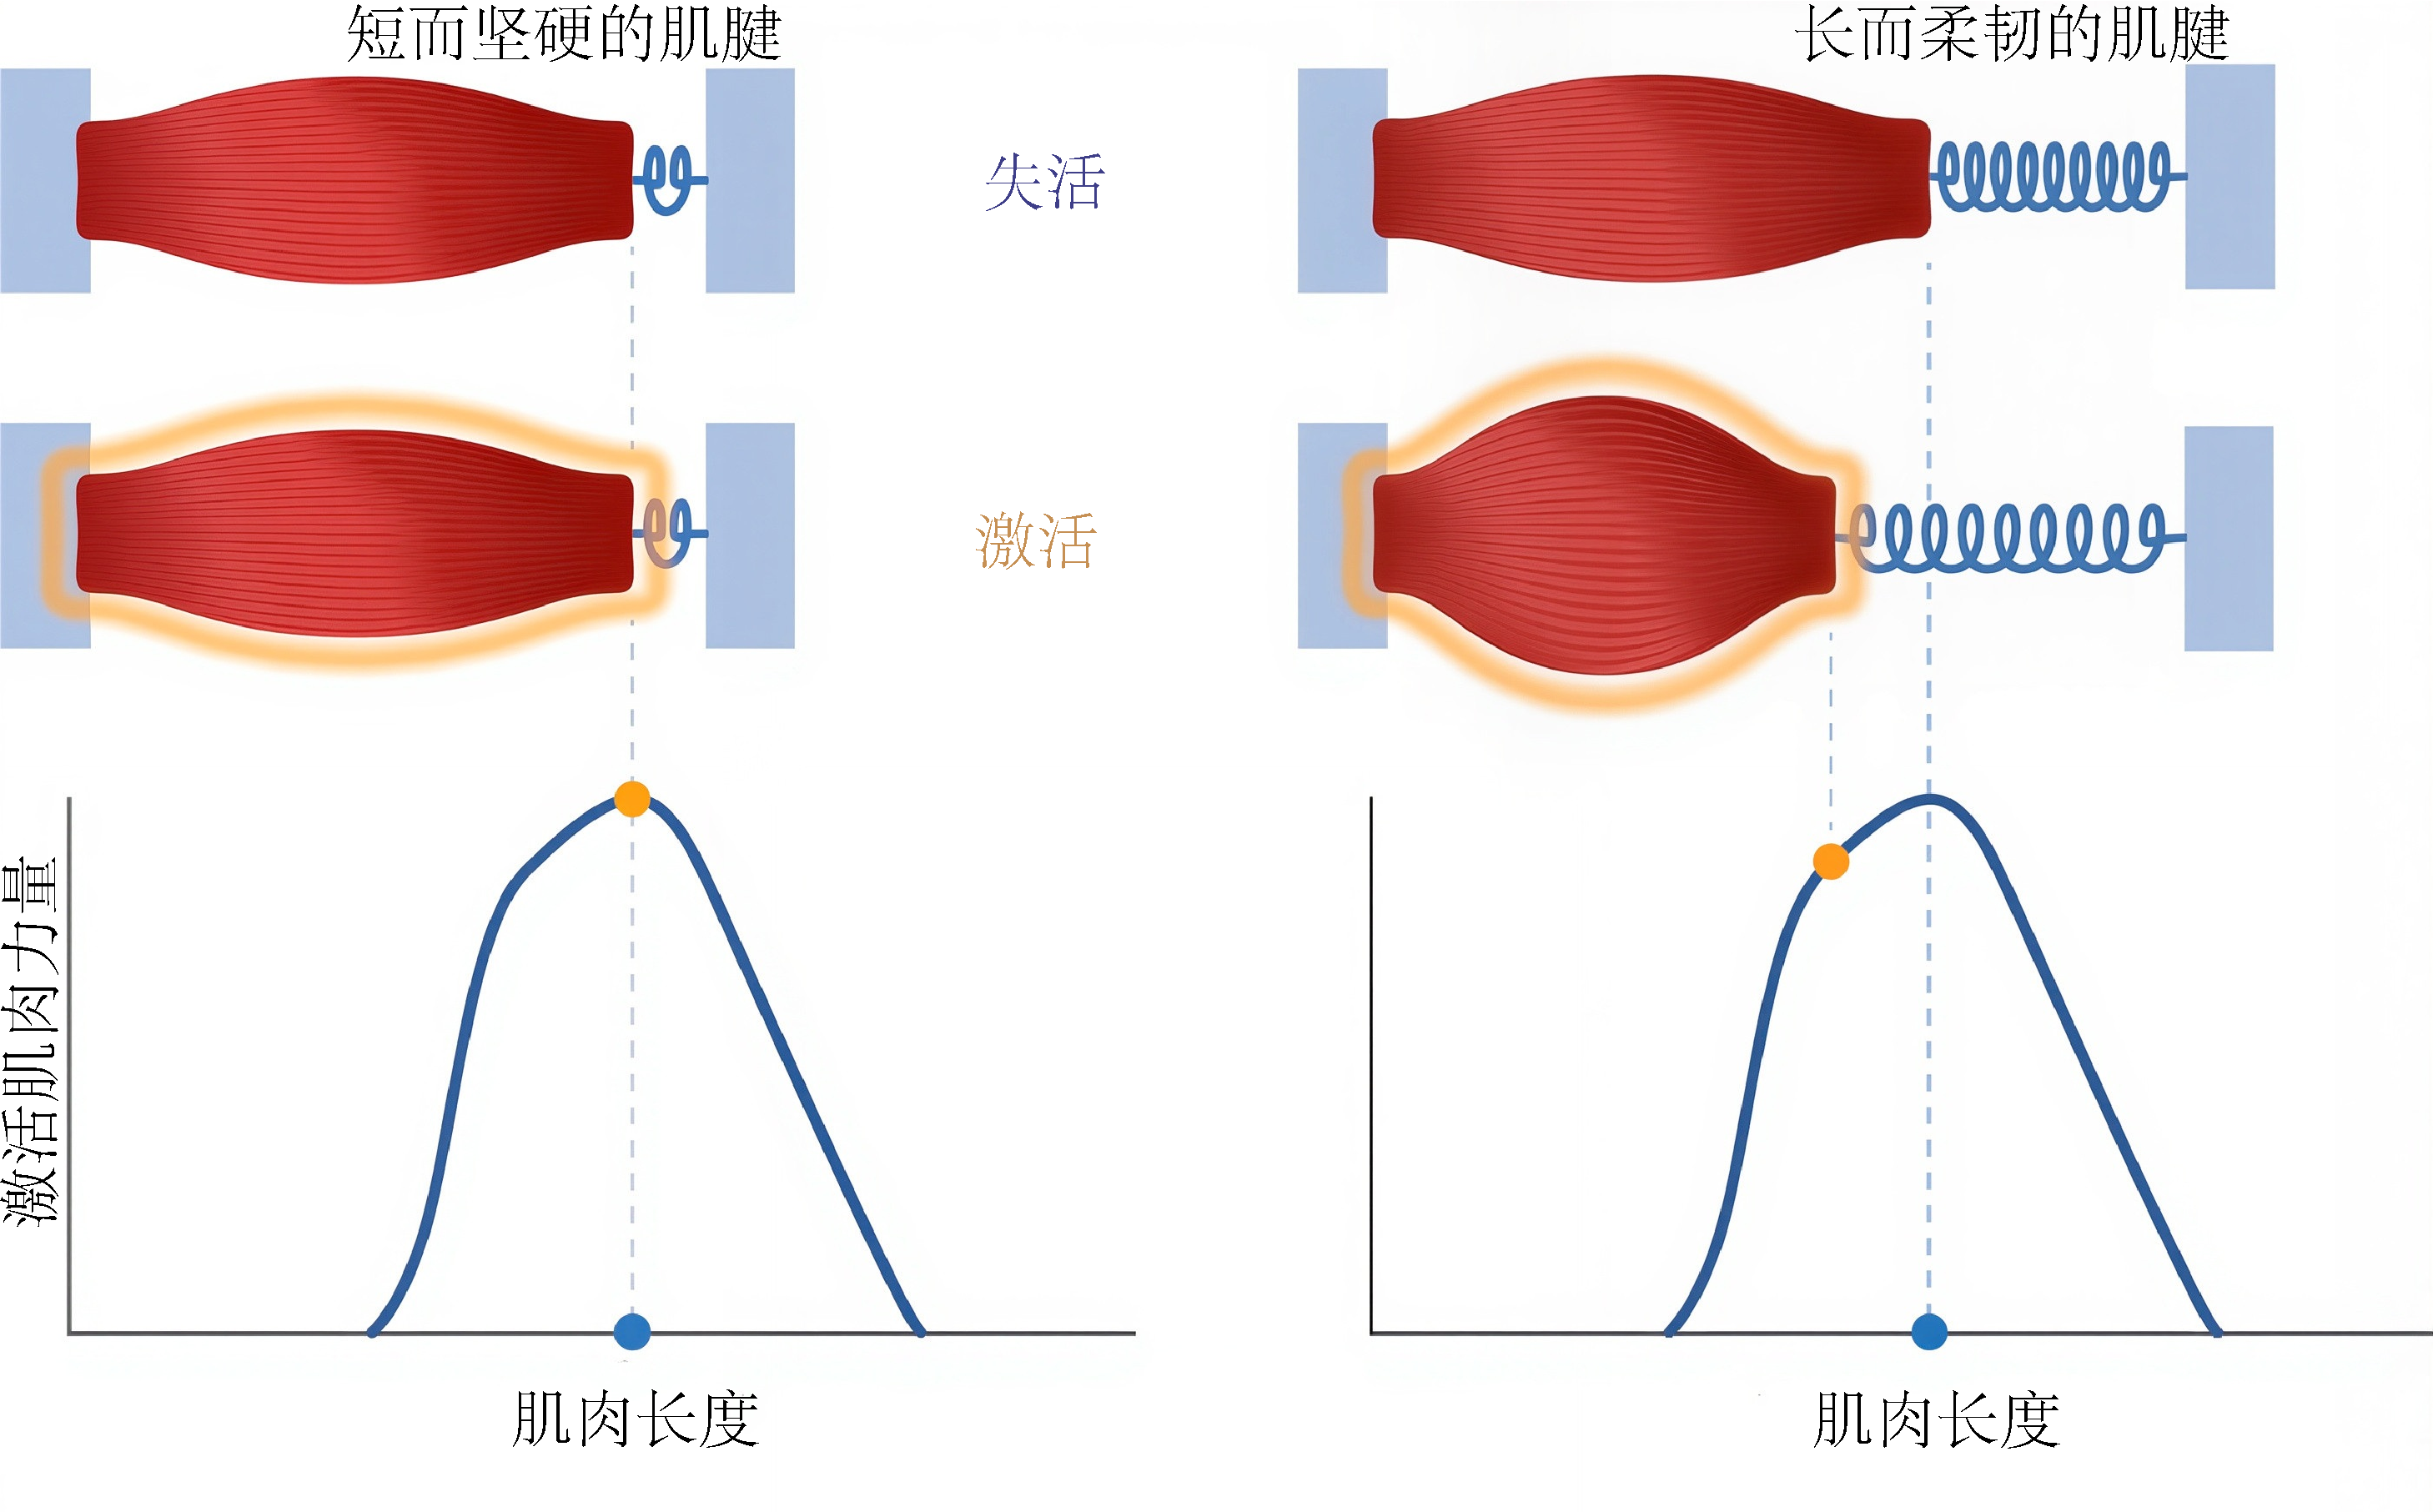
\includegraphics[width=1.0\linewidth]{chap5/5_8}
	\caption{肌腱的柔顺性会影响肌肉力量的产生。
		在图示的两种情况下,平行纤维肌肉在非活动状态时处于最佳长度(上)。
		如果肌腱相对较短且僵硬(左),则肌肉活动时肌纤维的长度变化可以忽略不计。
		如果肌腱较长且柔顺性良好(右),则肌肉活动时肌腱会拉伸,从而缩短肌纤维并减少产生的力量。 \label{fig:5_8}}
\end{figure}


\begin{figure}[!htb]
	\centering
	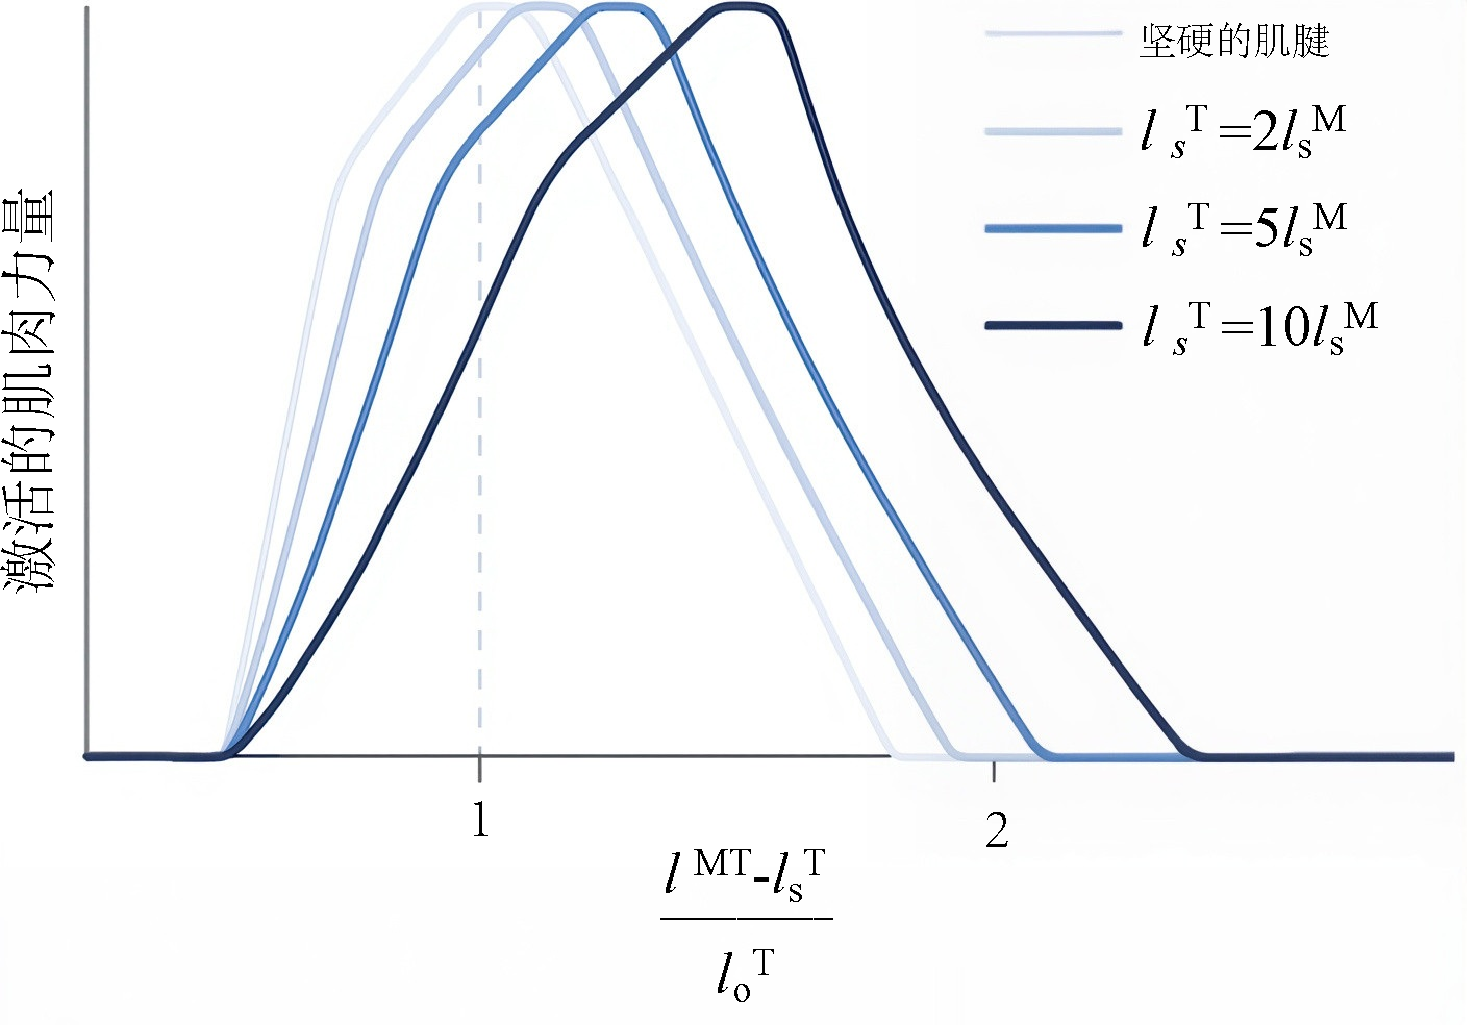
\includegraphics[width=0.6\linewidth]{chap5/5_9}
	\caption{肌腱柔顺性对主动力-长度曲线的影响。
		增加肌腱相对于最佳肌纤维长度的松弛长度(即增加肌腱柔顺性),可以扩大肌肉-肌腱执行器产生主动力的长度范围。 \label{fig:5_9}}
\end{figure}



\section{测量肌肉特定参数}

总而言之,我们定义了 5 个肌肉特异性参数,列于表~\ref{tab:5_1},这些参数捕捉了身体肌肉之间的大部分变异性。
我们在表 5.2 中列出了下肢主要肌肉的这些参数值。
为方便起见,我们通常将力、速度、肌肉长度和肌腱长度分别除以 、 、 和 来进行归一化,并使用波浪号表示归一化后的量(例如 )。


\begin{table}[htbp]
	\caption{Hill 型模型使用的 5 个肌肉特定参数} \label{tab:5_1} \centering
	\begin{tabular}{ccc} % l水平左居中,c水平居中
		\toprule
		肌肉特异性参数 & 符号 & 典型单位  \\
		\midrule
		最佳纤维长度下的羽状角 & $\phi_o$ &  度 \\
		\midrule
		最大等长力量 & $F_o^M$ &  牛顿 \\
		\midrule
		最大收缩速度 & $v_\text{max}^M$ &  $l_o^M / s$ \\
		\midrule
		肌腱松弛长度 & $l_s^T$ &  厘米 \\
		\bottomrule
	\end{tabular}
\end{table}


\begin{table}[htbp]
	\caption{下肢主要肌肉的肌肉特异性参数值*} \label{tab:5_2} \centering
	\begin{tabular}{ccccc} % l水平左居中,c水平居中
		\toprule
		肌肉 & 最大等长力(牛) & 最佳纤维长度(厘米)& 肌腱松弛长度(厘米) &  羽状角(度) \\
		\midrule
		短收肌 & 626 &  10.3 & 3.5 & 7 \\
		\midrule
		长收肌 & 917 &  10.8 & 13.2 & 8 \\
		\midrule
		大收肌 &  &   &  &  \\
		\midrule
		末梢 & 597 &  17.7 & 8.7 & 11 \\
		\midrule
		坐骨 & 597 &  15.6 & 21.6 & 10 \\
		\midrule
		腰部 & 597 &  13.8 & 4.7 & 12 \\
		\midrule
		近端 & 597 &  10.6 & 4.0 & 18 \\
		\midrule
		股二头肌长头 & 1313 &  9.8 & 32.5 & 10 \\
		\midrule
		股二头肌短头 & 557 &  11.0 & 10.6 & 15 \\
		\midrule
		伸趾长肌 & 603 &  6.9 & 36.9 & 13 \\
		\midrule
		拇长伸肌 & 286 &  7.5 & 32.7 & 11 \\
		\midrule
		屈趾长肌 & 423 &  4.5 & 37.9 & 13 \\
		\midrule
		拇长屈肌 & 908 &  5.3 & 35.4 & 15 \\
		\midrule
		腓肠肌外侧头 & 1575 &  5.9 & 37.6 & 12 \\
		\midrule
		腓肠肌内侧头 & 3116 &  5.1 & 39.9 & 10 \\
		\midrule
		臀大肌 &  &   &  &  \\
		\midrule
		上 & 984 &  14.7 & 4.9 & 20 \\
		\midrule
		中 & 1406 &  15.7 & 6.8 & 21 \\
		\midrule
		下 & 948 &  16.7 & 7.0 & 22 \\
		\midrule
		臀中肌 &  &   &  &  \\
		\midrule
		前 & 1093 &  7.3 & 5.6 & 18 \\
		\midrule
		中 & 765 &  7.3 & 6.5 & 18 \\
		\midrule
		后 & 871 &  7.3 & 4.5 & 18 \\
		%
		\midrule
		臀小肌 &  &   &  &  \\
		\midrule
		前 & 374 &  6.8 & 1.6 & 10 \\
		\midrule
		中 & 395 &  5.6 & 2.6 & 0 \\
		\midrule
		后 & 447 &  3.8 & 5.1 & 1 \\
		\midrule
		股薄肌 & 281 &  22.8 & 17.2 & 10 \\
		\midrule
		髂肌 & 1021 &  10.7 & 9.6 & 16 \\
		\midrule
		腓骨短肌 & 521 &  4.5 & 14.8 & 12 \\
		\midrule
		腓骨长肌 & 1115 &  5.1 & 33.2 & 14 \\
		\midrule
		梨状肌 & 1030 &  2.6 & 11.5 & 10 \\
		\midrule
		腰大肌 & 1427 &  11.7 & 10.0 & 12 \\
		\midrule
		股直肌 & 2192 &  7.6 & 44.9 & 12 \\
		\midrule
		缝匠肌 & 249 &  40.3 & 12.4 & 2 \\
		\midrule
		半膜肌 & 2201 &  6.9 & 34.8 & 15 \\
		\midrule
		半腱肌 & 591 &  19.3 & 24.7 & 14 \\
		\midrule
		比目鱼肌 & 6195 &  4.4 & 27.7 & 22 \\
		\midrule
		阔筋膜张肌 & 411 &  9.5 & 45.0 & 3 \\
		\midrule
		胫骨前肌 & 1227 &  6.8 & 24.1 & 11 \\
		\midrule
		胫骨后肌 & 1730 &  3.8 & 28.1 & 13 \\
		\midrule
		中间股 & 1697 &  9.9 & 20.2 & 4 \\
		\midrule
		股外侧肌 & 5149 &  9.9 & 22.1 & 15 \\
		\midrule
		股内侧肌 & 2748 &  9.7 & 20.0 & 24 \\
		\bottomrule
	\end{tabular}
\end{table}


目前已开发出多种技术来测量或计算肌肉和肌腱参数的值。
结构参数历来是通过对人类尸体进行测量获得的,而诸如力-速度关系的形状等动态特性通常来自动物肌肉实验。
获取和解释尸体测量值时必须小心谨慎,因为组织特性在死后可能会发生变化;
例如,肌肉脱水会改变肌肉的质量、体积、形状和长度。
此外,尸体测量数据通常取自老年捐赠者的遗体,他们的肌肉可能已经萎缩,因此无法代表经常参与研究的年轻健康受试者。
只要有可能,通常最好使用从被研究对象获得的测量值来校准肌肉骨骼模型,尤其是对于已知个体间差异很大的参数(例如最大等长力)。


肌纤维长度和羽状角可以通过解剖尸体标本或体内超声测量(图~\ref{fig:5_10},左)。
但请注意,最佳肌纤维长度无法通过超声图像确定,因为虽然可以测量肌纤维长度,但尚不清楚该长度与产生最大主动力的长度之间的关系。
肌节长度的测量提供了将测量的肌纤维长度与最佳肌纤维长度关联所需的信息,因为肌节的力-长度曲线是已知的。如果测量肌纤维长度 ($l^M$) 和肌节长度 ($l^S$),则最佳肌纤维长度 ($l_o^M$) 可按如下方式计算:


\begin{figure}[!htb]
	\centering
	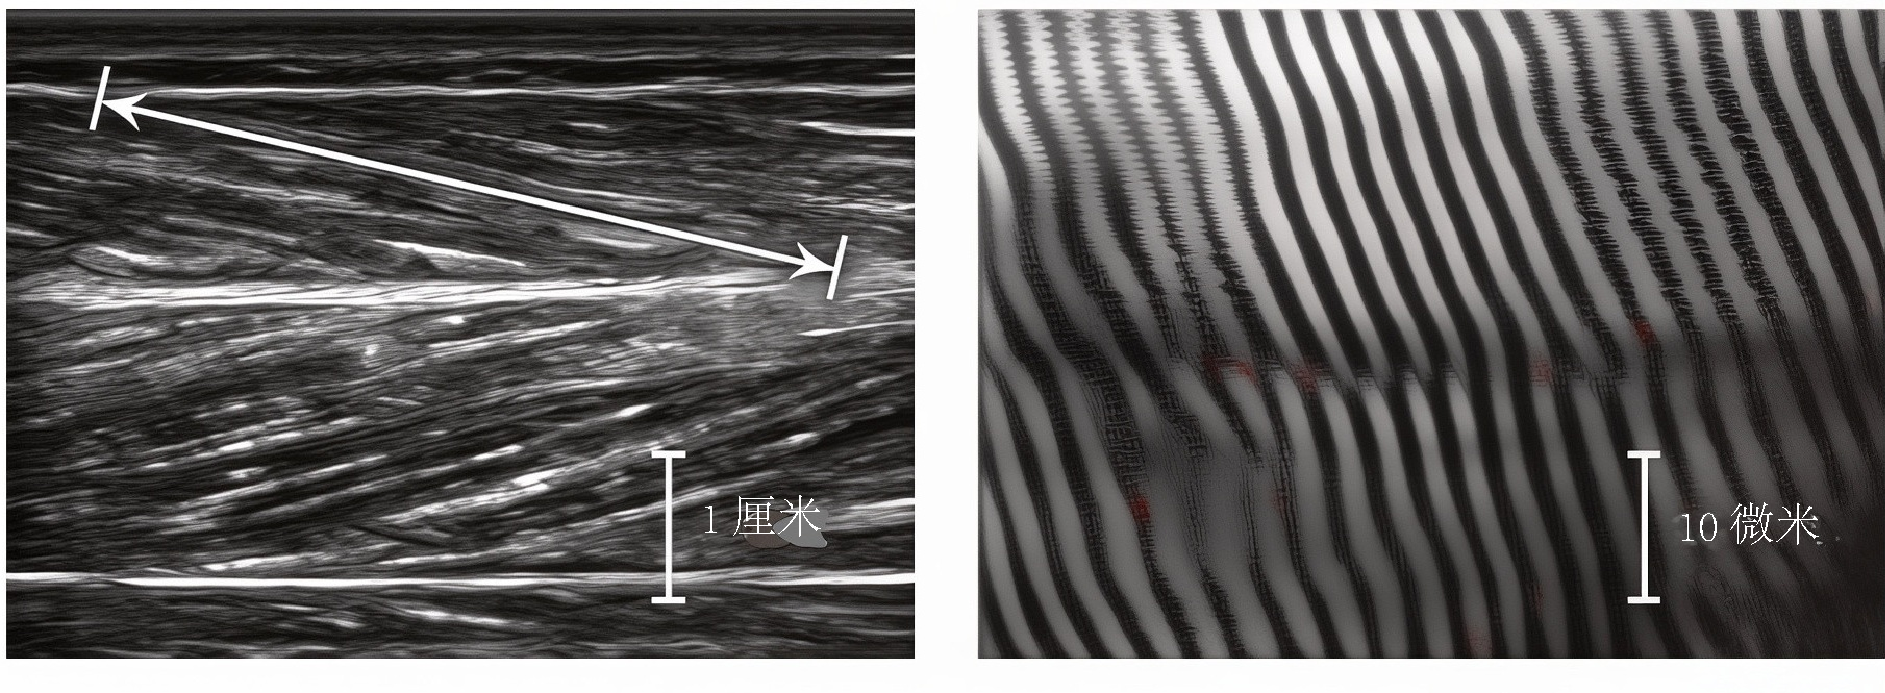
\includegraphics[width=0.75\linewidth]{chap5/5_10}
	\caption{成像技术提供了校准肌肉-肌腱动力学模型所需的数据。
		左图为胫骨前肌纤维的超声图像,可测量纤维长度。
		右图为使用双光子显微内窥镜获得的同一块肌肉的肌节图像,可测量肌节长度。
		图片由 Glen Lichtwark 和 Gabriel Sanchez 提供。 \label{fig:5_10}}
\end{figure}

\begin{equation}
	l_o^M = l^M \times \frac{l_o^S}{l^S}
	\label{eq:5_6}
\end{equation}
%
其中,表示肌节的最佳长度,人体肌肉中估计为 2.7 微米。
有几种技术可以测量整块肌肉的肌节长度。
其中一种方法是激光衍射法,该技术由 Richard Lieber 首创,通过手术暴露肌肉,然后用激光照射肌肉以产生衍射图案\cite{lieber1984sarcomere}。
我的实验室开发了一种侵入性较小的方法\cite{llewellyn2008minimally},使用针头大小的微型内窥镜对体内肌节长度进行成像(图~\ref{fig:5_10},右)。


由于腱膜位于肌肉内部,难以测量,因此在尸体标本或成像实验中难以确定肌腱松弛长度。
在肌肉-肌腱动力学模型中,确定肌腱松弛长度的一种策略是:测量尸体标本的肌纤维长度、肌节长度和关节位置,然后在模型中设定肌腱松弛长度,使肌纤维长度和肌节长度与同一姿势下的尸体测量值相匹配。


如前所述,我们可以通过测量\textit{生理横截面积}和特定张力(公式~\ref{eq:5_4})来估算最大等长肌肉力量。
\textit{生理横截面积}可以通过测量尸体标本的肌肉质量或使用MRI测量肌肉体积来估算,后者更可取,因为老年供体受试者的肌肉可能出现萎缩。
我们可以根据肌肉体积和最佳纤维长度计算\textit{生理横截面积},如下所示:
\begin{equation}
	\text{PCSA} = \frac{\text{muscle volume}}{l_o^M}
\end{equation}
%

在许多针对人体和动物肌肉的实验中,比张力的估算是通过计算最大测量肌肉张力与已知\textit{生理横截面积}(纤维横截面积)的比值(参见公式~\ref{eq:5_4})来实现的。
请注意,文献中报告的\textit{生理横截面积}值实际上可能是严格的几何横截面积,或者可能已经乘以了 $cos_(\phi)$。



\section{肌肉-肌腱动力学的希尔模型}

本节将基于 Hill\cite{hill1938heat}、Wilkie \cite{wilkie1956mechanical} 以及 Ritchie 和 Wilkie (1958) 的研究成果,描述一个广泛使用的肌肉-肌腱动力学模型。
A. V. Hill 在 20 世纪 30 年代进行了开创性的实验,以表征肌肉的力-速度特性。
此后,该模型得到了扩展,以捕捉我们之前描述的肌肉力产生过程中的其他显著特征。
尽管 Hill 只贡献了其中的一部分,但人们仍然习惯称之为“Hill 型模型”。


最流行的希尔型模型由三个部分组成:一个主动收缩元件和一个被动弹性元件,分别代表肌肉的主动和被动力产生特性;以及一个肌腱弹性元件(图~\ref{fig:5_11}A)。
这些元件的符号分别以绿色、橙色和蓝色表示,这些符号借鉴自工程文献。
我们将这三个元件的组合称为肌肉-肌腱执行器。
该模型用简单的元件来表示肌肉和肌腱;生物学的复杂性被提炼为定义这些元件动力学的参数和无量纲曲线。
当然,为了追求计算上易于处理的模型,我们省略了许多生物学细节。


\begin{figure}[!htb]
	\centering
	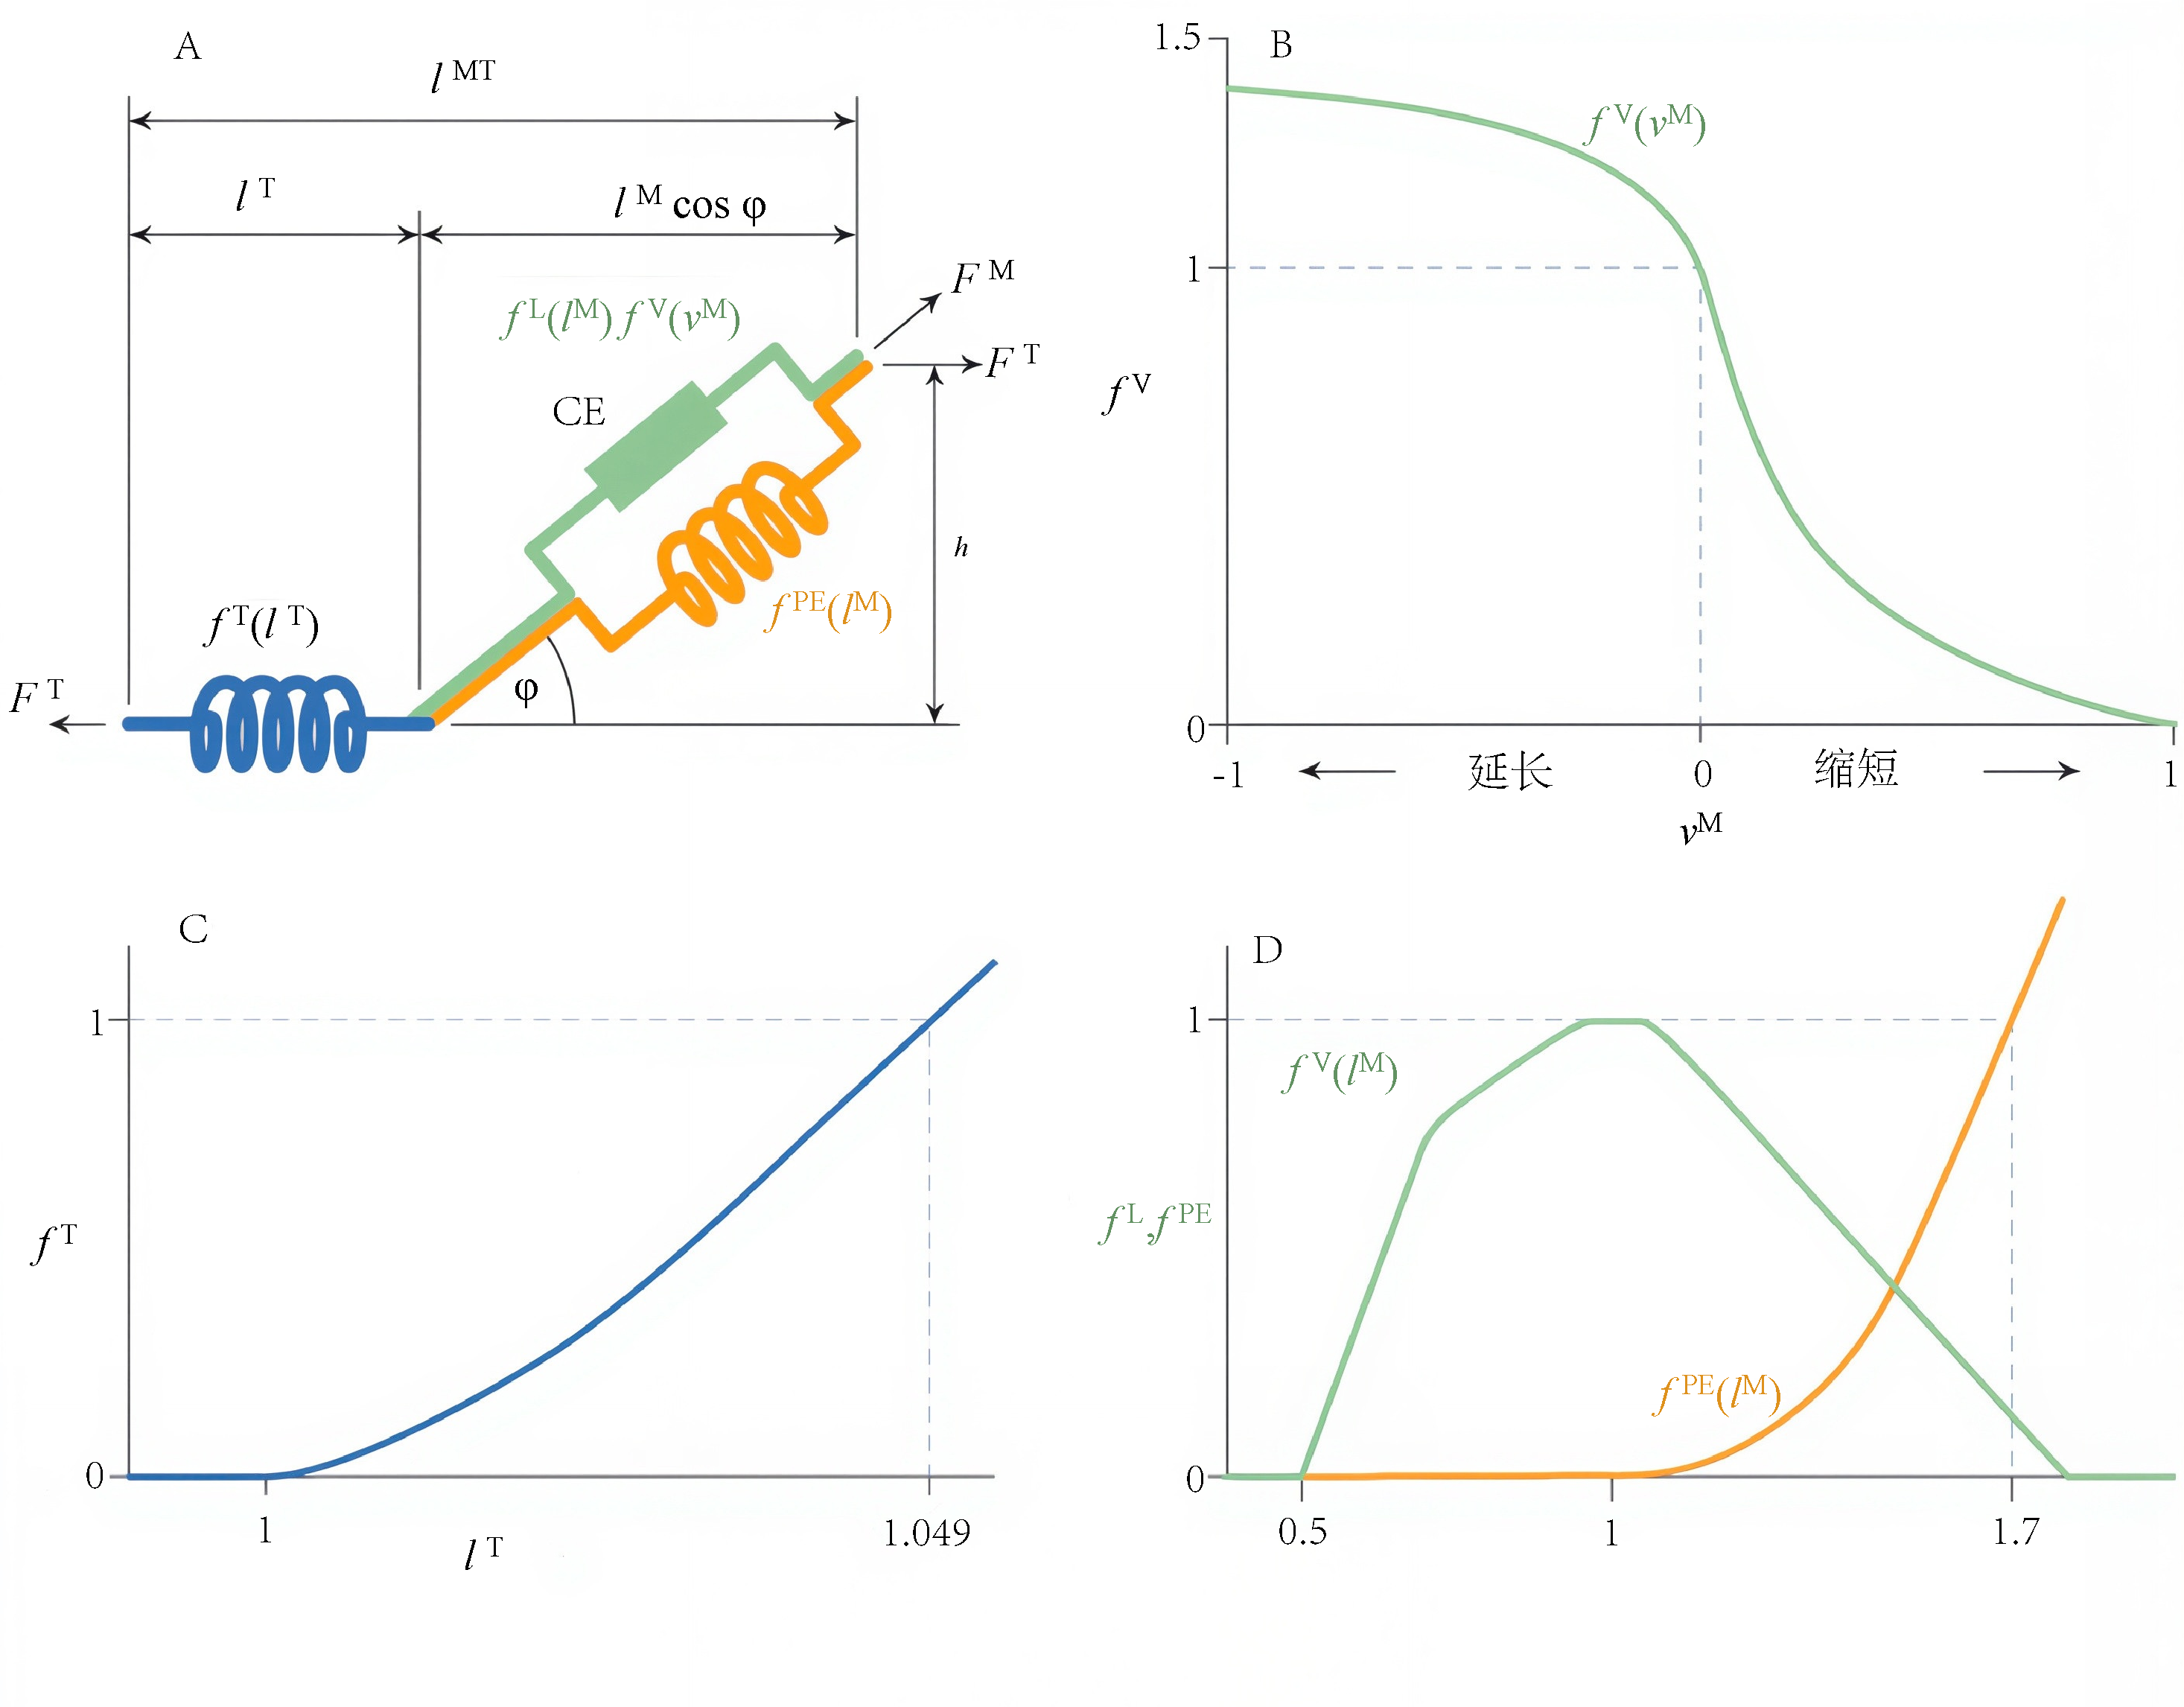
\includegraphics[width=0.85\linewidth]{chap5/5_11}
	\caption{典型的 Hill 型肌肉-肌腱模型示意图(A),以及描述其三个组成部分动力学的相应通用无量纲曲线:力-速度曲线(B)、肌腱力-长度曲线(C),以及主动和被动力-长度曲线(D)。
		图中所示的曲线来自 Millard 等人\cite{millard2013flexing},这些曲线是根据实验数据拟合的,与本文中显示的其他力-长度曲线有所不同。 \label{fig:5_11}}
\end{figure}


该模型常用于全身运动研究,因为它能够提供足够精确的肌肉力量估计,用于研究肌肉在行走和跑步过程中的动作,且计算量不大。
如前所述,肌腱弹性会显著影响肌肉纤维动力学,而肌肉与肌腱的相互作用是该模型的核心特征。
我们假设用一个非线性弹簧来表示肌腱对肌肉两端的影响,在力学上是等效的。
从图~\ref{fig:5_11}A~的示意图中可以看出,肌肉 ($l^M$)、肌腱 ($l^T$) 和肌肉-肌腱执行器 ($l^{MT}$) 的长度关系如下:
\begin{equation}
	l^{MT} = l^M cos(\phi) + l^T
	\label{eq:5_8}
\end{equation}



\section{无量纲曲线}

Hilltype 模型中三个组成部分的力生成特性可以用四条通用的、时不变的曲线来描述,列于表~\ref{tab:5_3},并如图~\ref{fig:5_11}B-D 所示。
一旦我们用肌肉特异性参数对这些曲线进行归一化,它们就变成了无量纲曲线。

\begin{table}[htbp]
	\caption{Hill 型模型使用的 4 条无量纲曲线} \label{tab:5_3} \centering
	\begin{tabular}{ccc} % l水平左居中,c水平居中
		\toprule
		\textbf{模型元素} & \textbf{无量纲曲线} & \textbf{符号}  \\
		\midrule
		主动收缩 & 主动力-长度 &  $f^L(\tilde{l} ^M)$ \\
		\midrule
		 & 力-速度 &  $f^V(\tilde{v} ^M)$ \\
		\midrule
		被动弹性 & 被动力-长度 &  $f^{PE}(\tilde{l} ^M)$ \\
		\midrule
		肌腱弹性 & 肌腱力-长度 &  $f^{T}(\tilde{l} ^T)$ \\
		\bottomrule
	\end{tabular}
\end{table}


通用曲线源自实验测量,反映了肌肉和肌腱的生物学特性。
具体而言,主动力-长度曲线是肌节长度与其激活时产生的力量之间关系的缩放版本(图~\ref{fig:4_6});
双曲线力-速度曲线反映了横桥骑行的动态(图~\ref{fig:4_9});
被动力-长度曲线表示肌肉在拉伸超过其静息长度时产生的力,与其激活无关(图~\ref{fig:4_7});
肌腱力-长度曲线表达了肌腱应变与其应力之间的非线性关系(图~\ref{fig:5_7})。
如图~\ref{fig:5_11}~中出现的归一化变量所示,四条通用的无量纲曲线通过肌腱的松弛长度($l_s^T$)和肌肉的最大等长力($F_o^M$)、最佳纤维长度($l_o^M$)和最大收缩速度($v_\text{max} ^M$)进行缩放。
肌腱力量与肌肉的最大等长力量成比例,因为一般来说,肌肉越强,肌腱就越强,从而避免肌腱衰竭。


缩放和使用无量纲曲线的重要性可以详细讨论,但重点在于,缩放使我们能够分离出模型中每个肌肉和个体独有的部分。
剩下的部分是所有健康肌肉共有的通用部分。



\section{利用刚性肌腱计算肌肉力量}

我们使用图~\ref{fig:5_11}~所示的希尔模型来生成肌肉驱动的运动模拟。
在本节中,我们将介绍构成图~\ref{fig:4_15}中“收缩动力学”模块的数学细节。
具体来说,我们将描述一种在已知肌肉激活度以及肌肉-肌腱执行器的长度和速度的情况下计算肌肉力的策略。
我们假设肌肉激活度已经由激活动力学模型计算出来,因此 $a(t)$ 是已知的。
我们还假设我们知道整个肌肉-肌腱执行器的长度和速度($l^{MT}(t)$ 和 $v^{MT}(t)$)。
但是,我们必须确定肌肉和肌腱的长度。
一旦知道这些长度,我们就可以使用肌肉特定参数以及图~\ref{fig:5_11}~所示的无量纲曲线来计算肌肉产生并通过肌腱传递的力
(请注意,为了简化符号,我们经常省略表示函数依赖时间的“($t$)”,但在本节和下一节中明确显示它,以区分时变量和常数。
还要注意,我们将肌纤维速度定义为缩短速度,以符合肌肉生理学文献和第~\ref{chap:chap4}~章中使用的惯例。
因此,在下面的等式中)。


让我们从一个更简单的问题开始,假设肌腱是刚性的;
然后在下一节中,我们将推广我们的策略,以解释弹性肌腱。
刚性肌腱假设将图~\ref{fig:5_11}A~所示的肌腱弹簧替换为刚性杆(即 $l^T$ 为常数)。
如果肌腱相对于其附着的肌肉较短,则该假设是合理的,在这种情况下,即使受到较大的拉力,肌腱也不会明显拉伸超过其松弛长度(回想一下图~\ref{fig:5_8})。
这样,我们在公式~\ref{eq:5_8}~中剩下 2 个未知数,并且可以将肌肉长度 ($l^M(t)$) 与肌纤维羽状角 ($\phi(t)$) 关联起来,如下所示:
%
\begin{equation}
	l^M(t) = \frac{
				l^{MT}(t) - l^T
			}{
				cos(\phi(t))
			}
	\label{eq:5_9}
\end{equation}

我们有一个方程,但有 2 个未知数。
为了取得进展,回想一下固定高度羽状模型,该模型将肌肉长度和羽状角与图~\ref{fig:5_4}~所示的平行四边形的高度 ($h$) 联系起来,该高度保持不变:
%
\begin{equation}
	h = l^M(t) sin(\phi(t))
	\label{eq:5_10}
\end{equation}

我们可以通过将最佳纤维长度 ($l_o^M$) 和最佳纤维长度处的羽状角 ($\phi_o$) 代入公式~\ref{eq:5_10}~来求解高度 $h$:
%
\begin{equation}
	h = l_o^M sin(\phi_o)
	\label{eq:5_11}
\end{equation}


现在,我们可以求解公式~\ref{eq:5_9}~和~\ref{eq:5_10},得到肌肉长度 ($l^M(t)$) 和羽状角 ($\phi(t)$),其中参数 $h$ 由公式~\ref{fig:5_11}~给出。
我们知道这个系统是可解的,因为独立方程的数量与未知数的数量相同。
将公式~\ref{fig:5_9}~代入公式~\ref{fig:5_10},可以得到羽状角的已知量表达式:
%
\begin{equation}
	\phi(t) = tan^{-1} (
				\frac{h}{
					l^{MT}(t) - l^T
				}
			)
	\label{eq:5_12}
\end{equation}
最后,我们可以使用公式~\ref{eq:5_9}~求解肌肉长度。


肌肉力量 ($F^M(t)$) 可以通过激活值 ($a(t)$)、标准化肌肉长度 ($\tilde{l}^M (t)$) 和标准化肌肉速度 ($\tilde{v} ^M (t)$) 来计算。
%
\begin{equation}
	F^M (t) = 
			F_o^M
			[
				a(t) f^L(\tilde{l}^M (t)) (\tilde{v}^M (t)) 
				+ f^{PE}(\tilde{l}^M (e))
			]
	\label{eq:5_13}
\end{equation}


这里我们将肌肉力的主动和被动分量相加,因为它们是并行作用的。
为了计算肌肉速度 ($v^M (t)$),我们注意到速度是长度的时间导数,并对公式~\ref{eq:5_8}~进行微分:
%
\begin{equation}
	v^{MT} (t) = - v^M(t) cos( \phi(t) )
				 - l^M(t) \dot{\phi}(t) sin( \phi (t) )
				 + v^T (t)
	\label{eq:5_14}
\end{equation}


回想一下,我们假设 $v^{MT}(t)$ 是已知的,而刚性腱假设告诉我们 $v^T(t) = 0$。
因此,公式~\ref{eq:5_14}~中只有 2 个未知数:
肌肉速度 ($v^M(t)$) 和羽状角速度 ($\dot{\phi} (t)$)。
2 个未知数,但只有一个方程。
幸运的是,我们也可以对公式~\ref{eq:5_10}~进行微分,得到与这 2 个变量相关的第二个方程:
%
\begin{equation}
	\hat{\phi (t)} = \frac{v^M (t)}{l^M (t)} tan(\phi (t))
	\label{eq:5_15}
\end{equation}


我们现在将公式~\ref{eq:5_15}~代入公式~\ref{eq:5_14}~来求解肌肉速度,最后使用公式~\ref{eq:5_13}~来计算肌肉力量。



\section{利用柔顺肌腱计算肌肉力量}

当肌腱是柔顺的而不是刚性的时,情况会更加复杂。
在这种情况下,肌腱的长度可以改变,因此 $l^T(t)$ 在公式~\ref{eq:5_9}~中是一个未知数。
处理这个额外未知数的一种策略是将肌肉长度 $l^M(t)$ 定义为状态变量,即在模拟过程中从一个时刻到下一个时刻进行数值积分的量。
该过程的工作原理如下。
我们提供时间零点的肌肉长度的初始值 ($l^M(t)$)、描述肌肉长度变化速率的方程(即其速度 vM(t))以及用于根据肌肉当前长度和速度计算未来短时间长度的数值积分器。
图~\ref{fig:4_15}~中的“收缩动力学”块将具有图~\ref{fig:5_12}~所示的形式。


\begin{figure}[!htb]
	\centering
	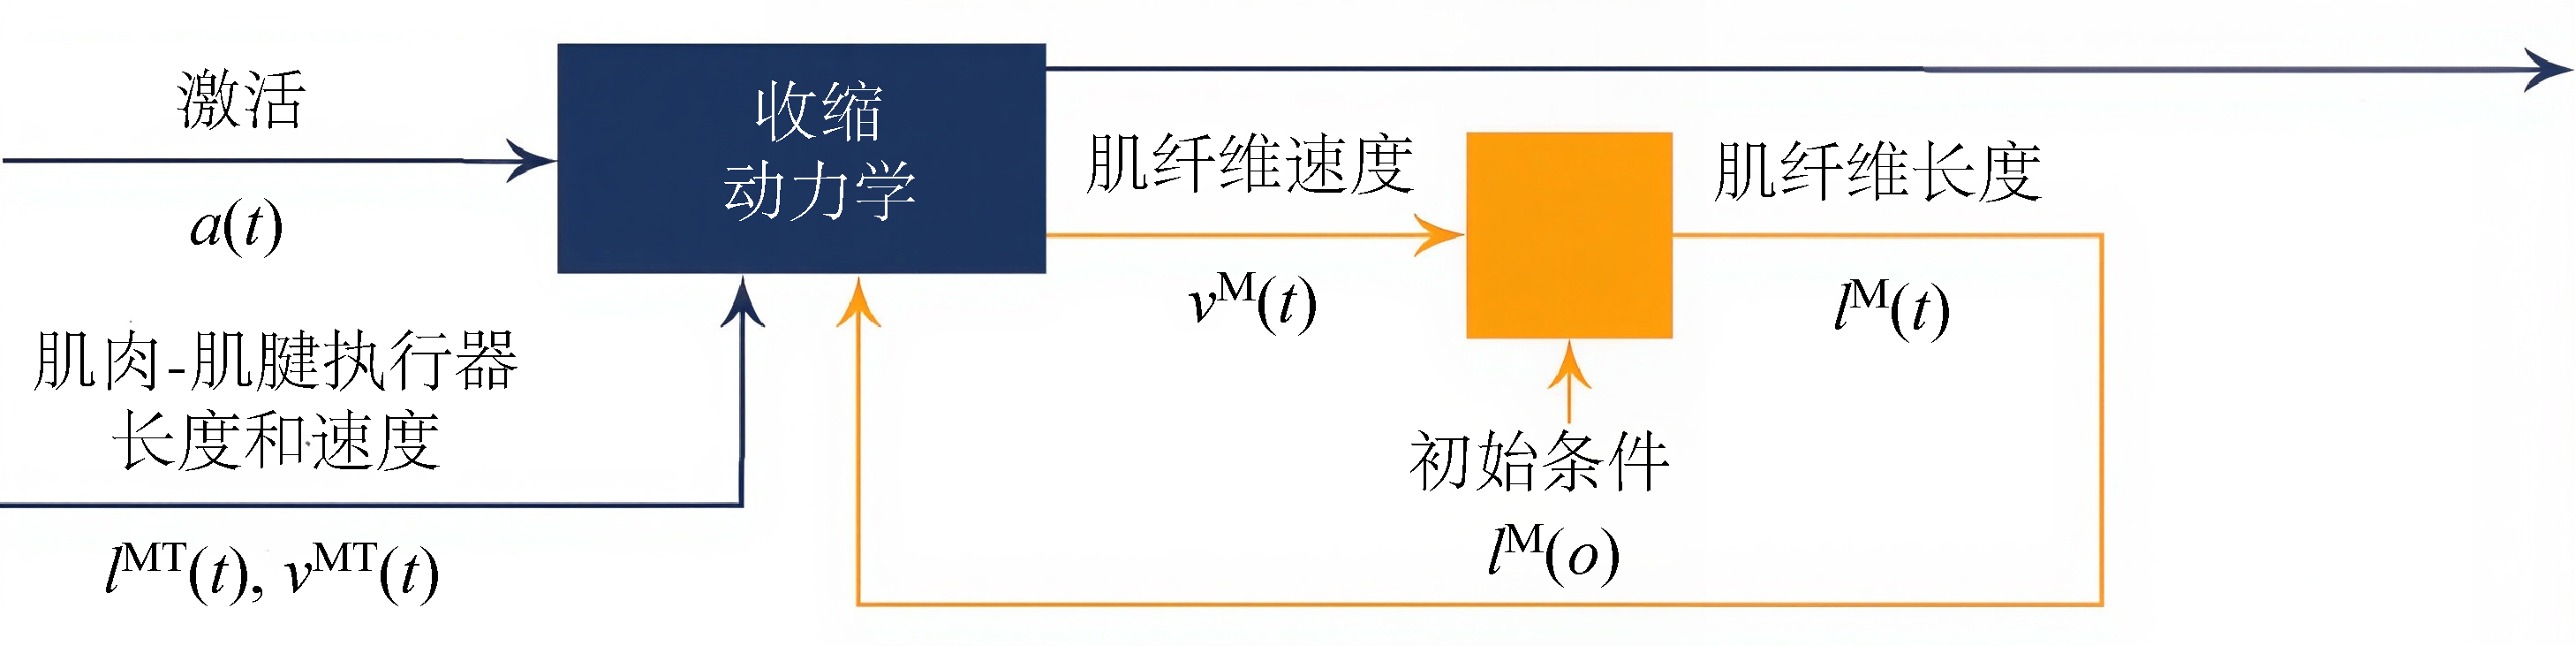
\includegraphics[width=1.0\linewidth]{chap5/5_12}
	\caption{肌纤维长度($l^M(t)$)随时间向前积分,以计算柔顺肌腱的收缩动力学。 \label{fig:5_12}}
\end{figure}


使用简单的数值积分器,我们可以按如下方式计算未来的肌肉长度:
%
\begin{equation}
	l^M (t + \delta t) = l^M (t) - \delta t v^M (t)
	\label{eq:5_16}
\end{equation}
%
其中 $\delta t$ 是每个时间步长推进到未来的时间量(回想一下 $\dot{l} ^M (t) = -v ^M (t)$ )。
通过反复重复此过程,我们最终获得了整个目标时间间隔内的肌肉长度值。使用公式~\ref{eq:5_16}~所示的积分策略(称为欧拉方法)通常需要我们采用较小的时间步长才能获得准确的答案。


现在,我们可以假设肌肉和肌腱无质量且无摩擦,从而推导出 $v^M(t)$ 的表达式,在这种情况下,它们相遇处没有净水平力。
因此,肌肉和肌腱处于平衡状态:
\begin{equation}
	F^T (t) = F^M (t) cos( \phi (t) )
	\label{eq:5_17}
\end{equation}

(因为在图~\ref{fig:5_11}A~中肌腱被限制为保持水平,所以我们可以忽略肌肉产生的力的垂直分量 $F^M(t) sin(\phi(t))$)。
肌腱产生的力 ($F^T(t)$) 可以根据标准化肌腱长度 ($\tilde{l} ^T (t)$) 使用肌腱力-长度曲线计算得出:
%
\begin{equation}
	F^T (t) = F_o ^M [
		f^T
		(
			\tilde{l} ^T (t)
		)
	]
	\label{eq:5_18}
\end{equation}

我们将肌肉和肌腱力的表达式(公式~\ref{eq:5_13}~和~\ref{eq:5_18})代入平衡方程(公式~\ref{eq:5_17})并求解,得到肌肉速度的表达式:
%
\begin{equation}
	\tilde{v} ^M (t) = 
		f_\text{inv} ^V
		(
			\frac{
				f^T (\tilde{l} ^T (T) / cos( \phi (t) ))
				- f^{PE} (\tilde{l} ^M (t))
			}{
				a(t) f^L ( \tilde{l}^M (t) )
			}
		)
	\label{eq:5_19}
\end{equation}
%
其中 $f_\text{inv} ^V$ 是力-速度曲线的倒数(即,它描述肌肉速度作为力的函数)。
请注意,公式~\ref{eq:5_19}~有 4 个数值奇异点,在模拟过程中必须避免:
当羽状角接近 90 度时、当激活度接近零时、当纤维长度达到主动力-长度曲线接近零时,以及当力-速度曲线不可逆时。
可以通过对相应变量引入约束来避免这些奇异点,例如,防止羽状角超过小于 90 度的某个上限。


上述方法用于估算几乎所有肌肉驱动运动模拟中的肌肉和肌腱力量。
该方法的价值在于,它使我们能够在估算每块肌肉产生的力量时,考虑其激活程度、纤维长度和纤维速度。
然而,其他方法也同样有用,我们将在下文中进行介绍。



\section{肌肉力量产生的其他模型}

我们重点关注希尔型模型,因为它广泛应用于运动模拟,包括本书介绍的运动模拟。
然而,希尔型模型未能捕捉到一些现象。
例如,该模型忽略了短程刚度(描述肌肉对长度小幅快速扰动产生的与速度无关的抵抗力);忽略了力量增强(即拉伸后肌肉最大等长收缩力的立即增加);以及对温度和疲劳的依赖性。
此外,虽然希尔型模型能够很好地表示肌肉在最大活动状态下,长度和速度变化引起的肌肉力量变化,但它对于次最大活动状态的准确性较低\cite{millard2013flexing}。
在科学研究中使用希尔型模型时,必须考虑这些局限性。


其他肌肉模型也已开发出来,有的更简单,有的更复杂。
一种简单的肌肉力建模策略是,用一个扭矩执行器(一种具有生理学特性的马达)来表示关节上所有肌肉产生的总力矩。
该执行器的最大扭矩可以表示为关节角度的函数,该角度由实验确定,但无法计算单个肌肉的力。
正如我们将看到的,该模型足够简单,可用于大规模优化问题,同时仍能产生与人类运动非常相似的模拟结果。


当需要更详细的信息来解答特定问题时,也有一些肌肉模型可以提供这些信息。
一个著名的例子是基于安德鲁$\cdot$赫胥黎\cite{huxley1957muscle}的研究,其中明确地模拟了肌肉收缩的滑动丝机制。
这个赫胥黎型模型使用以下形式的偏微分方程来描述力的产生:
%
\begin{equation}
	\frac{\partial n(x,t)}{\partial t}
	- v(t) \frac{\partial n(x,t)}{\partial x}
	= f(x)
	- ( f(x) + g(x) ) n(x,t)
	\label{eq:5_20}
\end{equation}
%
其中 $n(x,t)$ 是描述参与横桥循环的肌动蛋白和肌球蛋白比例的概率密度函数;
$x$ 和 $t$ 是距离和时间的独立变量;
$v(t)$ 是半肌节的缩短速度;
函数 $f(x)$ 和 $g(x)$ 分别表示横桥形成和断裂的速率。
使用该模型的主要挑战是确定模型中许多参数的适当值,因为我们对这些量在不同物种和不同肌肉之间的变化知之甚少。
尽管如此,该模型捕捉到了上述一些希尔型模型未能捕捉到的效应。
横桥模型通常用于研究单块肌肉的动力学。


有限元模型提供了另一种选择。
在有限元模型中,肌肉被划分为许多小单元(数量级达数千个),每个单元由一组描述组织行为的方程控制。
有限元模型是工程应用(例如飞机设计)的最新方法,毫无疑问,它们比我们在本章中推导的简单方程具有更高的精度。


但更强大的计算能力是有代价的:
有限元模型的求解时间比希尔型模型长数百倍。
尽管计算负担较大,有限元模型仍能有效地模拟纤维长度不一、应变不均匀且横向传递张力的肌肉(图~\ref{fig:5_13})。
最终,您必须在模型提供的细节量与其针对具体应用的分析可处理性之间找到适当的平衡。


\begin{figure}[!htb]
	\centering
	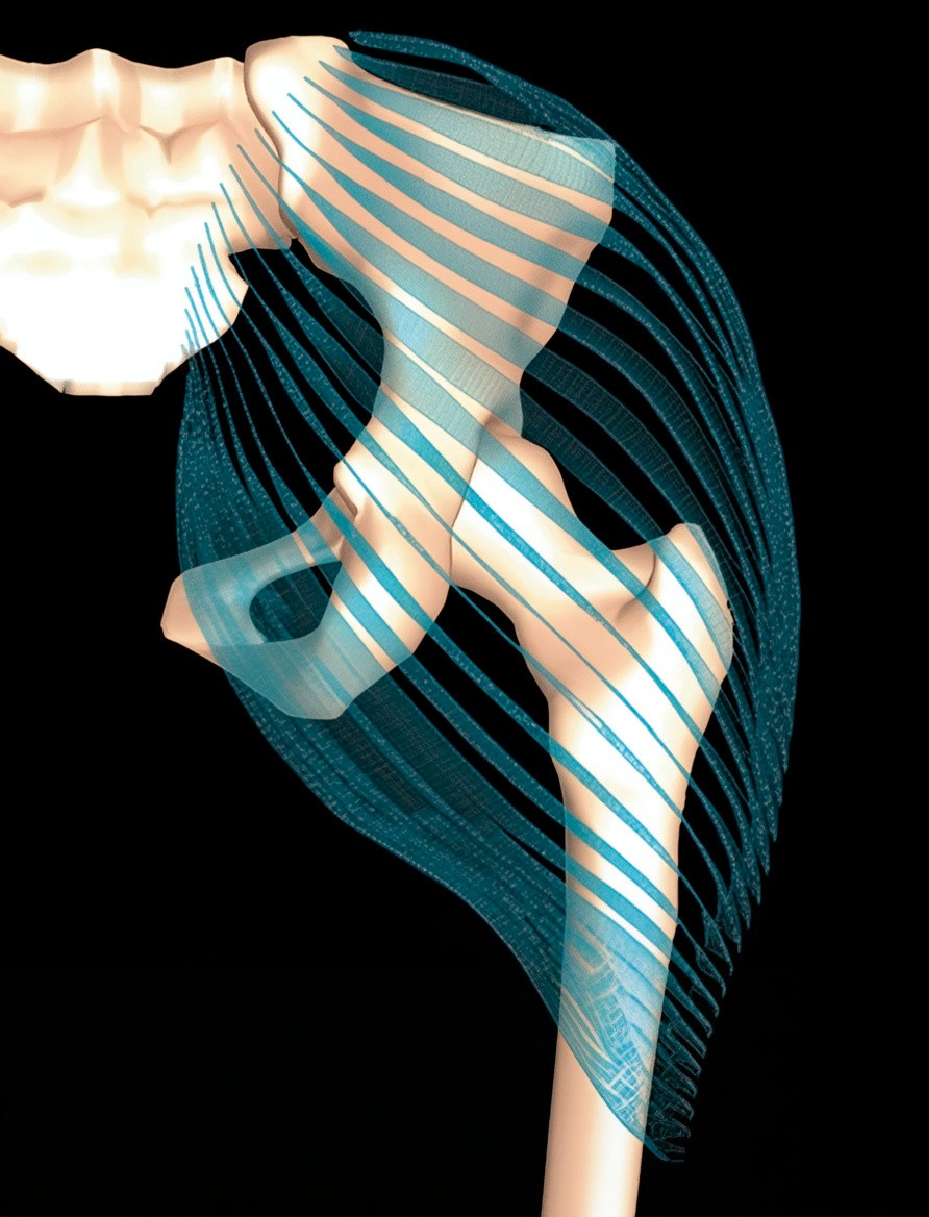
\includegraphics[width=0.4\linewidth]{chap5/5_13}
	\caption{Blemker\cite{blemker2005three}的臀大肌模型。
		有限元模型提供了肌肉结构的详细特征,并可以计算内部肌肉和肌腱的应变。 \label{fig:5_13}}
\end{figure}


由于许多肌肉参与运动的协调和控制,因此,对大量肌肉进行模拟对于研究步行和跑步等活动至关重要。
本章讨论的模型使我们能够仅使用少量计算资源一次模拟数十块肌肉。
我们将在第~\ref{chap:chap10}~至~\ref{chap:chap12}~章中展示我们的计算能力,以生成肌肉驱动的运动模拟。




\chapter{肌肉骨骼几何学} \label{chap:chap6}



\chapter{运动量化} \label{chap:chap7}





\chapter{逆动力学} \label{chap:chap8}

任何作用力都会产生一个大小相等的反作用力。

\begin{flushright}
	——艾萨克$\cdot$牛顿爵士
\end{flushright}

\begin{figure}[!htb]
	\centering
	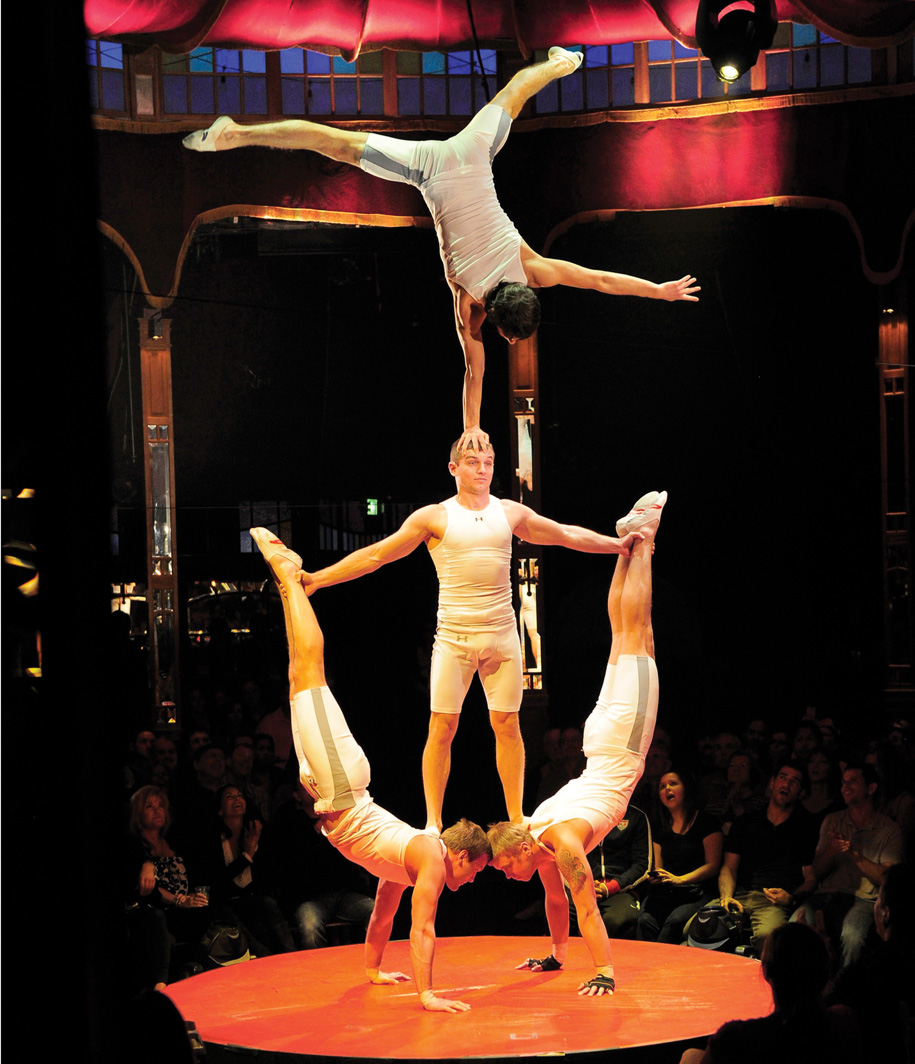
\includegraphics[width=1.0\linewidth]{chap8/8_0}
	% 加星号(*)表示不加编号
	\caption*{ \label{fig:8_0}}
\end{figure}


我母亲75岁时,几乎已经无法行走。
她的右膝每走一步都疼痛难忍,爬楼梯更是不可能。
她想和我的孩子们一起玩,却跟不上他们。
无法行走不仅限制了她参与生活,还给她带来了心理上的创伤。
膝盖 X 光检查显示,她患有严重的骨关​​节炎,这是一种影响美国超过3000万人的退行性关节疾病(图~\ref{fig:8_1})。


\begin{figure}[!htb]
	\centering
	\includegraphics[width=0.4\linewidth]{chap8/8_1}
	\caption{膝盖 X 光片显示骨关节炎的迹象。
		请注意,膝盖内侧的骨头相互接触(见箭头);
		外侧保留了更多的软骨,表现为股骨和胫骨之间的间隙。
		图片由Julie Thompson-Kolesar提供。 \label{fig:8_1}}
\end{figure}


骨关节炎是由于覆盖骨骼末端的软骨表面磨损而引起的。
软骨很滑,没有痛觉,因此它是一种极好的材料,可以让我们的关节自由活动,而我们却感觉不到任何疼痛。
然而,当软骨磨损时,会暴露出下面的骨骼,而骨骼对压力极其敏感,会产生更大的摩擦力,导致关节感到疼痛和僵硬。


膝盖负荷过重会导致磨损,最终引发骨关节炎,然而,如果不进行手术来安装传感器,就无法测量关节内的负荷。
目前只有少数勇敢的患者因其他原因接受了手术,才得以实现这一目标。
因此,我们通常采用其他方法来估算关节内的负荷。
求解逆动力学问题可以提供一些估算关节接触负荷所需的信息,这是理解生物关节失效原因的关键一步。


当工程产品发生故障时,法医工程师会努力查明故障的根本原因,并最终追究相关人员的法律责任。
例如,律师事务所会聘请精通生物力学的法医工程师,评估车辆碰撞后伤害索赔的合法性。
轮胎滑痕等物证可以用来估算碰撞过程中的力和加速度。
事故重建过程就是逆问题的一个例子,因为人们会使用间接观测来研究无法直接测量的现象。


在第~\ref{chap:chap7}~章中,我们介绍了逆运动学问题,其中一个例子是通过测量安装在皮肤上的光学标记在全局参考系中的位置来确定受试者骨骼的姿态。
在那一章中,我们的目标很有限;
我们只是在回答这个问题:发生了什么?
换句话说,为了产生观察到的标记轨迹,必须存在哪些关节角度?
在本章中,我们将深入探究:是什么导致了这一切?
具体来说,是什么力和力矩导致了观察到的运动?


从运动学中确定力和力矩的过程称为逆动力学。
它与逆运动学不同,因为我们感兴趣的是产生运动的力,而不仅仅是运动本身。
它也不同于正向动力学,在正向动力学中,我们预测当指定的力施加到系统上时将产生的运动。


逆动力学问题可以通过几种方法求解。
通常,如果可以测量地面反作用力,我们会使用测量数据,因此我们将首先简要讨论测量这些力的技术。
然后,我们将展示一个详细的例子,说明如何计算深蹲过程中的关节力矩。
在这个例子中,我们从地面向上进行计算,使用地面反作用力的测量数据,并将这些信息通过腿部关节向上传递。
如果我们拥有所有身体部位运动的可靠测量数据,也可以从上向下进行计算。


请注意,本章计算的力并非生物关节中实际测量的力。
为了计算关节接触载荷,我们还必须估算肌肉施加的力。
这是一个非同小可的问题,将是第~\ref{chap:chap9}~章的重点。
目前,只需注意,相同的运动和外力可能会因肌肉协调策略的差异而产生不同的测量结果,从而产生不同的关节接触载荷(但逆动力学问题的解是相同的)。


有趣的是,如果我们能够获取地面反作用力以及所有身体部位的运动,就能得到一个超定方程组。
在这种情况下,我们可以利用这些额外的信息来最小化测量误差的影响,这一策略与第~\ref{chap:chap7}~章中描述的约束逆运动学算法相呼应。
本章最后将以一个例子来结束,该例子展示了如何利用逆动力学分析来评估膝关节骨关节炎患者的非手术治疗。
如果我早 20 年想到这个方法,或许就能帮助到我的母亲。



\section{测量外力}

牛顿的三大运动定律,最早发表于他 1687 年出版的里程碑式著作《自然哲学的数学原理》中。
牛顿第二定律是迄今为止最重要的方程之一;
安德鲁$\cdot$莫特于 1729 年从拉丁文原文翻译了该定律,其表述如下:


定律二:运动的改变总是与所施加的动力成正比;
并且是沿着施加该力的直线方向进行的。


换句话说,粒子动量的变化率等于作用力的矢量和,方向与作用力的方向一致。
牛顿第二定律现在通常被称为 $\underline{F} = m \underline{a}$,其中$\underline{F}$是作用于物体的所有力的矢量和,$m$是物体的质量,$\underline{a}$是其质心的(线性)加速度。
这个版本遵循原始版本,前提是物体的质量在运动过程中保持不变,这在大多数应用中都是合理的(火箭技术是一个显著的例外)。
莱昂哈德$\cdot$欧拉后来将牛顿定律扩展到旋转运动。
欧拉第二定律告诉我们,物体绕其质心的角动量的变化率等于作用于该点的所有矩之和。
(有关正式的数学表述,请参见下面的公式~ 8.6。)


如果已知每个身体部位的质量和加速度,我们可以使用牛顿定律和欧拉定律来确定施加在每个身体上的力和力矩。
根据所研究的运动,可能会有外力作用于主体,例如重力、空气阻力或地面反作用力。
这些外力出现在主体的自由体图中,必须进行测量或估算。
在大多数人体运动情况下,忽略空气阻力并使用重力加速度 $g = 9.81 m/s^2$ 来计算重量是合理的。
我们通常倾向于尽可能测量地面反作用力和其他接触力,以提高计算的准确性,如下所示。


19 世纪末,Étienne-Jules Marey 和他的学生 Gaston Carlet 设计了第一批用于测量足部与地面接触力的装置。
通过将压力传感器嵌入鞋底,Marey 和 Carlet 能够估算出步态过程中足部与地面之间施加的力。
Carlet 的博士论文首次报告了步行过程中地面反作用力特有的双峰垂直分量,该论文发表于 1872 年——同年,利兰$\cdot$斯坦福聘请 Eadweard Muybridge 确定马匹在小跑时是否完全腾空(见图~\ref{fig:7_1})。
我发现,现代生物力学最重要的两个定量工具竟然是由两位几乎完全不知道对方在做什么的研究人员(Carlet 和 Muybridge)同时开发的,这真是令人惊叹。


在现代实验中,地面反作用力是使用一个或多个测力板来测量的:由负载传感器支撑的平坦刚性平台(图~\ref{fig:8_2})。
负载传感器包含应变计或压电晶体,可将平台的微小位移转换为电压。
虽然测力板有点像普通的弹簧式体重秤,但它们在精度、速度和数据丰富度方面存在很大差异。
由于地面反作用力变化迅速,尤其是在脚着地时,因此数据通常以每秒数千次测量的速率收集。
测力板的每个角附近通常都有一个负载传感器,每个负载传感器测量应变并报告沿三个正交轴的力。
因此,测力板有 12 个独立的力测量值,而不是像体重秤那样只有一个,这些测量值可以组合起来计算相对于测力板原点的合力和力矩。


\begin{figure}[!htb]
	\centering
	\includegraphics[width=0.7\linewidth]{chap8/8_2}
	\caption{测力台测量施加于地面和受试者之间的力和力矩,统称为地面反作用力。压力中心 (COP) 和“自由力矩” ($\underline{T}$) 可以通过合力 ($\underline{F}$) 和总力矩 ($\underline{M}$) 计算得出。 \label{fig:8_2}}
\end{figure}



\section{压力中心}

足底的压力分布不均匀(图~\ref{fig:8_3})。
这种分布的压力可以表示为施加于压力中心点的等效合力。
我们可以使用以下矩等效方程来确定压力中心:

\begin{figure}[!htb]
	\centering
	\includegraphics[width=1.0\linewidth]{chap8/8_3}
	\caption{行走时足部压力分布\cite{pataky2012gait}。 \label{fig:8_3}}
\end{figure}

\begin{equation}
	\underline{M} = \underline{r} \times \underline{F} + \underline{T}
	\label{eq:8_1}
\end{equation}
%
其中,$\underline{M}$表示测力板原点处的力矩,$\underline{r}$表示从原点到压力中心的矢量,$\underline{F}$表示合成的地面反作用力,$\underline{T}$表示在压力中心施加力时产生等效系统所需的力矩(图~\ref{fig:8_2})。
在公式~\ref{eq:8_1}~中,我们有 3 个独立方程(分别表示 $M_x$、$M_y$ 和 $M_z$),但有 6 个未知数:
矢量的 3 个分量和力矩的 3 个分量。
我们注意到压力中心保持在测力板表面($r_z = 0$),并且表面摩擦只能产生绕垂直轴的力矩($T_z$,也称为“自由力矩”),从而得到了三个附加方程。
虽然可以想象绕其他两个轴的力矩,但只有将人的脚粘在测力板上才能观察到这些力矩。
这样,脚粘的受试者才有可能产生向下的地面反作用力,从而绕其他两个轴产生力偶。


在没有粘脚的情况下,我们可以将$r_z = T_x = T_y = 0$代入公式~\ref{eq:8_1},并求解其余未知数。
我们得到压力中心相对于力板原点的位置($\underline{r}$)和自由矩($T_z$)的以下表达式:
%
\begin{equation}
	\underline{r} = 
		\begin{bmatrix}
			- M_y / F_z \\
			M_x / F_z \\
			0
		\end{bmatrix}
	\label{eq:8_2}
\end{equation}

\begin{equation}
	T_z = M_z - r_x F_y + r_y F_x
	\label{eq:8_3}
\end{equation}


在验证数据处理算法时,计算并可视化压力中心非常有用;
如果压力中心位于足迹之外,则表明测力板和运动捕捉系统之间存在校准误差。
通常,将作用于足部的力和力矩转换为压力中心,也更容易理解。
请注意,当地面反作用力 ($F_z$) 的法向分量趋近于零时,公式~\ref{eq:8_2}~中的表达式会变得病态,因此在足部触地和足尖离地附近计算出的压力中心将不可靠。



\section{逆动力学算法}

动力学分析考虑物体的运动(运动学)以及导致该运动并由该运动产生的力(动力学)。
在本节中,我们将考虑一个典型的逆动力学问题:给定一个受试者的代表性模型、受试者随时间变化的关节运动学以及施加于受试者的外力测量值,求出产生给定运动所必需的净关节力和力矩。
简而言之,我们将力学定律应用于模型中的每个身体部位,并计算作用于每个关节的内部力和力矩。
关节角度通常使用逆运动学算法(第~\ref{chap:chap7}~章)根据光学标记轨迹估算,然后对其进行平滑和微分以获得角速度和角加速度。
无需测量外力即可进行逆动力学分析,但我们将把这方面的讨论推迟到本章的后面。
为了演示一个简单的逆动力学算法,我们将计算图~\ref{fig:8_4}~所示的深蹲过程中的净关节力和力矩。


\begin{figure}[!htb]
	\centering
	\includegraphics[width=1.0\linewidth]{chap8/8_4}
	\caption{用于研究深蹲的实验装置(左)和近似矢状面模型(右)。
		逆动力学分析根据每个身体部位的质量、惯性、几何形状和运动学参数(位置、速度和加速度)(以及外力,如有)计算每个关节处的净力和力矩。 \label{fig:8_4}}
\end{figure}


在继续之前,值得考虑一个重要问题:如何为特定研究选择合适的模型,具体来说,图~\ref{fig:8_4}~所示的简单模型是否适合研究深蹲。
一般来说,适当的模型保真度(即模型代表现实的程度)取决于所研究的问题。
重要的是要认识到,更详细的模型并不一定更好。
选择模型的目标是最大化模型的效用,这通常涉及最小化其复杂性,以使模拟结果不被无关细节所污染。
这一目标呼应了爱因斯坦 1934 年的论文《论理论物理方法》中的以下智慧:


不可否认的是,所有理论的最高目标都是使不可简化的基本要素尽可能简单、尽可能少,同时又不必放弃对单一经验数据的充分表示。


爱因斯坦谈论的是理论物理学和实验物理学之间的关系,但这里也秉持着同样的理念:
我们倾向于那些复杂程度最低、同时能够解释实验观测结果并以足够高的精度产生所需输出的模型。
正如统计学家乔治$\cdot$博克斯和诺曼$\cdot$德雷珀的名言所说:“所有模型都是错误的,但有些模型是有用的。”


一个特定模型是否有用,而不是仅仅有误,取决于它的使用环境。
例如,在模拟太阳系中的行星轨道或预测行星际航天器的轨迹时,将火星建模为点质量可能是合理的,但这样的模型不足以研究火星的天气模式或模拟航天器在那里着陆。
相反,在轨道力学研究中使用详细的行星模型会增加建模的复杂性和计算工作量,而不会增加结果的价值。
回到生物力学领域,我们注意到,一些 OpenSim 软件的新用户最初认为他们应该始终使用具有数十个自由度的全身模型,而实际上一个简单得多的模型就可以告诉他们关于他们感兴趣的特定主题所需的一切信息。
只能屈曲和伸展的单自由度膝关节模型可能适合研究膝关节伸展力矩如何随跑步速度而变化,而分析骨关节炎患者的额平面力矩则需要具有更多自由度的更详细的膝关节模型。



\section{具有地面反作用力的逆动力学}


在本节中,我们将使用图~\ref{fig:8_4}~所示的平面模型,对双腿下蹲的某一瞬间进行逆动力学分析。
该模型由四个刚体组成,它们通过三个旋转(销)关节连接,分别代表踝关节、膝关节和髋关节。
我们假设关节角度、角速度和角加速度已通过先前求解逆运动学问题获得。
我们进一步假设受试者的身体是对称的,并且任何超出矢状面的运动都可以忽略不计。
我们将左右脚组合成一个刚体(“脚”),假设其质量可忽略不计,并在地面上保持静止。
左右小腿也组合成一个刚体,其质量和惯性分别代表两个小腿;左右大腿也以类似的方式组合。
我们将头部、手臂和躯干(HAT)建模为一个刚体。
我们假设模型的每个身体部位都经过适当缩放,以匹配受试者相应身体部位的尺寸和质量特性。
在实践中,模型参数(例如长度、质量和惯性)可以通过结合直接测量、已发表的人体测量表、照片、医学图像以及其他测量和估算技术来确定。
我的团队开发的 OpenSim 模型包含这些参数的值,这些值可以缩放以代表特定个体。
我们的模型可免费获取,可从本书网站访问。


在这个简单的例子中,我们将从脚部开始,利用运动定律,借助一系列自由体运动图,计算从脚踝开始的每个关节所受的净力和力矩。
目前,我们假设地面反作用力已知。
对于像这样的简单模型,绘制自由体运动图并进行手算的策略已经足够;
在实践中,我们通常使用与下文类似的算法的软件实现。


我们假设尺寸和地面反作用力已知,并且双足无质量且静止不动。
因此,在足部自由体受力分析图(图~\ref{fig:8_5})中唯一未知的就是施加于踝关节的力和力矩。
注意,根据牛顿第三运动定律,作用于小腿踝关节的力和力矩必须大小相等、方向相反。
我们习惯于在较近端的小腿上绘制这些矢量对的正方向,在较远端的小腿上绘制这些矢量对的负方向。
例如,图~\ref{fig:8_5}~中的 $F_{x_1}$ 矢量指向 -X 方向,则小腿自由体受力分析图(图~\ref{fig:8_6})中对应的矢量将指向 +X 方向。


\begin{figure}[!htb]
	\centering
	\includegraphics[width=0.7\linewidth]{chap8/8_5}
	\caption{模型足部段的自由体受力图如图~\ref{fig:8_4}~所示。 \label{fig:8_5}}
\end{figure}


\begin{figure}[!htb]
	\centering
	\includegraphics[width=0.7\linewidth]{chap8/8_6}
	\caption{图~\ref{fig:8_4}~所示模型小腿段的自由体图。
		自由体图中身体段的姿势无需与其在研究活动中的姿势一致。
		虽然数学上无关紧要,但我们以这个方便的标准姿势绘制小腿段,其中 1 介于 0 到 90 度之间。 \label{fig:8_6}}
\end{figure}


我们可以使用牛顿第二定律及其旋转类似物来求解 $F_{x_1}$、$F_{y_1}$ 和 $T_1$。
首先,我们将力相加,并在 X 方向应用牛顿第二定律来计算 $F_{x_1}$:
%
\begin{equation}
	\sum F_X = m_0 \ddot{x}_0
	\label{eq:8_4a}
\end{equation}


\begin{equation}
	F x_g - F x_1 = 0
	\label{eq:8_4b}
\end{equation}


\begin{equation}
	F_{x_1} = F_{x_g}
	\label{eq:8_4c}
\end{equation}
%
其中 $m_0$ 是足部的质量,$\ddot{x}_0$是其质心的水平加速度,我们假设两者都为 0。
接下来,我们将 Y 方向上的力相加,计算出 $F_{y_1}$:
%
\begin{equation}
	\sum F_y = m_0 \ddot{y}_0
	\label{eq:8_5a}
\end{equation}

\begin{equation}
	F y_g - F y_1 = 0
	\label{eq:8_5b}
\end{equation}

\begin{equation}
	F y_1 = F y_g
	\label{eq:8_5c}
\end{equation}

最后,我们解出$T_1$。
我们上面提到的旋转类似物 $\underline{F} = m \underline{a}$,在平面系统中计算物体上任意点$P$的矩时,具有以下一般形式:
%
\begin{equation}
	\sum M_p = 
		I \ddot{\theta} + 
			( \underline{r}^P \times m \underline{a} ) \cdot \hat{z}
	\label{eq:8_6}
\end{equation}
%
其中,$\sum M_p$ 是关于点 $P$ 的力矩之和,$I$ 是物体绕其质心 (COM) 的转动惯量,$\ddot{\theta}$ 是物体的角加速度, 是从点 $\underline{r} ^P$ 到质心的矢量,$m$ 是物体的质量,$\underline{a}$ 是物体质心的线加速度。
由于质量与加速度的乘积是力,我们可以将公式~\ref{eq:8_6}~右边的第二项解释为力矩在旋转轴上的投影(正如我们在公式~\ref{eq:6_4}~中看到的那样)。


无论计算哪个点的矩,都会得到等效的方程组。
为简单起见,我们通常计算重心的矩,使得公式~\ref{eq:8_6}~中的叉积为零(具体来说,使得 $\underline{r} ^P = \underline{0}$ )。
然而,我们假设足部无质量且静止。
因此,公式~\ref{eq:8_6}~的右边始终为零,我们可以假设重心位于任意位置。
为方便起见,我们将踝关节的矩相加:
%
\begin{equation}
	\sum M_A = 0
	\label{eq:8_7a}
\end{equation}

\begin{equation}
	F x_g b - F y_g l - T_1 = 0
	\label{eq:8_7b}
\end{equation}

\begin{equation}
	T_1 = F x_g b - F y_g l
	\label{eq:8_7c}
\end{equation}

方程~\ref{eq:8_4c}c、\ref{eq:8_5c}c~和~\ref{eq:8_7c}c~包含一个线性方程组,可用于在给定 $l$、$h$、$F_{x_g}$ 和 $F_{y_g}$ 的情况下计算 $F_{x_1}$ 、$F_{y_1}$ 和 $T_1$ 。


现在,我们对小腿段(图~\ref{fig:8_6})重复该过程,其中,假设施加于踝关节的力和力矩($F_{x_1}$、$F_{y_1}$ 和 $T_1$)在上一步中已知,而施加于膝盖的力和力矩($F_{x_2}$、$F_{y_2}$ 和 $T_2$)现在是未知数。
我们首先根据踝关节的运动学特性($\theta_1$、$\dot{\theta}_1$ 和 $\ddot{\theta}_1$)计算重心的加速度($\ddot{x}_1$ 和 $\ddot{y}_1$),并注意踝关节中心是静止的:
%
\begin{equation}
	x_1 = r_1 c \theta_1
	\label{eq:8_8a}
\end{equation}

\begin{equation}
	\dot{x}_1 = - r_1 s \theta_1 \dot{\theta}_1
	\label{eq:8_8b}
\end{equation}

\begin{equation}
	\ddot{x}_1 = - r_1 ( s \theta_1 \ddot{\theta}_1 + c \theta_1 \dot{\theta}_1^2 )
	\label{eq:8_8c}
\end{equation}

\begin{equation}
	y_1 = r_1 s \theta_1
\end{equation}

\begin{equation}
	\dot{y}_1 = r_1 c \theta_1 \dot{\theta}_1
	\label{eq:8_9b}
\end{equation}

\begin{equation}
	\ddot{y}_1 = r_1 ( c \theta_1 \ddot{\theta_1}  -  s \theta_1 \dot{\theta}_1^2 )
	\label{eq:8_9c}
\end{equation}
%
其中,为了方便记号,我们使用了 $s \theta_1 \triangleq  sin (\theta_1)$ 和 $c \theta_1  \triangleq  cos (\theta_1)$。
现在我们在 X 方向应用牛顿第二定律来计算 $F_{x_2}$:
%
\begin{equation}
	\sum F_X = m_1 \ddot{x}_1
	\label{eq:8_10a}
\end{equation}

\begin{equation}
	F_{x_1} - F_{x_2} = 
		- m_1 r_1 
		(
			s \theta_1 \ddot{\theta}_1 + 
			c \theta_1 \dot{\theta}_1^2
		)
	\label{eq:8_10b}
\end{equation}
%
并再次沿 Y 方向计算 $F_{y_2}$:
\begin{equation}
	F y_1 - F y_2 - m_1 g  =  
		m_1 r_1
		(
			c \theta_1 \ddot{ \theta }_1 -
			s \theta_1 \dot{ \theta }_1^2
		)
	\label{eq:8_11}
\end{equation}

最后,我们对 COM 的矩求和以获得 $T_2$ 的表达式:
%
\begin{equation}
	\begin{aligned}
		T_1 - T_2 & + F_{x_1} r_1 s \theta_1 - F y_1 r_1 c \theta_1 \\
		%
		& + F x_2 d_1 s \theta_1  -
			F_{y_2} d_1 c \theta_1
			= I_1 \ddot{\theta}_1
	\end{aligned}
	\label{eq:8_12}
\end{equation}
%
其中 $d_1 \triangleq l_1 r_1$。
公式~\ref{eq:8_10b}b、\ref{eq:8_11}~和~\ref{eq:8_12}~构成了第二个包含三个未知数的线性方程组,现在我们可以求解施加在踝关节和膝盖上的净力和净力矩。


对大腿段重复相同的步骤(图~\ref{fig:8_7}),其中未知数是施加于髋部的力和力矩($F_{x_3}$、$F_{y_3}$ 和 $T_3$)。
为了计算重心相对于地面的加速度($\ddot{x}_2$和$\ddot{y}_2$),请注意髋部相对于踝部的位置是 $\theta_1$ 和 $\theta_2$ 的函数(参见图~\ref{fig:8_4}):

\begin{figure}[!htb]
	\centering
	\includegraphics[width=0.85\linewidth]{chap8/8_7}
	\caption{模型大腿段的自由体受力图如图~\ref{fig:8_4}~所示。 \label{fig:8_7}}
\end{figure}

\begin{equation}
	x_2 = l_1 c \theta_1  +  r_2 c \theta_2
	\label{eq:8_13a}
\end{equation}


\begin{equation}
	\dot{x}_2 = 
		- l_1 s \theta_1 \dot{\theta}_1
		- r_2 s \theta_2  \dot{\theta}_2
	\label{eq:8_13b}
\end{equation}


\begin{equation}
	\ddot{x}_2 = 
		- l_1 ( s \theta_1 \ddot{\theta}_1  +  c \theta_1 \dot{\theta}_1^2)
		- r_2 ( s \theta_2 \ddot{\theta_2}  +  c \theta_2 \dot{\theta}_2^2 )
	\label{eq:8_13c}
\end{equation}


\begin{equation}
	y_2 = l_1 s \theta_1  +  r_2 s \theta_2
	\label{eq:8_14a}
\end{equation}


\begin{equation}
	\dot{y}_2  = l_1 c \theta_1  \dot{\theta}_1 
	+ r_2 ( c  \theta_2  \ddot{\theta}_2  -  s \theta_2 \dot{\theta}_2^2)
	\label{eq:8_14c}
\end{equation}


大腿段的动力学方程与我们得到的小腿段的动力学方程类似。
注意,膝盖的坐标为 ($l_1 c \theta_1$ , $l_1 s \theta_1$ );
如果直接追踪膝盖位置,公式~\ref{eq:8_13a}a~和~\ref{eq:8_14a}a~中的这些项可以用测量值代替。


综上所述,我们得到了一个包含九个未知数的线性方程组:作用于踝关节、膝关节和髋关节的净力和力矩。
因此,如果已知地面反作用力,则只需测量或以其他方式获取足部、小腿和大腿节段的几何特性、惯性特性和运动学参数。
无需测量头部、手臂和躯干的运动,这可能是一个优势,因为这些身体节段的测量可能不准确。
HAT 节段的自由体图(图~\ref{fig:8_8})证实所有变量均已计算,因此在测量地面反作用力时无需分析 HAT。


\begin{figure}[!htb]
	\centering
	\includegraphics[width=0.85\linewidth]{chap8/8_8}
	\caption{图~\ref{fig:8_4}~所示模型的头部、手臂和躯干 (HAT) 的自由体图。 \label{fig:8_8}}
\end{figure}


\section{无地面反作用力的逆动力学}

如果地面反作用力未知,则足部动力学方程中有 5 个未知数:$F_{x_1}$、$F_{y_1}$、$T_1$、$F_{x_g}$ 和 $F_{y_g}$。
系统处于欠定状态,我们需要更多信息来完成逆动力学分析。
一种策略是用 HAT 的动力学方程(图~\ref{fig:8_8})替换方程~\ref{eq:8_4c}c、\ref{eq:8_5c}c~和~\ref{eq:8_7c}c:
%
\begin{equation}
	F x_3 = m_3 \ddot{x}_3
	\label{eq:8_15a}
\end{equation}

\begin{equation}
	F y_3 = m_3 \ddot{y}_3  +  m_3 g
	\label{eq:8_15b}
\end{equation}

\begin{equation}
	F x_3 r_3 s \theta_3 -
	F y_3 r_3 c \theta_3 + 
	T_3
	= I_3 \ddot{\theta}_3
	\label{eq:8_15c}
\end{equation}


假设已经测量了 HAT 的运动学,则公式~\ref{eq:8_15a}~包含一个包含三个未知数($F_{x_3}$、$F_{y_3}$ 和 $T_3$)的三个方程的线性系统。
如果我们使用公式~\ref{eq:8_15a}~代替从足部段的自由体受力图推导出的 3 个方程,我们将获得一个包含九个未知数的九个方程的系统,就像我们在上一节中得到的一样。
但请注意,我们的顺序计算现在从 HAT 开始(有时称为“自上而下”算法),而不是从足部开始(“自下而上”算法)。
因此,我们将依赖于对 HAT 段运动学($\theta_3$ 及其可能有噪声的导数)的测量,而不是对地面反作用力($F_{x_g}$ 和 Fyg)的测量。
回想一下我们的假设,即头部、手臂和躯干作为一个单一的刚体,其惯性是恒定的,其质心位置是已知的。
与地面反作用力的测量相比,这些假设可能会给我们的结果带来更大的不确定性,只要力板经过适当校准,地面反作用力的测量通常是可靠的。


\section{验证动态一致性}

如果我们对地面反作用力和 HAT 节段运动学的测量结果都充满信心,结果会怎样?
在这种情况下,我们有一个超定系统(即方程组多于未知数),可以利用这些“额外”信息来提升模型性能。
例如,我们可以从足部节段开始,使用假设地面反作用力已知时推导的方程,得到施加于髋部的净力和力矩($F_{x_3}$、$F_{y_3}$ 和 $T_3$)。
然后,我们可以将这些力施加到 HAT 节段,并使用该模型预测 HAT 节段的线性加速度和角加速度(正向动力学):
%
\begin{equation}
	\tilde{\ddot{x}}_3  =  \frac{1}{m_3}  F X_3
	\label{eq:8_16a}
\end{equation}

\begin{equation}
	\tilde{\ddot{y}}_3  =  \frac{1}{m_3} F y_3 - g
	\label{eq:8_16b}
\end{equation}

\begin{equation}
	\tilde{\ddot{\theta}}_3 = 
		\frac{1}{I_3}
		(
			F x_3 r_3 s \theta_3 - 
			F y_3 r_3 c \theta_3 + 
			T_3
		)
	\label{eq:8_16c}
\end{equation}


然后,可以将这些预测与躯干的实测加速度进行比较,以调整模型参数,例如 HAT 段的质量、惯性和质心位置,这些参数通常具有很大的不确定性。
一种类似的方法是将虚拟力施加到 HAT 段的质心,使模型经历与测量值相同的加速度(即,使模型的运动与观测值动态一致),然后调整模型参数以最小化这些虚拟力或“残余”力。


手动调整模型参数以提高动态一致性可能是一项耗时且主观的任务。
Art Kuo 提出了一种方法,可以在所有观测结果中客观地找到最佳折衷方案,只需将所有动力学方程组合成一个形式为 $A \underline{x} = \underline{b}$ 的超定系统,并计算矩阵 $A$ 的伪逆 $A^{+}$ 即可。
该解 $\underline{x} = A^{+} \underline{b}$ 代表了对测量的地面反作用力和关节运动学的最小二乘“最佳拟合”\cite{kuo1998least}。


现在我们已经了解了如何手动求解一个简单的二维逆动力学问题,接下来可以继续求解更现实的三维逆动力学问题。
这些工具可以帮助我们估算行走和跑步过程中髋部、膝盖和踝部的净力矩。



\section{行走和跑步时的关节力矩}

伊迪丝$\cdot$阿诺德 (Edith Arnold) 和萨姆$\cdot$哈姆纳 (Sam Hamner) 在我的实验室工作,他们想研究不同速度行走和跑步时关节力矩的变化。
他们收集了受试者在跑步机上行走和跑步时的实验标记位置和地面反作用力,然后使用 OpenSim 进行三维逆运动学和逆动力学分析。


在行走和跑步过程中,我们发现站立时产生的关节力矩通常大于摆动时产生的关节力矩(图~\ref{fig:8_9}~和~\ref{fig:8_10})。
在所有下肢关节力矩中,踝关节跖屈力矩的峰值最大。
在慢速行走时,摆动主要是被动的(即力矩较小),我们将在第~\ref{chap:chap11}~章研究行走时的肌肉活动时证实这一论断。
还要注意,随着行走和跑步速度的增加,关节力矩会系统性地增加,并且跑步时的关节力矩高于步行时的关节力矩。
这些较高的关节力矩表明肌肉活动更活跃,再加上地面反作用力更大,导致跑步时的关节负荷大于步行时的关节负荷。


\begin{figure}[!htb]
	\centering
	\includegraphics[width=1.0\linewidth]{chap8/8_9}
	\caption{不同速度下行走时,步态周期内的代表性关节力矩。
		已按体重标准化,并取 10 名受试者的平均值。
		横轴上的垂直线表示每种速度下的脚趾离地情况\cite{arnold2013muscle}。 \label{fig:8_9}}
\end{figure}


\begin{figure}[!htb]
	\centering
	\includegraphics[width=1.0\linewidth]{chap8/8_10}
	\caption{以多种速度跑步时,步态周期内的代表性关节力矩(图~\ref{fig:8_9}~中以 1.5 米/秒的速度行走以供参考)。
		已按体重标准化,并取 10 名受试者的平均值。
		横轴上的垂直线表示每种速度下的脚趾离地\cite{hamner2013muscle}。 \label{fig:8_10}}
\end{figure}


\section{步态再训练以减轻膝盖负荷和疼痛}

膝关节骨关节炎影响着约20\%的45岁以上成年人,它会引起疼痛、限制身体活动并降低生活质量。
虽然膝关节骨关节炎通常可以通过手术干预来治疗,例如全关节置换术,但只要我们能找到其他有效的治疗方法,最好还是避免手术。


值得一提的是,皮特·舒尔和他的同事发现了一种治疗膝骨关节炎的非手术方法,可以减轻膝关节负荷并缓解疼痛。
对许多患者来说,一种有效的治疗方法就是学会以较小的足部前进角度或更偏向内八字的步态行走(图~\ref{fig:8_11}~右上)。


\begin{figure}[!htb]
	\centering
	\includegraphics[width=1.0\linewidth]{chap8/8_11}
	\caption{地面反作用力产生膝关节外收力矩,从而对膝关节内侧间室施加负荷。
		采用内八字步态行走可以降低许多人的膝关节内收力矩峰值,并为膝关节内侧间室骨关节炎患者提供一种非手术治疗选择\cite{shull2013six}。 \label{fig:8_11}}
\end{figure}


通过观察膝关节的几何形状和行走过程中额状面的动力学,我们可以理解这种策略的工作原理。
在本书的大部分内容中,我们重点关注矢状面上的运动和力矩;然而,额状面上的运动和力矩对于膝关节骨关节炎的发生和治疗至关重要。
如图~\ref{fig:8_11}~所示,地面反作用力在支撑位时产生一个膝关节外收力矩(请注意,本书的惯例是报告肌肉产生的“内部”力矩,而不是地面反作用力的“外部”力矩;但在本例中,我们报告的是外部力矩,以便与相关文献保持一致)。
该力矩作用于膝关节内侧间室,在行走过程中,内侧间室通常比外侧间室多承受约 50\% 的重量。
膝关节内收力矩的峰值通常出现在支撑位早期;对于膝关节骨关节炎患者,该峰值的大小与内侧间室骨关节炎的严重程度和进展相关。
需要注意的是,较大的地面反作用力(例如由于肥胖或从事高强度活动)会增加膝盖负荷,并可能导致内侧间室软骨的损失。
缺乏运动也会导致软骨健康状况不佳。


一旦患上骨关节炎,减少膝关节内收力矩(从而减轻内侧间室的负荷)可以减轻疼痛并改善功能。
手术可将膝关节内收力矩减少高达 30\%。但如图~\ref{fig:8_11}~所示,患有内侧间室骨关节炎的患者只需调整足部前进角度(即以更内八字的步态行走)即可减少内收力矩。
这种改善比其他非手术治疗(如支架或鞋垫)更能减少内收力矩。
减小足部前进角度会使膝关节中心向内侧移动,压力中心向外侧移动,这两者都会减小膝关节处地面反作用力的力臂。
这种简单的步态调整易于学习且非常有效,可减轻研究参与者的疼痛并改善功能\cite{shull2013six}。 
Scott Uhlrich 最近表明,通过个性化步态再训练计划可以取得更大的进步\cite{simpson2019connecting}。


在本章中,我们已经看到逆动力学是一种计算每个关节必须存在的净力和力矩的有用技术,这些力和力矩才能产生可​​观察到的运动。
然而,我们还没有讨论肌肉的作用,所以我们的逆动力学故事仍然不完整。
这个省略很重要,原因有二。
首先,正如我们一开始提到的,本章计算的净关节力与关节内软骨所承受的接触力不同。
例如,我们可以很容易地想象出两种净关节力矩为零的情况。
在一种情况下,跨越关节的肌肉处于非活动状态,不产生任何力。
在另一种情况下,关节两侧的两块肌肉产生很大的力,但产生的力矩大小相等且方向相反。
在每种情况下,净关节力矩都为零,但在第二种情况下,关节接触力会更高。
在第二种情况下,由于肌肉产生的压缩载荷较大,即使净关节力矩相同,我们预计软骨的磨损会更严重。


考虑单块肌肉力量的第二个原因是,我们的身体存在大量的冗余。
我们要求肌肉完成的大多数任务有很多方法。
这是一件好事:这意味着如果一块肌肉疲劳或受伤,其他肌肉可以弥补不足。
净力告诉我们身体必须做什么,但通过将单块肌肉纳入我们的模型,我们开始意识到完成这些任务的多种选择。
理解我们的大脑如何在可用的选项中进行选择是生物力学中最引人入胜的问题之一,我们将在下一章探讨这个问题。










\chapter{肌肉力量优化} \label{chap:chap9}




\part{肌肉驱动的移动}

\markboth{肌肉驱动的移动}{肌肉驱动的移动}


\chapter{肌肉驱动模拟} \label{chap:chap10}


预测非常困难,
尤其是关于未来的预测。
\begin{flushright}
	——尼尔斯$ \cdot $玻尔
\end{flushright}


\begin{figure}[!htb]
	\centering
	\includegraphics[width=0.9\linewidth]{chap10/10_0}
	% 加星号(*)表示不加编号
	\caption*{ \label{fig:10_0}}
\end{figure}

1983 年大学毕业后,我的第一份工作是帮助小公司编写计算机辅助设计软件。
当时我在科罗拉多州的一家计算机工厂工作,这家工厂刚刚生产出一台功能强大的新型图形计算机。
在当时,“强大”意味着它每秒可以在小屏幕上画几条线。
如果没有图形软件,没有人会使用我们的图形计算机,所以我的工作就是帮助其他公司的工程师将他们的计算机辅助设计软件在我们新推出的计算机上运行。
我逐渐意识到,几乎所有未来的产品都将在计算机上设计。
在我申请研究生院的时候,我提议开发用于手术设计的计算机图形工具。


2 年后,我进入研究生院,有幸加入了斯坦福大学设计组由费利克斯$\cdot$扎亚克领导的生物力学研究实验室。
扎亚克是一位热衷于理解运动控制的神经科学家,他几十年来一直在进行各种精妙的实验,测量跳跃等动作中的肌肉激活模式、地面反作用力以及关节运动。
他意识到,要将这些实验数据整合起来,全面理解运动过程中的肌肉功能,仅仅依靠专业的数据分析是不够的。


仅靠实验测量不足以了解运动过程中的肌肉动作,原因有二。
首先,像肌肉产生的力量这样重要的量通常无法在实验中测量。
其次,仅通过实验观察很难建立因果关系。
例如,可以在行走过程中测量地面反作用力(第~\ref{chap:chap2}~章),并将其用于估计身体重心的加速度。
然而,单靠地面反作用力测量几乎无法了解肌肉如何影响身体重心的加速度,从而无法了解肌肉如何影响行走过程中支撑身体重量和推动身体向前的关键任务。
可以分析肌电图信号(第~\ref{chap:chap4}~章)来了解肌肉何时活跃,但不能揭示哪些身体运动是由每块肌肉的活动引起的。


我们需要一个新的框架来推进我们对运动过程中肌肉功能的理解。
这个框架必须揭示肌肉激活、肌肉力量、地面反作用力和身体运动之间的关系。


肌肉驱动的运动模拟提供了这一框架。
模拟可以估算肌肉力量,并揭示因果关系,例如行走过程中肌肉对地面反作用力的贡献。
我们还可以利用模拟来预测身体对疾病、手术或肌肉激活改变的反应。
这些能力使我们能够表征运动过程中肌肉的动作,并设计手术和辅助设备。


1985 年,当我加入扎亚克的研究小组时,他和他的学生们正处于开发肌肉驱动模拟的前沿。
加入这个小组后,我开启了一段持续 30 多年的旅程,专注于创建肌肉驱动模拟并进行分析,以改善生物力学受损人群的运动能力。
大学毕业后,我从事的工作在两年内就开发出了用于工程产品的计算机辅助设计工具,而开发用于理解人体运动复杂性的计算机辅助设计工具却成了我毕生的挑战。


本章介绍了我在创建肌肉驱动模拟方面的一些经验。
本章首先阐述了为什么在没有模拟的情况下很难确定运动过程中肌肉的动作,以及为什么文献中充斥着关于肌肉功能的错误结论。
接下来,我们将讨论构建和分析肌肉驱动模拟以正确确定肌肉动作的 4 个阶段。
然后,本章介绍了我和同事开发的开源模拟软件,该软件旨在促进全球合作,让成千上万的研究人员能够构建和共享运动的计算机模拟。
我的目标是通过齐心协力推动这一领域的发展。


\section{理解运动过程中的肌肉动作是一项挑战}

基于肌肉几何形状、肌电图测量和观察到的运动来推断其动作的实验方法无法正确解释肌肉如何驱动身体。
仅基于解剖学知识的分析常常会导致关于肌肉功能的错误结论。
例如,许多解剖学和生物力学文献将比目鱼肌描述为使踝关节跖屈的肌肉。
比目鱼肌确实会产生踝关节跖屈力矩,从而确实使踝关节跖屈,但该肌肉也能执行其他动作(图~\ref{fig:10_1})。
这些动作源于一种称为动态耦合的效应。

\begin{figure}[!htb]
	\centering
	\includegraphics[width=1.0\linewidth]{chap10/10_1}
	\caption{单肢站立时比目鱼肌的动作,忽略(左)动态效应,并考虑(右)动态效应。
		比目鱼肌跖屈产生的踝关节跖屈力矩在两种情况下都会使踝关节跖屈,但当考虑地面反作用力时,由于动态耦合作用,该力矩还会影响其他关节和身体部位。
		改编自 Anderson 等人 (2006)。 \label{fig:10_1}}
\end{figure}


动态耦合描述了一个身体节段的运动由于诱导力而影响另一个节段运动的现象。
如图~\ref{fig:10_1}~所示,比目鱼肌产生的力不仅会产生踝关节跖屈力矩,还会诱导全身节段间的力和关节加速度。
这些节段间的力的大小和方向取决于肌肉施加的力、肌肉的力臂、身体节段的质量和惯性以及身体的姿势。
在图~\ref{fig:10_1}~右侧的示例中,比目鱼肌产生的力使小腿产生逆时针的角加速度,这需要膝关节向上和向左加速。
大腿及其相邻节段的惯性抵抗了这种加速度,并在膝盖处产生节段间的力,这反过来又加速大腿,依此类推。
因此,尽管比目鱼肌只跨越踝关节,但它却加速了身体的所有关节。


在许多情况下,动态耦合产生的节段间力足够大,从而影响我们对肌肉动作的解读。
虽然远离肌肉的关节处的“肌肉诱导”加速度通常较小,但在附近关节处却可能很大。
例如,Felix Zajac 和 Michael Gordon (1989) 证明,在站立时,比目鱼肌使膝关节伸展的加速度甚至大于使踝关节跖屈的加速度。
此外,他们还指出,双关节肌肉可以诱导与它穿过的其中一个关节产生的力矩相反的关节加速度。
例如,虽然腓肠肌产生膝关节屈曲力矩和踝关节跖屈力矩,但它仍然可以诱导膝关节伸展加速度或踝关节背屈加速度(图~\ref{fig:10_2})。
这些看似不协调的加速度在腓肠肌激活时是可能的,因为例如,它产生的膝关节屈曲力矩引起的膝关节屈曲加速度可能会被它产生的踝关节跖屈力矩引起的膝关节伸展加速度所掩盖。
许多生物力学研究在解释肌肉动作时忽略了动态耦合,并得出了错误的结论。
对于由数十个身体节段、关节和肌肉组成的肌肉骨骼系统来说,推断运动过程中肌肉的动作是一项挑战。
需要肌肉驱动的模拟来应对这一挑战。


\begin{figure}[!htb]
	\centering
	\includegraphics[width=0.75\linewidth]{chap10/10_2}
	\caption{双关节肌肉可以诱导关节加速度,该加速度与其在与其交叉的某个关节上产生的力矩相反。
		例如,从图中所示的初始位置(最左侧),腓肠肌产生的力可能会使膝关节和踝关节屈曲或伸展,如图所示,这是由于动态耦合作用。
		改编自 Zajac (1993)。 \label{fig:10_2}}
\end{figure}


你可能想知道肌肉是否真的会产生与施加力矩方向相反的加速度。
我以前也曾怀疑过。
史蒂夫$\cdot$皮亚扎是我实验室的一名学生,他创建了肌肉驱动的行走摆动阶段模拟(Piazza and Delp, 1996)。
他的模拟表明,在某些情况下,腘绳肌会产生髋屈曲加速度。
回想一下,腘绳肌在髋后交叉,因此,许多科学家认为这些肌肉总是会产生髋关节伸展。
运动方程分析证实了髋屈曲确实可能产生,但我们的临床同事对此表示怀疑。
尤其是杰奎琳$\cdot$佩里,一位世界领先的肌肉和步态专家,也是我的科学偶像之一,她不相信我们的结果,想要更多证据。
因此,史蒂夫制造了“说服器”,这是一种简单的装置,类似于一条腿,在腘绳肌所在的位置有一根金属丝。
当我们在适当的条件下拉动腘绳肌的金属丝时,髋关节会轻微弯曲。
史蒂夫和我都深信不疑,我们的临床同事,包括佩里博士,也深信不疑。


\section{创建肌肉驱动的模拟}

牛顿运动定律的方程表征了人体的动力学。
我们可以通过求解这些方程来预测人体的运动方式,这个过程被称为动态模拟。
“肌肉驱动”的动态模拟可以预测肌肉产生的力量在行走和跑步等运动过程中如何影响身体各个部位的运动。


开发、测试和分析肌肉驱动模拟的过程包括 4 个阶段(图~\ref{fig:10_3})。
在第 1 阶段,您将创建一个计算模型,该模型能够以足够的精度描述肌肉骨骼系统的动态行为,以回答您的研究问题。
如果其他人已经创建并分享了适合您研究的模型,您可以跳过这个繁琐的步骤。
第 2 阶段涉及计算一组肌肉激励,当将这些激励应用于模型时,会生成感兴趣运动的模拟。
第 3 阶段通过将模拟结果与实验测量结果进行比较,确认模拟充分代表了感兴趣的运动。
在第 4 阶段,您将分析模拟以回答您的研究问题。
我们将在接下来的章节中探讨每个阶段。


\begin{figure}[!htb]
	\centering
	\includegraphics[width=0.5\linewidth]{chap10/10_3}
	\caption{创建和分析肌肉驱动模拟的过程包括(1)建模肌肉骨骼动力学,(2)模拟运动,(3)测试模拟的准确性,以及(4)分析模拟以回答特定的研究问题。 \label{fig:10_3}}
\end{figure}


\section{第一阶段:肌肉骨骼系统动力学建模}

肌肉骨骼动力学模型使我们能够计算由每种肌肉力量引起的运动。
我们四阶段流程的第一阶段是使用描述肌肉激活动力学、肌肉肌腱收缩动力学、肌肉骨骼几何结构和骨骼动力学的方程(图~\ref{fig:10_4})来创建肌肉骨骼系统模型。
这些方程表征了肌肉骨骼系统响应肌肉刺激时的时间依赖性行为。

\begin{figure}[!htb]
	\centering
	\includegraphics[width=1.0\linewidth]{chap10/10_4}
	\caption{肌肉驱动模拟的要素。
		来自神经控制器的激励通过肌肉激活和收缩动力学模型产生肌肉激活和肌肉力量。
		这些力量传递到骨骼,产生关力矩,从而加速身体各节段的运动。
		感觉反馈会修改神经指令。
		反馈还表明身体运动会影响系统的其他元素。 \label{fig:10_4}}
\end{figure}

正如我们在第~\ref{chap:chap4}~章中看到的,肌肉兴奋和激活之间的关系受运动单元动作电位和横桥循环的动态控制。
肌肉的激活 ($a$) 可以通过将其时间导数 ($\dot{a}$) 与电流激活和兴奋 ($u$) 关联来建模,如公式 4.1 所示。


肌肉激活是肌肉-肌腱收缩动力学模型的输入,肌肉-肌腱执行器(和)的长度和伸长速度也是如此。
如第~\ref{chap:chap5}~章所述,肌肉和肌腱的动力学受横桥形成的时间过程、肌动蛋白丝的滑动以及肌腱的动力学控制。
肌肉产生的力量 ($F^M$) 并通过其肌腱传递的力量 ($F^T$) 可以用四条无量纲曲线和五个肌肉特定参数来估算,如第~\ref{chap:chap5}~章所述。
当应用于骨骼时,肌肉力量会产生关于关节的力矩,如第~\ref{chap:chap6}~章所述。
肌肉产生的关节力矩导致关节和身体节段加速,从而产生运动。


可以使用身体运动方程来计算身体对肌肉力量和其他负荷的响应加速度:
\begin{equation}
	\underline{\ddot{q}} = M^{-1} (\underline{q})
			\{
				\underline{F}^G (\underline{q}) + 
				\underline{F}^C (q, \dot{q}) + 
				R(\underline{q}) \underline{F}^T (\underline{u}) + 
				\underline{F}^E (\underline{q}, \underline{\dot{q}})
			\}  \label{eq:10_1}
\end{equation}
%
在这组方程中,$\underline{q}$ 、$\underline{\dot{q}}$和 $\underline{\ddot{q}}$ 分别是关节的位置、速度和加速度。
$M^{-1} (\underline{q})$是系统质量矩阵的逆,其中包含身体各节段的质量和惯性特性。
如公式~\ref{eq:10_1}~所示,质量矩阵定义了力和关节加速度之间的关系。 
$\underline{F}^G (q)$是由重力引起的力的矢量。
$\underline{F}^C (\underline{q}, \underline{\dot{q}})$ 是科里奥利力和离心力的矢量,这些力是在牛顿运动定律应用于固定在旋转物体上的参考系时产生的。
$R(\underline{q})$是肌肉力臂矩阵, $\underline{F}^T (u)$是肌腱力的矢量,它是肌肉激励的函数($\underline{u}$)。
肌肉力臂决定了肌腱力施加到骨骼上时产生的关节力矩。
最后,$\underline{F}^E (q, \dot{q})$是外力的矢量,用于表征身体与其环境(例如地面反作用力)之间的相互作用。
分析公式~\ref{eq:10_1}~使我们能够计算每块肌肉力引起的加速度,从而确定复杂多关节系统中肌肉的动作。


图~\ref{fig:10_4}~所示的建模方法已用于创建各种运动的肌肉驱动模拟。
一些研究使用相对简单的肌肉骨骼系统模型。
例如,仅包含少量自由度且仅由少量肌肉驱动的二维模型可能足以捕捉感兴趣的现象(图~\ref{fig:10_5})。
在其他情况下,可能需要具有多个自由度和数十块肌肉的三维模型来阐明单个肌肉对观察到的运动的贡献(图~\ref{fig:10_6})。
需要注意的是,模型的实用性并不总是随着模型复杂度的增加而提高。
事实上,使用比回答研究问题所需更复杂的模型会适得其反。
额外的复杂性会增加构建和验证模型、生成模拟以及分析模拟结果所需的工作量。
因此,请注意:复杂性会导致困惑!


\begin{figure}[!htb]
	\centering
	\includegraphics[width=1.0\linewidth]{chap10/10_5}
	\caption{用于生成肌肉驱动模拟的上肢和下肢平面肌肉骨骼模型。
		此类简单模型可能足以研究平面肘部屈曲或步态过程中腿部摆动的动力学。
		模型源自 Murray 等人 (1995);Delp 等人 (1990)。 \label{fig:10_5}}
\end{figure}


\begin{figure}[!htb]
	\centering
	\includegraphics[width=1.0\linewidth]{chap10/10_6}
	\caption{详细的颈部和上肢肌肉骨骼模型,用于生成肌肉驱动的颈部损伤和伸手任务模拟。
		这类相对复杂的模型可以提供有关单个肌肉活动、力量产生和能量学的详细信息。
		模型源自 Vasavada 等人 (1998)、Cazzola 等人 (2017)、Saul 等人 (2015)。 \label{fig:10_6}}
\end{figure}


一旦为特定研究选定了通用模型,就必须校准该模型,使其与每位研究参与者的几何形状和力量相匹配。
您可以根据运动捕捉实验(参见第~\ref{chap:chap7}~章)中的测量结果,调整每个身体部位的尺寸和惯性属性,从而校准模型。
模型关节的位置、方向和运动范围可以根据实验结果进行调整,实验中受试者会通过一系列标准动作移动每个关节。
肌肉的路径和其他参数可以通过临床检查、力量测试以及诸如跳高之类的活动进行校准。
校准模型的一种有效方法是通过优化来调整模型参数,从而最大限度地减少测量值与模拟值之间的误差。


虽然我们在这里只用了几页纸,但构建、校准和验证一个新的肌肉骨骼模型可能需要数年时间。
我敦促模型开发者与生物力学界分享他们的成果,以便其他人能够在此基础上进行进一步的开发。



\section{第二阶段:模拟运动}

为了生成运动模拟,需要对动态模型的微分方程进行时间上的数值积分。
如果模拟由肌肉驱动,则必须应用一组肌肉激励(例如公式~\ref{eq:10_1}~中的激励)。
这些肌肉激励通常由优化器生成。
此外,还必须提供模拟的初始条件,即每个状态变量在初始时刻的值。
状态变量包括关节角度和角速度、肌肉激活度、肌纤维长度以及其他随时间变化的量。
控制微分方程(公式~\ref{eq:10_1})描述了这些状态变量随其当前值变化的速率。
这些方程的数值解可以得出状态变量的轨迹,由此可以计算所有其他与状态相关的量,例如肌肉和肌腱力、肌腱应变、关节接触力以及每块肌肉消耗的代谢能量。


找到一组能够产生协调运动的肌肉激励是一项挑战,尤其是对于像行走这样复杂的运动。
不仅必须控制多个自由度,还必须考虑肌肉随时间变化的非线性力产生特性。
此外,我们通常希望生成与实验测量值相符的模拟结果,例如关节角度轨迹或随时间变化的代谢功率消耗。
为了克服这些挑战,可以使用动态优化(第~\ref{chap:chap9}~章)来找到能够最小化特定性能标准的肌肉激励。
肌肉激励可以通过多种方式参数化。
一种常见的方法是将每个激励信号表示为随时间均匀分布的点序列,其中某一时刻的激励是使用线性插值从两个相邻点计算得出的(图~\ref{fig:10_7})。
在这种情况下,优化器会通过调整每个点的高度来最大化性能。


\begin{figure}[!htb]
	\centering
	\includegraphics[width=0.8\linewidth]{chap10/10_7}
	\caption{表示肌肉兴奋的曲线可以参数化为随时间变化的点序列。
		优化器通过求解每块肌肉每个点的高度来预测运动过程中的肌肉协调性。 \label{fig:10_7}}
\end{figure}

两种优化策略可用于生成肌肉驱动的模拟。
一种方法是求解最优跟踪问题,其中目标函数反映模拟量与测量量(例如关节角度、关节力量和地面反作用力)之间的差异。
通过在模拟持续时间内最小化目标函数,模型将被驱动以重现实验观察到的运动。
例如,Anne Silverman 和 Richard Neptune(2012)使用以下目标函数生成肌肉驱动的截肢步态模拟,以跟踪实验测量值:
%
\begin{equation}
	J = \sum_{i} \sum_{j} \frac{(y_{ij} - \hat{y}_{ij})}{\sigma_i^2} \label{eq:10_2}
\end{equation}
%
其中 $y_{ij}$ 是变量 $i$(包括关节运动学和地面反作用力矢量的分量)在时间步 $j$ 的测量值,$\hat{j}_{ij}$是模拟中对应的量,$\sigma_i^2$是实验量 $y_i$ 的方差。
平方误差除以相应实验变量的方差,因此方差较大的变量跟踪精度较低。


解决最优跟踪问题可能耗费大量的计算资源。
即使是像跟踪单个步态周期的运动学这样的简单问题,也可能需要数小时甚至数天才能解决。
我有幸与 Darryl Thelen 和 Clay Anderson 合作,当时他们正在开发计算肌肉控制算法,该算法解决最优跟踪问题的速度比之前的方法(Thelen 等人,2003)快 100 到 1000 倍。
现在很多人都在使用这种方法。


生成肌肉驱动运动模拟的第二种方法是动态优化,其中使用诸如最小化总能量消耗或最大化运动表现指标之类的目标来生成运动。
正如我们在第九章中看到的,Carmichael Ong 及其同事使用一个目标函数生成了立定跳远的模拟,该函数奖励更长的距离并惩罚不良解决方案(例如那些可能导致受伤的解决方案)。
当时也在我的实验室工作的 Tim Dorn 使用类似形式的目标函数来生成负重行走和倾斜行走的肌肉驱动模拟:
%
\begin{equation}
	J = w_{\text{fall}} J_{\text{fall}} +
		w_{\text{speed}} J_{\text{speed}} + 
		w_{\text{head}} J_{\text{head}} + 
		w_{\text{effort}} J_{\text{effort}} \label{eq:10_3}
\end{equation}
%
其中,$J_{\text{fall}}$ 惩罚不稳定的步态,$J_{\text{speed}}$ 惩罚与目标速度不一致的步态,$J_{\text{head}}$ 惩罚涉及不切实际头部运动的步态,$J_{\text{effort}}$ 惩罚耗能较高的步态,权重 $w_i$ 平衡这些相互竞争的目标。
求解这个动态优化问题可以模拟各种场景下的行走,包括模拟人类负重上坡行走(Dorn 等人,2015)。



\section{第三阶段:测试动态模拟的准确性}

开发出肌肉骨骼系统模型后,您必须确认该系统的行为能够以足够的精度再现,以解答您的研究问题。
这个过程被称为验证。我的同事 Jennifer Hicks 带领团队撰写了一篇综述文章,探讨了所有参与计算机模拟的人都面临的问题:
我的模型足够好吗?(Hicks 等人,2015)。


所有模型的设计都基于预期用途,且存在局限性。
在选择研究模型时,务必注意这些局限性。
例如,必须确认某些假设的适用性,例如将短而硬的肌腱近似为刚性连接以提高模拟速度(图~\ref{fig:10_8})。
对于肌腱较短的肌肉,将肌腱表示为弹性结构会显著增加模拟肌肉-肌腱动力学所需的时间,且准确性不会显著提高。
然而,对于肌腱较长的肌肉,当假设肌腱为刚性时,肌纤维长度(以及肌肉力量)的误差会很大。
因此,我通常使用刚性肌腱模型来表示肌腱较短的肌肉,但当肌腱至少与肌纤维等长时,我会考虑肌腱的弹性特性。

\begin{figure}[!htb]
	\centering
	\includegraphics[width=0.8\linewidth]{chap10/10_8}
	\caption{刚性肌腱近似法可以大幅缩短模拟肌腱相对较短的肌肉所需的时间(上图),但会引入肌肉-肌腱力的误差(下图),尤其是在肌腱长度相对于最佳纤维长度较长的情况下。
		改编自 Millard 等人 (2013)。 \label{fig:10_8}}
\end{figure}

1990 年,我开发了一个膝盖模型,用简单的几何形状来表示复杂的生物接触面(图~\ref{fig:10_9})。
当时计算机速度慢且价格昂贵,所以我需要一个能够以较少的计算量计算出穿过膝盖的肌肉力臂的模型。
该模型在近 30 年的时间里一直表现良好。
然而,如果我需要一个模型来计算膝盖内的接触应力,我会使用更详细的关节接触面几何表示。
现在已经有了详细的生物关节模型,可以利用现有的计算资源。


\begin{figure}[!htb]
	\centering
	\includegraphics[width=1.0\linewidth]{chap10/10_9}
	\caption{在许多研究中,膝盖中复杂的生物接触面(左)可以用更简单的几何形状(中)来近似,并纳入肌肉骨骼模型(右)以提高模拟速度。 \label{fig:10_9}}
\end{figure}


我们通过将模拟预测的量与类似的实验测量值进行比较来测试模拟。
正如我们已经看到的,我们可以将肌肉驱动模拟中的关节角度、关节力矩​​、地面反作用力和肌肉激励模式与实验测量的运动学、动力学和肌电图数据进行比较。
例如,我们在第~\ref{chap:chap9}~章中概述的立定跳远模拟包括一个简单的脚与地面接触模型。
虽然该模型不能重现实验测量的地面反作用力的所有细节(图~\ref{fig:10_10}),但我们模拟的力随时间的积分与实验测量的地面反作用力的积分相似。
因为力的积分是跳跃距离的主要决定因素,所以我们认为简单的脚与地面接触模型已经足够好了。


\begin{figure}[!htb]
	\centering
	\includegraphics[width=1.0\linewidth]{chap10/10_10}
	\caption{立定跳远落地阶段的水平(上)和垂直(下)地面反作用力。
		使用动态优化生成的模拟结果(蓝色)与相应的实验数据(橙色;95\% 置信区间,3 位受试者每人 6 次跳跃;Ashby 和 Heegaard,2002 年)进行了比较。改编自 Ong 等人(2016 年)。 \label{fig:10_10}}
\end{figure}


最重要且最具挑战性的比较之一是模拟肌肉激活与实验记录的肌电图模式之间的比较。
这种比较很重要,因为肌肉激活的时间会影响对肌肉功能的解读。
这种比较很有挑战性,因为肌电图记录非常嘈杂,通常只收集一部分肌肉的数据。
在 Sam Hamner 分析他的跑步模拟之前,他将他模拟的激活模式与他在实验中收集的肌电图测量值进行了比较(图~\ref{fig:10_11})。
目前没有既定的标准来确定何时匹配足够好,所以 Sam 和我必须运用我们的最佳判断来决定如何解释与他的模拟激活相关的不确定性。
一旦我们考虑了肌电图和力产生之间的机电延迟,我们发现模拟激活和测量的肌电图之间有很好的一致性。


\begin{figure}[!htb]
	\centering
	\includegraphics[width=0.8\linewidth]{chap10/10_11}
	\caption{以 5 米/秒的速度跑步时,四块肌肉的模拟激活和肌电图记录。
		测量的肌电图与模拟激活之间约 75 毫秒的延迟与肌电图和力量产生之间的机电延迟一致。
		改编自 Hamner 和 Delp (2013)。 \label{fig:10_11}}
\end{figure}


凯特$\cdot$斯蒂尔(Kat Steele)在我实验室学习期间,研究了蹲伏步态如何影响膝关节负荷。
首先,她需要确定用她设计的典型步行模型计算出的负荷是否与全膝关节置换手术中植入人体膝关节的传感器测量的膝关节负荷相匹配。
最初进行这些比较时,我们发现模型预测的膝关节负荷大于用仪器植入物测量的负荷。
我们对模型进行了调整,直到获得足够准确的结果(图~\ref{fig:10_12})。
之后,我们确信可以用该模型研究蹲伏步态下的膝关节负荷。


\begin{figure}[!htb]
	\centering
	\includegraphics[width=0.8\linewidth]{chap10/10_12}
	\caption{胫股关节接触力在模拟中估算(蓝色),并通过器械全膝关节置换术(TKR;橙色)测量。
		4 次试验的平均值±1个标准差。
		改编自Steele等人(2012)。 \label{fig:10_12}}
\end{figure}


预测每块肌肉在运动过程中消耗多少代谢能量的能力是肌肉驱动模拟最强大的功能之一。
它之所以强大,是因为我们无法通过实验收集这些数据,但这对验证代谢成本的计算提出了挑战。
我们通常将模型中所有肌肉消耗的能量总和与通过间接量热法测得的能量消耗估计值进行比较(图~\ref{fig:10_13})。


\begin{figure}[!htb]
	\centering
	\includegraphics[width=0.8\linewidth]{chap10/10_13}
	\caption{正常步行和背负体重递增(最高可达受试者体重的 40\%)背包步行时的平均代谢功率。
		使用动态优化预测的总代谢功率(彩色条)与实验测量的总能量消耗(黑色;
		平均值±1 个标准差)呈现相似的趋势。
		“基础率”表示静息状态下的能量消耗。
		改编自 Dorn 等人(2015 年)。 \label{fig:10_13}}
\end{figure}


在某些研究中,我们希望生成肌肉驱动的模拟,但实验数据很难甚至无法收集。
例如,我们可能希望评估数百种辅助设备设计,而无需构建昂贵的原型、招募测试对象或收集实验数据。
在这种情况下,我们可以先模拟无辅助行走,因为这类设备的实验数据很容易比较,只有在我们对模拟的预测有信心后,才开始研究辅助行走。


还必须执行软件测试,例如确认迭代算法收敛、满足数值积分公差以及遵循物理定律。确定计算模型是否准确表示底层数学模型的过程称为验证。
与确认(即询问“我是否求解了正确的方程?”)不同,验证过程涉及询问“我是否正确地求解了方程?”每次更改 OpenSim 软件时,我们都会执行数百次自动化软件测试,以确保不会在代码中引入错误。
这些测试至关重要,因为如果算法实现不正确,所有生成的模拟都将是错误的,研究的结论也会受到影响。
矛盾的是,大错误的问题最少,因为它们最容易被发现。
小错误可能最有害:它们可以产生看似合理的结果,因此可能被忽视。
通过以模块化方式设计软件可以促进验证,其中每个组件可以在对软件系统执行更高级别的测试之前进行独立测试(有时称为“单元测试”)。


计算关键输出对模型中具有较大不确定性的参数的敏感性通常很有用。
为了确保可靠性,研究结论必须对不确定输入的细微变化和任意的建模选择不敏感。
正如我们在第~\ref{chap:chap8}~章中指出的那样,所有模型都是错误的,但有些模型是有用的;
我们必须始终确保模拟结果是有用的,而不仅仅是错误的。
作为计算生物力学家,我们有责任确保已进行严格的软件验证,我们的模型和模拟已得到充分的确认,并且我们报告的结果对具有较大不确定性的参数不敏感。


\section{第四阶段:分析肌肉驱动的模拟}

为了从肌肉驱动的人体运动模拟中获得洞见,我们需要的不仅仅是经过适当验证的模拟。
最重要的是,我们必须提出一个模拟能够解答的问题(而实验无法更有效地解答这个问题)。
模拟计算了许多可以通过实验测量的量,这些量对于验证非常有用,但它们也提供了一些在实践中无法测量的量。
例如,通常无法测量肌肉在运动过程中产生的力量;
然而,在模拟中,肌肉力量可以通过肌肉收缩动力学模型计算出来,并且易于分析。
当结合关节运动学和肌肉路径的计算时,肌肉收缩动力学模型使我们能够估算肌腱应变,这是另一个难以在体内测量的量,并且在运动过程中能量的储存和释放中起着关键作用。


模拟可以让你执行强大的分析。例如,可以求解控制模型动力学的方程组,以确定每块肌肉的力量对加速模型重心(或任何其他点)的贡献。
这称为肌肉诱导加速度分析,它使用公式~\ref{eq:10_1}~计算由每块肌肉的力量作用于骨骼而引起的身体加速度。
该分析应用牛顿第二定律来确定每块肌肉的力量引起的加速度,这是在生物力学系统中建立因果关系的必要步骤。
请注意,这种分析是严格的回顾性的,不适合预测新的动作或肌肉补偿策略,例如,如果肌肉受伤的话。
正如我们将在第~\ref{chap:chap11}~章和第~\ref{chap:chap12}~章中看到的,肌肉诱导加速度分析可以揭示每块肌肉如何在行走时支撑身体的重量,以及如何在跑步时推动你前进。


模拟还能揭示因果关系,例如跟腱的柔顺性如何影响跑步的能量,并能预测假设情景的结果。
如果一个模型的力量加倍,它跑得会快一倍吗?
当肌肉无力时,它是否会采取跛行或蹲伏的步态?
模拟已经开始解答这些问题。



\section{用于创建肌肉驱动模拟的软件}

20 世纪 90 年代初,我和 Peter Loan 推出了交互式肌肉骨骼建模软件 SIMM。
该软件包允许用户创建、修改和分析多种肌肉骨骼结构的模型(Delp和Loan,1995)。
在接下来的十年里,研究人员创建了数十种人类和动物模型。
他们利用这些模型模拟行走、跑步、骑自行车、爬楼梯和病理步态,并研究手术重建的生物力学后果。
SIMM 促进了运动控制原理的探索,以及对运动病理患者的治疗。
我清楚地认识到,通过扩大用户群并允许用户更轻松地共享模型和模拟,我们可以加速研究。


2007 年,我和同事启动了 OpenSim 项目,这是一个扩展了 SIMM 功能的开源软件平台 (Delp 等人,2007)。
OpenSim 的功能涵盖 3 个方面。
首先,用户可以构建、操作和查询生物力学模型(图~\ref{fig:10_14})。
例如,骨骼标本已被用来构建南方古猿阿法种的手部模型,以研究这种灵长类动物是否具有足够的握力来制作某些石器 (Domalain 等人,2017)。
其次,OpenSim 可以实现一些实验难以完成的研究,例如研究如何利用肌腱弹性来提高跑步效率 (Uchida 等人,2016a)。
第三,利用神经肌肉控制和动态模拟的原理,无需进行任何实验,OpenSim 就可以预测新的动作及其对新条件的适应性。
这种能力使我们对肌肉在预防踝关节损伤方面的作用有了更深入的了解(DeMers 等人,2017)。


\begin{figure}[!htb]
	\centering
	\includegraphics[width=0.7\linewidth]{chap10/10_14}
	\caption{OpenSim 可用于生成运动的正向动力学和逆向动力学模拟。
		该软件允许用户建模各种生物和机械系统,包括神经控制器、肌肉肌腱执行器和辅助设备。
		改编自 Seth、Hicks、Uchida 等人 (2018)。 \label{fig:10_14}}
\end{figure}


成千上万的生物力学家在 simtk.org 代码库上分享了 OpenSim 模型、模拟和计算工具。
我们创建这个代码库的目的是帮助研究人员复现、验证和扩展他人的研究成果。
我很高兴看到 OpenSim 社区不断发展壮大,日益多元化。
从跑鞋到骨科手术,最伟大的洞见很可能源于各个领域专家的通力合作。
OpenSim 为这种合作提供了一个平台。
在接下来的两章中,我们将分析在 OpenSim 中创建的模拟,以研究肌肉对人类行走和跑步的贡献,并了解这些模拟结果如何在现实世界中得到应用。

\chapter{肌肉驱动的步行} \label{chap:chap11}

我们将永不停止探索,而我们所有探索的终点,将是回到我们出发的地方,并第一次了解这个地方。
\begin{flushright}
	——T.S.艾略特
\end{flushright}


\begin{figure}[!htb]
	\centering
	\includegraphics[width=1.0\linewidth]{chap11/11_0}
	% 加星号(*)表示不加编号
	\caption*{ \label{fig:11_0}}
\end{figure}


视频结束,灯光再次闪烁亮起。
没有人知道该怎么办。
视频中,一个13岁的女孩在我们的步态实验室里来回走动。
这个女孩早产六周,被诊断为脑瘫。
她 3 岁开始走路,现在步态是蹲伏的。
由于关节负荷过重,她的膝盖疼痛难忍,而且在平地上行走比其他孩子跑楼梯消耗的能量更多。
由于走路时髋部和膝盖弯曲,她比大多数同龄人矮 20 厘米。
我和同事们正在回顾她的视频,想制定改善她步态的策略,但我们无法就最佳方案达成一致。
除了视频,我们还审阅了步态实验室出具的一份 20 页的报告,报告显示她的关节角度、关节力矩​​和肌电图模式与典型步态不同,但我们仍然不知道是什么导致了她的蹲伏步态。
是腘绳肌紧张吗?
跖屈肌无力?
髋屈肌紧张?
如果我们能找到她蹲伏步态的根本原因,就能建议她进行物理治疗、佩戴腿部支架或进行矫形手术来解决这些问题。


我职业生涯的前 15 年,一直在与其他专家合作,致力于探究脑瘫儿童运动异常的病因。
我们利用所有可用的信息,竭尽全力制定能够改善他们行走能力的治疗方案。
希望依然存在。
大约一半的儿童在手术后病情显著好转。
不幸的是,许多儿童的病情并没有好转,有些甚至恶化了。
开发更佳治疗方法存在一个根本障碍:我们不知道在典型步态中,各个肌肉在产生关节运动方面的作用,也不知道这些作用在脑瘫儿童身上有何不同。
这促使我开发工具,帮助我们更好地理解行走过程中肌肉的活动。


本书到目前为止,我们已经探索了肌肉的形态、功能和模拟。
现在,我们回到最初的起点,怀着理解行走的渴望,并借助新的工具来加深理解。
在第~\ref{chap:chap2}~章中,我们使用仅包含几个代表腿部的机械连杆的模型分析了行走。
虽然这些简单的模型很有价值,但它们并不能帮助我们确定单个肌肉的动作。
腿部肌肉能够产生力量,防止我们摔倒,并在行走时推动我们前进。
肌肉使我们能够背负背包、改变行走速度,以及从步行过渡到跑步。


在本章中,我们将了解肌肉如何协调以产生典型的步行,以及步行的动态如何随速度而变化。
我们还将了解肌肉协调性差为何会导致非典型模式,例如膝关节僵硬步态和蹲伏步态,以及在肌肉协调性受损的情况下如何改善步行动态。


肌肉驱动模拟的一个重要用途是扩展从实验中获得的洞见。
例如,虽然可以测量肌肉活动、地面反作用力和关节运动,但仅靠实验不足以确定每块肌肉如何对地面反作用力和身体运动产生影响。
这就是为什么我们无法确定视频中的女孩为何以蹲伏的步态行走。
我们识别出了异常的肌肉活动和异常运动,但无法确定是哪些肌肉导致了这些异常运动。
肌肉驱动模拟揭示了肌肉引起的运动,并为理解运动过程中的肌肉动作提供了强有力的工具。
在本章中,我们将学习如何构建、测试和分析肌肉驱动的步行模拟。


\section{构建和测试步行模拟}

为了构建行走模拟,我们通常首先记录受试者在测力板上行走时身体各部分的运动和地面反作用力。
我们也可能测量其他量,例如使用肌电图测量肌肉活动,或使用间接量热法测量全身能量消耗。
然后,我们根据测量到的解剖标志位置,定制一个通用的肌肉骨骼模型,使其与受试者的尺寸和形状相匹配。
我们使用逆运动学算法计算行走过程中的关节角度,该算法最小化测量到的标记位置与模型上相应标记在每个时间帧上的位置之间的差异,如第~\ref{chap:chap7}~章所述。
我们模拟跟踪测量运动所需的肌肉激活和力量,如第~\ref{chap:chap10}~章所述,从而生成肌肉驱动的行走模拟(图~\ref{fig:11_1})。
然后,必须评估模拟的准确性,如 Liu 等人(2008 年)和 Hicks 等人(2015 年)的详细描述。
例如,我们可以将模拟肌肉激活与肌电图测量值进行比较,或者将所有模拟肌肉消耗的总代谢能量与全身代谢成本的测量值进行比较。


\begin{figure}[!htb]
	\centering
	\includegraphics[width=1.0\linewidth]{chap11/11_1}
	\caption{肌肉驱动步行模拟的可视化。
		肌肉的颜色表示其激活程度,范围从非活跃状态(蓝色)到高度活跃状态(红色)。
		数据来自 Dembia 等人(2017)。 \label{fig:11_1}}
\end{figure}


一旦测试了模拟的准确性,我们就可以对其进行分析,以确定肌肉如何影响身体重心的垂直和前后加速度,以及关节和身体各部分的运动。
在过去的 30 年里,我的研究小组使用这种方法分析了数千个由肌肉驱动的人类步态模拟,包括不同速度下的健康和受损步行。
这些分析使我们能够对肌肉如何参与支撑和进展形成一个相当完整的图景。
我总结了我们的主要发现。


\section{肌肉对地面反作用力的贡献}

在站立阶段,肌肉会产生支撑身体重量并调节向前移动的力量。
我们可以通过确定肌肉如何影响重心的垂直加速度来量化肌肉对体重支撑的贡献。
同样,我们可以通过分析肌肉在前后方向产生重心加速度方面的作用来研究肌肉如何促进向前移动。
回想一下,行走过程中身体重心的加速度与地面反作用力除以身体质量有关(公式~\ref{eq:2_2});
因此,分析地面反作用力类似于分析重心加速度。
还要回想一下,地面反作用力是由肌肉“作用”力产生的,并且可以归因于肌肉“作用”力。


在行走时提供体重支撑的肌肉也调节向前移动。
例如,斯坦福大学由 May Liu 领导的研究小组发现,股四头肌和臀大肌在站立初期对支撑做出重要贡献,同时股四头肌也会降低身体的前进速度(图~\ref{fig:11_2})。
臀中肌在站立中期提供支撑,并在站立的后半段有助于向前加速。
比目鱼肌和腓肠肌有助于站立后期的垂直和向前加速。
比目鱼肌和腓肠肌对体重支撑的贡献非常重要,以至于这些肌肉的无力可能会导致蹲伏步态。
正是由于这个原因,在某些情况下,可以通过佩戴可产生跖屈力矩的弹簧式踝关节支架来改善蹲伏步态。


\begin{figure}[!htb]
	\centering
	\includegraphics[width=1.0\linewidth]{chap11/11_2}
	\caption{臀中肌、股四头肌、比目鱼肌、臀大肌和腓肠肌在支撑期的活动。
		股四头肌在支撑初期最为活跃,此时它们加速重心向上和向后移动;
		跖屈肌在支撑后期最为活跃,此时它们加速重心向上和向前移动。
		臀中肌、臀大肌和骨骼排列对体重支撑起着重要作用。
		数据来自刘等人(2008)。 \label{fig:11_2}}
\end{figure}

在站立的短时间内,身体重心会以接近 9.8 米/秒$^2$ 的速度向下加速。
如果没有肌肉力量,身体在这些时间段内几乎处于自由落体状态。
然而,当脚平放在地面上且膝盖接近完全伸展时,由于骨骼对重力提供了被动抵抗(参见图~\ref{fig:11_2}~中的骨骼排列),重心在重力作用下的垂直加速度小于 9.8 米/秒$^2$。
然而,骨骼的被动支撑不足以防止腿部屈曲和塌陷。
在正常行走过程中,肌肉是支撑身体重量的必需品。


将站立肢肌肉对地面反作用力的贡献相加,可以得出类似于我们熟悉的地面反作用力矢量的模式(图~\ref{fig:11_3})。
这表明,在行走过程中,肌肉主要负责产生地面反作用力,从而支撑身体的重量。
总地面反作用力与肌肉产生的地面反作用力之间的差异可以归因于骨骼排列,或者说骨骼对重力引起的向下加速度提供的阻力。
在双支撑过程中,双肢的肌肉都有助于支撑身体的重量;
然而,后肢的肌肉有助于向前移动,而前肢的肌肉则阻碍向前移动(图~\ref{fig:2_5})。


\begin{figure}[!htb]
	\centering
	\includegraphics[width=0.4\linewidth]{chap11/11_3}
	\caption{站立肢肌肉(红色)对地面反作用力的贡献与测量到的地面反作用力(灰色)的相对关系。
		两者之差代表骨骼排列的贡献。
		改编自 Liu 等人 (2008)。 \label{fig:11_3}}
\end{figure}


\section{摆动阶段的肌肉动作}

摆动期始于髋部、膝盖和踝部的屈曲,这使得摆动肢在向前移动时,脚趾会离开地面。
膝关节屈曲对于摆动过程中脚趾的间隙尤为重要。
如果膝关节屈曲不足,摆动肢的脚趾就会着地。
在典型的行走过程中,脚趾离地高度仅为约 1 厘米。
容错空间如此之小,难怪我们偶尔会在地面上擦伤脚。


在弹道步行模型中,摆动腿的运动类似于复摆的非受迫性摆动(图2.9)。
摆动过程中腿部肌肉的活动水平较低(相对于站立姿势),这支持了腿部摆动主要是一种被动运动的观点。
然而,在摆动阶段之前和摆动过程中,腿部肌肉确实表现出刻板的活动模式。
即使是这种相对较少的肌肉活动也发挥着重要作用。


摆动肢体的运动由摆动前和摆动过程中产生的肌肉力量决定。
在站立后期,肌肉力量决定了摆动的初始条件。
足尖离地时的膝关节屈曲速度是影响肢体摆动的关键因素,它甚至在足部离地之前就由肌肉的运动决定。
Saryn Goldberg 和她的同事使用肌肉驱动模拟来分析双支撑过程中的肌肉运动,发现髂腰肌和腓肠肌是增加足尖离地时膝关节屈曲速度的最大贡献者;
股四头肌、比目鱼肌和股直肌则起到降低该速度的作用(图~\ref{fig:11_4})。
因此,这些肌肉的运动必须在摆动前保持平衡,以便在足尖离地时,为有效的摆动期膝关节屈曲建立正确的条件。


\begin{figure}[!htb]
	\centering
	\includegraphics[width=1.0\linewidth]{chap11/11_4}
	\caption{双支撑时膝关节快速屈曲,导致足尖离地时膝关节屈曲速度较高。
		由于髂腰肌和腓肠肌产生的力量,双支撑时膝关节屈曲速度加快,而股四头肌、比目鱼肌和股直肌产生的力量则限制了屈曲速度。
		数据来自 Goldberg 等人 (2004)。 \label{fig:11_4}}
\end{figure}


挥杆动态也受挥杆过程中肌肉活动的影响。
例如,腘绳肌在挥杆期接近尾声时起着重要作用(图~\ref{fig:11_5})。
腘绳肌的动作很复杂,因为它们交叉于髋部和膝部的后方,从而产生髋部伸展力矩和膝部屈曲力矩。
膝部屈曲力矩产生膝部屈曲加速度,而髋部伸展力矩则产生几乎相等的膝部伸展加速度;
因此,腘绳肌在膝部产生的净作用很小。
Allison Arnold 对挥杆期的模拟进行了分析,结果表明腘绳肌的主要作用是产生小腿向后的加速度(Arnold 等人,2007)。
因此,腘绳肌会在挥杆结束时减慢肢体的速度。
股直肌则具有相反的作用——在挥杆开始时使肢体向前移动。


\begin{figure}[!htb]
	\centering
	\includegraphics[width=1.0\linewidth]{chap11/11_5}
	\caption{股直肌在摆动初期活跃,加速肢体向前运动。
		腘绳肌在摆动后期活跃,在脚触地前降低摆动腿向前的速度。 \label{fig:11_5}}
\end{figure}


股直肌在摆动期调节膝关节屈曲方面也发挥着关键作用。
长期以来,人们一直认为,摆动过程中股直肌的过度活动会导致一种名为“僵膝步态”的步态异常,这种异常会导致摆动肢膝关节屈曲度降低,脚趾活动受限。
我们利用肌肉驱动模拟研究了摆动期前和摆动期股直肌过度活动对膝关节僵硬步态的影响程度。
我们将在下一节中看到这项研究的结果。


\section{膝关节僵硬步态中的肌肉动作}

膝僵硬步态的特征是摆动期膝关节屈曲峰值减弱和延迟(图 2.22),是脑瘫儿童和中风成人中最常见的步态问题之一。
摆动期膝关节屈曲不足会导致绊倒和跌倒,以及代偿运动效率低下。
尽管膝僵硬步态很普遍,但其原因尚不清楚。
多种因素可能导致膝僵硬步态,但股直肌过度活动被认为是主要原因。
常见的治疗方法是改变股直肌的功能,以改善摆动期膝关节活动。
例如,股直肌移植手术将股直肌的附着点从髌骨移至更后方的部位(例如,膝盖后方的缝匠肌),以增强膝关节屈曲。
一种非手术治疗方案是向股直肌注射肉毒杆菌毒素。
肉毒杆菌毒素是一种神经毒素,注射到肌肉中后,会阻断神经肌肉接头处乙酰胆碱的释放,从而阻止肌肉的激活。


膝关节僵硬步态的成因是什么?
股直肌的摆动相活动在导致膝关节僵硬步态方面有多重要?
这些问题固然重要,但解答起来却并非易事。
仅凭实验数据很难确定膝关节僵硬步态的成因,而且个体差异很大。
治疗结果也各不相同——有些患者术后膝关节屈曲功能得到改善,而有些则没有。
这些挑战促使我开发肌肉驱动的膝关节僵硬步态模拟系统。


我们使用了肌肉驱动的模拟来检查在摆动之前和摆动期间股直肌的活动如何影响膝关节屈曲。
Jeff Reinbolt 创建的模拟重现了膝关节僵硬步态患者的动态。
为了研究股直肌活动对膝关节运动的影响,Jeff 在模拟中消除了股直肌的刺激,首先在摆动之前,然后在摆动期早期(图~\ref{fig:11_6})。
我们发现在两种情况下膝关节屈曲都有所增加,但在摆动之前(“摆动前”)消除股直肌活动时,膝关节屈曲的增加幅度更大。
这表明,股直肌在摆动前的活动可能是限制许多膝关节僵硬步态患者膝关节屈曲的原因,而不是通常认为的摆动期间的活动。


\begin{figure}[!htb]
	\centering
	\includegraphics[width=0.75\linewidth]{chap11/11_6}
	\caption{用于比较在摆动前和摆动初期消除股直肌活动时膝关节屈曲峰值增加情况的方法。
		(A)膝关节僵硬受试者一个步态周期内的股直肌肌电图。
		(B)在摆动前(红线)和摆动初期(橙线)消除股直肌刺激。
		(C)在摆动前(红线)消除股直肌活动时,模拟的膝关节屈曲角度变化比摆动初期(橙线)更大。
		改编自 Reinbolt 等人 (2008)。 \label{fig:11_6}}
\end{figure}


这个例子说明了肌肉功能的一个重要特征——肌肉的活动会影响未来的运动。
正如我们所见,肌肉兴奋和肌肉力量产生之间存在延迟,肌肉力量产生和关节位置明显变化之间也存在延迟。
因此,在尝试识别哪些肌肉产生了异常运动时,我们必须考虑运动之前的肌肉活动。
在关注事件期间或之后发生的肌肉活动(例如,在膝关节屈曲达到峰值的瞬间)可能要等到肌肉力量产生一段时间后才会对个体的运动产生影响。
这句话可能看起来很明显,但在尝试确定哪些肌肉导致异常运动时,它常常被忘记。
我参加过很多会议,都有专家提出,异常运动后发生的异常肌电图导致了该运动。
事情根本不可能这样发生。


我的研究小组还使用了肌肉驱动的膝关节僵硬步态模拟,以研究股直肌移植手术改变肌肉功能的机制。
Melanie Fox 在计算机模型中改变了股直肌,以模拟各种治疗的效果(图~\ref{fig:11_7})。
模拟结果显示,在将股直肌模拟移植至缝匠肌后,膝关节屈曲峰值改善最大,该手术将股直肌从膝关节伸展力矩的产生器转变为膝关节屈曲力矩的产生器。将股直肌移植至髂胫束后,膝关节屈曲峰值改善较小。
模拟肉毒杆菌毒素注射到股直肌中,消除了其产生的膝关节伸展力矩和髋关节屈曲力矩,其改善效果比任何一种模拟移植都要小。
这些模拟表明,股直肌移植改善膝关节屈曲的主要机制是减少肌肉的膝关节伸展力矩。
改善的次要机制是保持肌肉的髋屈曲力矩,从而引起膝屈曲。


\begin{figure}[!htb]
	\centering
	\includegraphics[width=1.0\linewidth]{chap11/11_7}
	\caption{针对一名膝关节僵硬步态患者,在模拟术前步态和三种候选干预措施后的步态时,下肢模型的膝关节屈曲峰值(左)。
		改编自 Fox 等人 (2009)。 \label{fig:11_7}}
\end{figure}


接下来,我们研究了脑瘫患者接受股直肌移植手术后,足尖离地时膝关节屈曲速度、双支撑时关节力矩与僵硬步态改善之间的关系。
僵硬步态的受试者往往在足尖离地时表现出异常低的膝关节屈曲速度,并在双支撑时表现出过大的膝关节伸展力矩。
术后恢复良好的受试者,这些指标在术后有显著改善;
而术后恢复不良的受试者则没有。
因此,虽然在摆动期观察到僵硬步态,但其主要原因是站立后期肌肉活动异常。
正如卡尔$\cdot$萨根曾经说过的:“你必须了解过去,才能理解现在。”


\section{不同步行速度下的肌肉动作}

我们在第~\ref{chap:chap2}~章中了解了步行速度如何影响关节运动学和地面反作用力。
肌肉激活度也会随着步行速度而变化,这不足为奇。
图~\ref{fig:11_8}~显示了四种速度下行走时主要下肢肌肉的激活模式。
为了获得这些模式,Edith Arnold 测量了健康受试者在跑步机上行走时的表面肌电图 (EMG) 信号。
然后,对 EMG 信号进行 30 Hz 高通滤波、整流,再进行 10 Hz 低通滤波(图 4.14)。
每位受试者滤波后的 EMG 测量值均通过一系列活动(包括步行、跑步和最大自主收缩)中检测到的每块肌肉的最大 EMG 值进行归一化(即,归一化后,最大活动量 = 1)。


\begin{figure}[!htb]
	\centering
	\includegraphics[width=1.0\linewidth]{chap11/11_8}
	\caption{四种步行速度(1.00 至 1.75 米/秒)下测量的 11 块肌肉的平均标准化肌电图模式。
		原始肌电图信号经过校正、滤波和标准化,取各块肌肉在各种活动中检测到的最大值。
		数据来自 Arnold 等人(2013 年)。 \label{fig:11_8}}
\end{figure}


在典型的步行过程中,我们观察到臀大肌、臀中肌、股外侧肌和股内侧肌在站立初期的激活,所有这些肌肉都对地面反作用力做出重要贡献。
我们还看到胫骨前肌在站立初期的强烈活动。在典型的步态中,胫骨前肌在拉长的同时产生力量,充当制动器以控制脚部向地面的下沉(图~\ref{fig:11_9});
如果胫骨前肌疲劳或麻痹,则可能出现“脚拍”。
在剧烈徒步后的第二天,您可能感到小腿酸痛;这是由于胫骨前肌在充当制动器时受到的拉伤。
胫骨前肌在摆动时也会活跃,以抬起脚趾并避免绊倒。
一般而言,肌肉活动随着步行速度的增加而增加(图~\ref{fig:11_8})。
在站立后期,腓肠肌和比目鱼肌的活跃度会随着重心前移而增强(图~\ref{fig:11_2})。
股直肌在摆动期开始时激活度最高,而腘绳肌(包括股二头肌长头和半腱肌)在摆动期结束时激活度最高。


\begin{figure}[!htb]
	\centering
	\includegraphics[width=0.4\linewidth]{chap11/11_9}
	\caption{胫骨前肌在脚跟着地时活跃,并产生力量来控制站立初期脚部向地面的下降。 \label{fig:11_9}}
\end{figure}


许多患有神经肌肉障碍的人走路很慢。评估患者的步态需要我们区分病理引起的偏差和仅仅由于缓慢行走引起的变化。
在这里,我们研究肌肉如何在不同的步行速度下调节地面反作用力。
我的研究小组与吉列儿童专科医疗保健的生物工程师 Michael Schwartz 合作,分析了由肌肉驱动的三维步行模拟。
我们使用 OpenSim 重现了 8 名健康个体以四种速度行走的运动:非常慢、慢、自然和快速(图~\ref{fig:11_10})。
这些速度类别是根据无量纲步行速度定义的:“快速”包括比每个人的平均“自然”步行速度至少快一个标准差的步行试验,“慢速”试验比自然速度慢一到三个标准差,“非常慢”试验比自然速度慢三个以上标准差。

\begin{figure}[!htb]
	\centering
	\includegraphics[width=1.0\linewidth]{chap11/11_10}
	\caption{代表性受试者以四种速度行走的肌肉驱动模拟可视化。
		肌肉颜色表示模拟激活程度,从无激活(蓝色)到完全激活(红色)。
		数据来自 Liu 等人(2008)。 \label{fig:11_10}}
\end{figure}


我们发现,肌肉对支撑和推进的贡献会随着步行速度的增加而增加,尤其是在低速和自然速度步行之间的差异显著增加(图~\ref{fig:11_11})。
在极慢速和慢速步行过程中,早期站立时较直的肢体(而非肌肉)提供了大部分对抗重力的支撑。


\begin{figure}[!htb]
	\centering
	\includegraphics[width=1.0\linewidth]{chap11/11_11}
	\caption{代表性受试者以四种速度行走的肌肉驱动模拟可视化。
		肌肉颜色表示模拟激活程度,从无激活(蓝色)到完全激活(红色)。
		数据来自 Liu 等人(2008)。 \label{fig:11_11}}
\end{figure}

这些结果凸显了简单动态步行模型和肌肉驱动动态步行模型之间的相似之处。
例如,在肌肉驱动模拟中,我们观察到双支撑过程中后肢肌肉向前加速(推进),前肢肌肉向后加速(制动),这与简单模型中重心速度的重定向一致。
Max Donelan 及其同事(2002)使用了一个具有刚性肢体的简单模型来证明施加于后肢的力会重定向重心的速度;
肌肉驱动的步行模拟表明腓肠肌和比目鱼肌发挥了这一作用。
在简单模型中,类似支柱的前肢的制动作用源于地面反作用力被动传递到重心(Kuo,2002)。
同样,在我们最慢的步行模拟中,我们观察到骨骼排列发挥了类似支柱的功能。


简单模型和肌肉驱动模型之间的差异在更快的步行速度下更加明显。
随着步行速度的增加,站立初期和后期前后地面反作用力的大小也会增加(图2.20),从而产生更大的制动力和推进力。
肌肉驱动模拟表明,腓肠肌和比目鱼肌从后肢提供了所需的更大推进力。
然而,由于膝关节屈曲,在更快的步行速度下,前肢不再像支柱一样,无法被动地传递地面反作用力。
人类的膝关节屈曲需要股四头肌的主动调节,股四头肌从前肢提供制动力。


\section{蹲伏步态中的肌肉动作}

许多脑瘫患者行走时呈蹲伏步态,即膝盖和臀部过度屈曲。
蹲伏步态会导致膝盖疼痛并增加能量消耗。
了解蹲伏步态过程中肌肉如何加速重心移动,有助于深入了解这种疾病的生物力学原理,并提出改善步行的方法。


肌肉驱动模拟揭示了肌肉对重心垂直和前后加速度的贡献在蹲伏步态和典型步态中有何不同,以及这些肌肉贡献如何随蹲伏程度的变化而变化。
为了计算肌肉对身体重心加速度的贡献,Kat Steele 分析了正常发育儿童和不同蹲伏程度的脑瘫儿童的三维步行模拟(图~\ref{fig:11_12})。


\begin{figure}[!htb]
	\centering
	\includegraphics[width=1.0\linewidth]{chap11/11_12}
	\caption{用于创建肌肉驱动模拟的肌肉骨骼模型,分别针对具有典型步态的个体(左)以及以轻度和中度蹲伏步态行走的脑瘫个体(中和右)。
		改编自 Steele 等人 (2013)。 \label{fig:11_12}}
\end{figure}


模拟显示,与未受损步态一样,两组肌肉主要负责在蹲伏步态中加速重心向上并调节前后加速度:股四头肌和踝跖屈肌。
然而,与典型步态不同,这些肌肉在整个站立姿势中加速重心,并引起较大的、相反的前后加速度。
在蹲伏步态中,踝跖屈肌在整个站立姿势中加速重心向上和向前,而股四头肌使重心向上和向后加速(图~\ref{fig:11_13})。
在未受损步态下,股四头肌和跖屈肌活动的适当协调提供了一种有效的步行策略。这种策略在蹲伏步态期间受到影响,需要这些肌肉对垂直和前后加速度做出更持续的贡献。这就像踩着刹车开车(图~\ref{fig:11_14})。


\begin{figure}[!htb]
	\centering
	\includegraphics[width=1.0\linewidth]{chap11/11_13}
	\caption{在蹲伏步态期间,股肌和跖屈肌在整个站立过程中都处于活跃状态,并产生持续向上的地面反作用力来支撑身体重量,但这些肌肉群也会向前和向后产生相反的地面反作用力。 \label{fig:11_13}}
\end{figure}


\begin{figure}[!htb]
	\centering
	\includegraphics[width=0.9\linewidth]{chap11/11_14}
	\caption{站立时腓肠肌和股四头肌产生的重心前后加速度。
		蓝色阴影区域表示实验测量的重心加速度(即前后地面反作用力除以身体质量)。
		数据来自 Steele 等人(2013)。 \label{fig:11_14}}
\end{figure}


在未受损步态的直立姿势下,骨骼排列支撑的体重比蹲伏姿势下更大。
因此,蹲伏步态中支撑体重的肌肉会产生更大的力量,导致蹲伏步态行走效率低下。
例如,股四头肌产生的力量在蹲伏步态中明显大于未受损步态,并且这些肌肉力量会随着蹲伏程度的增加而增加(图~\ref{fig:11_15})。
我们的模拟表明,蹲伏程度的增加也会导致膝关节负荷增加,这可能会磨损膝关节并引起疼痛。


\begin{figure}[!htb]
	\centering
	\includegraphics[width=0.8\linewidth]{chap11/11_15}
	\caption{受试者在一个步态周期内,以正常步态行走,以及轻度、中度和重度蹲伏步态行走,其平均膝关节屈曲角度(上)、膝关节压缩力(中)和股四头肌力量(下)。
		数据来自 Steele 等人 (2012)。 \label{fig:11_15}}
\end{figure}


我们的模拟还表明,由于骨骼支撑减少,蹲伏姿势会增加肌肉加速重心向上运动的需求。
在蹲伏步态中,股四头肌和踝跖屈肌产生最大的重心向上加速度,但臀中肌加速重心向上运动的能力在蹲伏步态中会受到影响。
在未受损的步态中,臀中肌在从股四头肌活动过渡到踝跖屈肌活动的过渡过程中,会在站立中期加速重心向上运动。
当以蹲伏姿势行走时,臀中肌对向上加速度的贡献会减小;
因此,股四头肌和跖屈肌的贡献必须在步态周期的更大部分时间内持续,以支撑站立中期的重心(图~\ref{fig:11_14})。


以上结果为治疗方案提供了有益的指导。
蹲伏行走时,股大肌和股直肌的负荷更大,这可能导致疲劳。
力量训练或其他提高这些肌肉耐力的项目可能有助于减轻蹲伏步态患者的疲劳。
踝跖屈肌是蹲伏步态时加速重心向上和向前移动的关键肌肉,是力量训练项目的良好目标。
Jack Engsberg 及其同事(2006 年)报告称,在加强踝跖屈肌后,站立时膝关节屈曲得到改善。
通过肌腱延长手术、神经肌肉毒素注射或其他常用于脑瘫患者的手术来削弱腓肠肌或比目鱼肌,可能会降低患者支撑自身体重的能力。
踝足矫形器和辅助踝跖屈肌的主动装置可以减少膝关节屈曲,减轻膝关节负荷,并提高蹲伏步态患者的步行效率。


我们如何利用肌肉驱动模拟的洞见来改善我在本章开头介绍的那位13岁女孩的步态?
首先,我们使用肌肉骨骼模型确定她的腘绳肌长度足以支持正常行走,因此腘绳肌较短不太可能是导致她蹲伏步态的原因。
她适合接受腘绳肌延长手术,但我建议不要进行这项手术。
其次,我们仔细检查了她踝关节跖屈肌的肌力。
我们从肌肉驱动模拟中了解到,比目鱼肌对于产生重心向上的加速度至关重要。
她的跖屈肌肌力较弱,产生的踝关节力矩还不到正常步态所需踝关节力矩的一半。
她的理疗师推荐了一种轻便的弹簧式踝关节支架,这种支架可以放入她的鞋子中,并产生踝关节跖屈力矩来增强她的肌肉。
两周后,她戴着新的支架以更直立的姿势行走。无需进行任何痛苦的手术。
她的跖屈力矩更大了,更重要的是,踝关节支架让她在行走时膝盖和臀部的屈曲度更小。
她走路时仍然会轻微蹲伏,但能够站得更高,跟上朋友们的步伐。


\section{脚跟行走和脚尖行走}

脑瘫、中风和肌营养不良症患者通常会出现踝关节跖屈肌无力和紧张的情况。
肌肉挛缩(紧张)会导致受影响肌肉的被动僵硬程度更高。
由于骨骼畸形和神经功能缺损等并发疾病,确定这些肌肉缺陷与观察到的步态病变(例如足跟行走和足尖行走)之间的因果关系变得复杂。
Carmichael Ong 使用肌肉驱动的模拟来预测跖屈肌无力和挛缩引起的步态适应性变化,且不考虑其他缺陷。
Carmichael 开发了一个具有 9 个自由度(骨盆在矢状面上的旋转和平移,以及每条腿的髋部、膝盖和踝部屈曲)的平面模型,每条腿有 9 个肌肉肌腱执行器,代表下肢的主要肌肉群。他使用动态优化(见图9.15)来寻找肌肉协调策略,以最大限度地降低运输成本,同时避免跌倒和受伤。
使用未受损模型进行优化,产生的步态能够重现运动学、动力学和能量消耗的实验测量值。
在验证了模拟框架后,他使用存在跖屈肌无力和挛缩的模型重复了优化程序——假设这些肌肉缺陷不会影响人们以最低运输成本行走的意愿。
无力通过降低比目鱼肌和腓肠肌的最大等长力量来建模;挛缩则通过减少其最佳纤维长度来建模。


优化器在所有情况下都能产生稳定的步态,无论肌肉缺陷如何。
也就是说,每个模型都能够“学习”如何行走。
跖屈肌无力降低了模型产生踝关节跖屈力矩的能力,而踝关节跖屈力矩对于在行走过程中产生向前的推进力至关重要(图~\ref{fig:11_2})。
因此,肌力减弱的模型比未受损的模型走得慢,这种现象在跖屈肌无力的患者中也有观察到。
此外,跖屈肌无力导致模型采用“脚跟着地”或跟骨步态,着地时踝关节背屈幅度明显增大(图~\ref{fig:11_16}),这在一些跖屈肌无力但灵活的患者中也有观察到。
相比之下,跖屈肌挛缩导致“足尖行走”或马蹄足步态,模型在脚接触地时用脚趾着地,并在整个站立过程中保持脚趾着地。
严重的跖屈肌挛缩也会导致蹲伏步态。


\begin{figure}[!htb]
	\centering
	\includegraphics[width=0.8\linewidth]{chap11/11_16}
	\caption{通过最小化运输成本的动态优化,可以预测跖屈肌力量较弱时的跟腱步态(上图)以及跖屈肌挛缩时的马蹄足步态(下图)\cite{ong2019predicting}。 \label{fig:11_16}}
\end{figure}


像这样的模拟研究有助于阐明因果关系,而这些因果关系在实验研究中很难与其他因素区分开来。
这一点至关重要,因为外科手术干预基于因果推理。
如果我们不知道患者蹲伏步态的原因,或者评估错误,我们可能会让患者接受不必要且无效的手术。


\section{设备辅助行走}

外骨骼装置可以增强人体的功能。
一些最早的外骨骼类装置诞生于19世纪后期,用于辅助行走、跑步和跳跃(图~\ref{fig:11_17}),但直到最近才真正投入实用。
我们可以利用肌肉驱动的模拟来改进这些装置,并指导新技术的设计。


\begin{figure}[!htb]
	\centering
	\includegraphics[width=0.8\linewidth]{chap11/11_17}
	\caption{十九世纪尼古拉斯$\cdot$杨(Nicholas Y agn)发明专利插图\cite{yagnapparatus}。 \label{fig:11_17}}
\end{figure}


第一台动力外骨骼直到20世纪60年代才被制造出来,而这项技术又经过了40年的发展才达到实际应用的程度。
如今,支架和动力外骨骼可以改善中风或脊髓损伤后的活动能力(图~\ref{fig:11_18}),支撑和稳定身体以防止受伤,并赋予使用者超人的力量。
从构思到成功实施,这段约70年的时间反映了设计、制造和测试与复杂、精细调节的生物系统和谐互动的设备的巨大挑战。


\begin{figure}[!htb]
	\centering
	\includegraphics[width=0.4\linewidth]{chap11/11_18}
	\caption{首批帮助中风和脊髓损伤患者恢复双足运动能力的外骨骼之一。图片由 Ekso Bionics 提供。 \label{fig:11_18}}
\end{figure}


设备设计师们的共同目标是降低无损伤行走的代谢成本——考虑到自然步态的效率,这无疑是一项颇具挑战性的任务。
设计师们利用物理原型和相对简单的数学模型取得了一些进展。
菲利普$\cdot$马尔科姆(Philippe Malcolm)及其同事于2013年报告了首个能够降低行走代谢成本的外骨骼。
他们的设备佩戴在小腿上,利用连接到鞋子(并连接到空气压缩机)的气动肌肉在站立后期施加踝关节跖屈力矩。
马尔科姆报告称,与自然行走相比,该设备节省了约6\%的代谢成本。


次年,卢克$\cdot$穆尼(Luke Mooney)及其同事报告称,他们使用一种采用类似辅助策略的动力驱动但不受束缚的设备,实现了约10\%的节能效果。
2015年,史蒂夫$\cdot$柯林斯(Steve Collins)及其同事利用一种无动力踝关节外骨骼实现了同样的效果,这引发了一项颇具启发性的设想:
理论上,人体结构可以进一步进化,从而在行走过程中更加高效。
他们的设备采用被动离合机构,使与小腿肌肉平行作用的弹簧啮合和分离,从而将代谢成本降低了约7\%。
这种辅助策略利用了这样一个事实:与肌肉不同,被紧握的绳索在张力作用下无需能量即可维持其长度。


尽管取得了这些令人惊叹的成就,但设备设计的实验方法仍受到诸多限制。
例如,构建物理原型可能成本高昂且耗时,而且仅凭实验——即在不了解肌肉力量或肌肉能量消耗的情况下——很难深入了解肌肉骨骼系统与辅助设备之间的相互作用。


肌肉驱动模拟可用于探索新的辅助策略,而无需构建物理原型。
模拟还可用于测试假设的理想设备——这些设备没有质量,可以无损地将扭矩传输到肢体,并且没有扭矩或功率限制。
因此,我们可以使用理想设备的模拟来比较独立于其他实际挑战的辅助策略。
例如,Chris Dembia 及其同事生成了肌肉驱动的负重行走模拟,并预测了七种理想辅助设备在负重任务中的有效性(图~\ref{fig:11_19})。
虽然迄今为止,施加踝关节跖屈扭矩的装置已受到广泛关注,但其他辅助策略(例如,辅助髋关节屈曲和外展)可以提供更大的代谢节省,同时还需要更少的执行器功率。


\begin{figure}[!htb]
	\centering
	\includegraphics[width=0.8\linewidth]{chap11/11_19}
	\caption{肌肉驱动模拟预测了七种理想设备在负重 38 公斤时辅助行走的性能。
		最有前景的设备是那些节能效果显著且功耗较低的设备\cite{dembia2017simulating}。 \label{fig:11_19}}
\end{figure}


肌肉驱动模拟通过提供肌肉水平动力学和能量消耗的详细分析,补充了实验。
Chris 发现,通常情况下,最佳装置扭矩曲线与无辅助步态下肌肉产生的净关节力矩不同。
例如,理想的踝关节跖屈装置施加的扭矩在步态周期后期达到峰值,其大小仅为无辅助时肌肉产生的踝关节力矩的一半左右(图~\ref{fig:11_20})。
踝关节跖屈装置完成了比目鱼肌的大部分工作,但腓肠肌由于其对所需膝关节屈曲力矩的贡献而保持活跃。辅助装置会影响整个肢体的肌肉活动;
肌肉驱动模拟可以为这些影响提供生物力学解释,并有助于确定最佳辅助扭矩的时机和大小。
计算机辅助设计已经彻底改变了从家用电器到飞机等各种产品的工程流程;
它在加速外骨骼开发方面也具有类似的潜力。


\begin{figure}[!htb]
	\centering
	\includegraphics[width=1.0\linewidth]{chap11/11_20}
	\caption{用于辅助负重行走的踝关节跖屈装置的肌肉水平分析(7位受试者的平均值)。
		我们的模拟预测了无辅助(虚线)和辅助(实线)时关节力矩的差异,比目鱼肌的减少幅度远大于腓肠肌\cite{dembia2017simulating}。 \label{fig:11_20}}
\end{figure}







\chapter{肌肉驱动的跑步} \label{chap:chap12}


我尽量减少双脚接触地面的时间。
\begin{flushright}
	——杰西$\cdot$欧文斯
\end{flushright}

\begin{figure}[!htb]
	\centering
	\includegraphics[width=1.0\linewidth]{chap12/12_0}
	% 加星号(*)表示不加编号
	\caption*{ \label{fig:12_0}}
\end{figure}

早在两百万年前,人类祖先就开始以跑步作为交通工具。
如今,我们跑步是为了锻炼,是为了赶时间,也是为了热爱跑步。
我们并非地球上跑得最快的动物——跑得最快的动物是猎豹,它的最高速度约为每秒30米,远超人类短跑运动员的两倍。
然而,我们以及我们祖先的身体特征,让我们成为优秀的长跑运动员。


每年,人马马拉松赛都会考验我们的长跑能力。
这项赛事的起源是威尔士酒吧老板戈登$\cdot$格林(Gordon Green)与一位朋友就马和人谁跑得更快而发生争执。
格林认为,人类可以在长距离上击败马,并于1980年发起了马拉松赛以解决这一分歧。
比赛距离为22英里(约35公里),略短于正式的马拉松。
二十多年来,骑马者一直战胜人类跑步者。
但在2004年,一位名叫休$\cdot$洛布(Huw Lobb)的英国男子以2小时5分19秒的成绩完成了比赛,比最快的马快了约2分钟。
3 年后,另外两名男子也超越了他们的四足竞争对手。


人类跑步最重要的特征之一,就是我们能够高效地长距离移动的弹跳步态。
在跑步过程中,身体重心在站立阶段的前半段会减慢并降低,从而将弹性能量储存在肌肉和肌腱中。
在站立阶段的后半段,储存的能量会从这些组织中释放出来,加速重心向前向上飞跃。
这一非凡的壮举发生在足部与地面接触的200至300毫秒内,每一步都发生着。


对质心轨迹和地面反作用力的分析表明,弹性能量的储存和释放对于高效跑步至关重要(Cavagna 等人,1976 年)。
这一发现促使研究人员开发出将所有下肢肌肉用单个弹簧表示的跑步模型(图 3.5)。
这些简单的质量弹簧模型为了解跑步动力学提供了宝贵的见解,并使研究人员能够调整跑道以提高跑步速度(图 3.10)。
虽然质量弹簧模型为研究跑步动力学提供了宝贵的理论框架,但这些模型并非旨在描述单个肌肉的动作。
然而,研究跑步过程中的肌肉动作对于了解肌肉结构和肌腱柔顺性如何影响跑步表现以及为设计提高跑步速度和效率的训练计划和技术提供信息至关重要。


肌肉驱动的跑步模拟提供了这种更深入的视角。
它们补充了我们在第~\ref{chap:chap3}~章讨论的质量弹簧模型,提供了一种系统的方法来估算肌肉力量及其对地面反作用力的贡献。
在本章中,我们将看到质量弹簧模型只是故事的一部分。
没错,人类之所以能高效奔跑,部分原因是跟腱储存了弹性能。
但这种肌腱的弹性也使得附着的肌肉能够更高效地运作。
与直觉相反,当我们加快步伐,从快走过渡到慢跑时,跖屈肌的收缩速度会变慢,从而使肌肉能够更有效地产生力量。
这种现象是质量弹簧模型无法预测的。


本章探讨肌肉在跑步过程中如何影响地面反作用力,进而影响身体重心的支撑和推进力。
我们将研究肌肉在典型的4米/秒长跑速度下的活动情况,并描述肌肉激活、地面反作用力以及肌肉对支撑和推进力的贡献如何随着跑步速度的变化而变化——从略高于2米/秒的步行到跑步的过渡速度到5米/秒的快跑。
我们还将了解短跑与低速跑步的区别,并探讨跑步界一个备受争议的话题:前脚掌和后脚掌着地方式的区别。
最后,我们将研究科技如何提升跑步表现。


\section{构建和测试跑步模拟}

为了研究跑步过程中的肌肉动作,Sam Hamner 测量了经验丰富的跑步者在跑步机上以 2、3、4 和 5 米/秒的速度跑步时身体节段的运动、地面反作用力和关键肌肉的肌电图模式\cite{hamner2013muscle}。
我们利用这些数据,使用 OpenSim 创建了每个人以每种速度跑步的肌肉驱动模拟。
为此,我们首先根据放置在解剖标志上的标记点的测量位置,缩放了一个通用的动态肌肉骨骼模型 (图~\ref{fig:12_1}),以匹配每个受试者的大小。
我们使用逆运动学算法计算了步态周期内的关节角度,该算法最小化了实验测量的标记点位置与附着在模型上的相应标记点位置之间的差异,如第~\ref{chap:chap7}~章所述。
我们使用逆动力学方法计算关节矩 (第~\ref{chap:chap8}~章),然后使用计算肌肉控制算法估计产生这些矩所需的肌肉激活量 (第~\ref{chap:chap10}~章)。
我们通过与实验数据(包括身体部位运动和\textit{肌电图}记录,如第~\ref{chap:chap10}~章所述)进行比较来评估模拟的准确性。
最后,我们使用诱导加速度分析来确定每块肌肉的力量对产生测量的垂直和前后地面反作用力的贡献。


\begin{figure}[!htb]
	\centering
	\includegraphics[width=1.0\linewidth]{chap12/12_1}
	\caption{用于生成肌肉驱动的跑步模拟的通用肌肉骨骼模型。
		该模型包含 12 个节段和 29 个自由度,由 86 块下肢肌肉和上身的扭矩执行器驱动(Rajagopal 等人,2016)。 \label{fig:12_1}}
\end{figure}


\section{肌肉对地面反作用力的贡献}

跑步时,重心会因重力和支撑肢肌肉的作用而加速(图~\ref{fig:12_2})。
在支撑初期,\textit{股四头肌}是重心向上和向后加速度的主要贡献者。
在大部分支撑过程中,踝跖屈肌(比目鱼肌和腓肠肌)是重心向上和向前加速度的主要贡献者。
臀大肌在支撑身体重量方面做出了重要贡献。
当然,还有数十块其他肌肉产生力量,影响关节和身体部位的运动。
您可以通过对肌肉驱动的模拟进行详细分析来确定每块肌肉的动作;我们的模拟数据可在 \href{simtk.org}{simtk.org} 上免费获取。


\begin{figure}[!htb]
	\centering
	\includegraphics[width=1.0\linewidth]{chap12/12_2}
	\caption{以 4 米/秒的速度跑步时,臀中肌、股四头肌、比目鱼肌、臀大肌和腓肠肌在站立阶段的活动。
		股四头肌在站立初期最为活跃,此时它们加速重心向上和向后移动;
		腓肠肌和比目鱼肌在整个站立过程中都处于活跃状态,加速重心向上和向前移动。
		臀中肌和臀大肌也对体重支撑做出重要贡献\cite{hamner2010muscle}。 \label{fig:12_2}}
\end{figure}


比目鱼肌是向上和向前重心加速度的最大贡献者,因为它产生的力量巨大,并且只穿过踝关节。
腓肠肌是另一块主要的踝关节跖屈肌,它穿过踝关节和膝关节;
它产生的膝关节屈曲力矩降低了腓肠肌向上加速重心的能力。
跑步时,骨骼排列对重心加速度几乎没有贡献。
慢走时,下肢几乎伸直,骨骼提供被动支撑,但跑步时并非如此。
肌肉力量几乎产生了所有的地面反作用力(图~\ref{fig:12_2}~右上图)。


图~\ref{fig:12_3}~显示了四种速度下跑步时 11 块下肢肌肉的肌电图记录。
这些数据已滤波,以消除高频和低频噪声。
之后,每位受试者的肌电图测量值均被标准化为所有速度下每块肌肉记录的最大值,以获得介于 0 到 1 之间的值。


\begin{figure}[!htb]
	\centering
	\includegraphics[width=1.0\linewidth]{chap12/12_3}
	\caption{跑步时 11 块肌肉的平均肌电图\cite{arnold2013muscle}。 \label{fig:12_3}}
\end{figure}


我们观察到臀大肌、臀中肌、股直肌、股外侧肌、腓肠肌和比目鱼肌在支撑期的激活程度相对较高。
股直肌在高速奔跑的摆动期开始时激活程度最强;
这块肌肉在髋部和膝部前方交叉,在摆动期开始时加速腿部向前运动。
腘绳肌(股二头肌长头和半腱肌)在摆动期结束时激活程度最强;
这些肌肉在髋部和膝部后方交叉,在摆动期结束时加速腿部向后运动。
胫骨前肌在摆动期最为活跃,用于抬起足部。
随着速度的增加,肌肉活动增加,并且由于支撑期缩短,跖屈肌在步态周期的早期被募集。


正如人们所预料的那样,跑步速度的增加会伴随肌肉激活度的增加,以及由臀大肌、臀中肌、股直肌、股四头肌和腓肠肌产生的向上和前后重心加速度的增加。
通过\textit{肌电图}信号测量的激活度变化如图~\ref{fig:12_3}~所示。
特别要注意的是,当我们从快走转为慢跑时,激活模式会发生巨大变化。
慢跑和快跑之间的区别主要在于幅度,随着速度的增加,股直肌和股二头肌长头等肌肉的活动会急剧增加。
虽然比目鱼肌活动的增加没有那么剧烈,但它却尤为重要。
随着速度的增加,比目鱼肌对向上和向前重心加速度的贡献也会增加。
比目鱼肌在增加飞行​​时间和步幅方面起着关键作用(图~\ref{fig:12_4};表~\ref{tab:12_1}),从而提供了增加跑步速度的机制(公式 3.1)。

\begin{figure}[!htb]
	\centering
	\includegraphics[width=0.8\linewidth]{chap12/12_4}
	\caption{以四种速度跑步的代表性受试者的肌肉驱动模拟可视化。肌肉颜色表示模拟的激活程度,从无激活(蓝色)到完全激活(红色)\cite{arnold2013muscle}。 \label{fig:12_4}}
\end{figure}


\begin{table}[htbp]
	\caption{跑步参数随速度的变化:脚尖离地时间、步幅、步幅时间和站立时间,取10位受试者的平均值。} \label{tab:12_1} \centering
	\begin{tabular}{ccccc} % l水平左居中,c水平居中
		\toprule
		速度(米/秒)& \makecell{脚趾离地时间\\(步态周期百分比)} & 步幅(米) & 步幅时间(秒) & 站立时间(秒)\\
		\midrule
		2.0 & 47 & 1.5 & 0.75 & 0.34 \\
		3.0 & 40 & 2.1 & 0.71 & 0.29 \\
		4.0 & 38 & 2.7 & 0.67 & 0.26 \\
		5.0 & 38 & 2.7 & 0.67 & 0.26 \\
		7.0$^*$ & 25 & 4.0 & 0.57 & 0.15 \\
		9.0$^*$ & 25 & 4.1 & 0.46 & 0.12 \\
		\bottomrule
	\end{tabular}
\end{table}


当以5米/秒的速度跑步时,比目鱼肌纤维在站立后期缩短的速度是所有肌肉中最快的,这与踝关节跖屈速度加快和站立时间缩短(与低速跑步相比)相吻合。
由于跑步者在更快的跑步速度下会产生更大的向上和向前的重心加速度(即地面反作用力更大),并且比目鱼肌是这些加速度的最大贡献者,因此由于比目鱼肌缩短速度快而导致其力量产生受限,可能会限制跑步者的最高速度。
从积极的角度来说,强壮的比目鱼肌能让跑步者产生增加步幅和跑步速度所需的巨大地面反作用力。


\section{跑步到冲刺的过渡}

我们观察到,在跑步速度高达 5 米/秒时,关节角度的变化会持续到 7 米/秒左右。
通常,最大关节角度会随着速度的增加而持续增大,如图 3.20 所示。
在低于 7 米/秒的速度下,跑步者主要通过产生更大的地面反作用力来提高速度,从而显著增加步幅,而步频仅略有增加(图~\ref{fig:12_5})。
地面反作用力的增加是肌肉“作用力”增加的结果,尤其是在踝跖屈肌中。


\begin{figure}[!htb]
	\centering
	\includegraphics[width=0.8\linewidth]{chap12/12_5}
	\caption{跑步速度的提升主要通过低速时增加步幅、高速时增加步频来实现。
		图中所示数据来自一位代表性受试者\cite{weyand2000faster}。 \label{fig:12_5}}
\end{figure}

肌肉必须产生更大的地面反作用力才能跑得更快,而且必须在更短的时间内产生这些力
(正如杰西$\cdot$欧文斯在本章题词中所言,他通过尽可能减少接触地面的时间来快速奔跑)。
因此,跖屈肌(产生地面反作用力的关键肌肉)会随着跑步速度的增加而缩短得更快。
回想一下,增加肌肉的缩短速度会降低其产生力量的能力(图4.9)。
当速度超过约7米/秒时,踝跖屈肌收缩得非常快,以至于它们无法产生足够的力量来继续增加步幅。


在非常高的奔跑速度下,提高速度的策略并非用更大的力量蹬地,而是转向更频繁地蹬地。
步幅在7米/秒左右时达到最大值;更高的奔跑速度主要通过提高步频来实现。在高速冲刺的摆动阶段,臀部肌肉(主要是髂腰肌、股直肌、臀大肌和腘绳肌)会强力地加速肢体前后运动,从而快速摆动腿部。
因此,最高的奔跑速度是通过在站立时产生较大的地面反作用力(这会产生较大的步幅)以及快速摆动腿部来实现的。
换句话说,我们的最大奔跑速度受限于跖屈肌在高速下产生较大力量的能力,以及臀部和膝盖肌肉摆动腿部的速度。如果你回到图3.7,你会注意到,随着跳跃速度的增加,袋鼠的步幅和步频呈现出相似的趋势。


\section{从走转跑过渡过程中的肌肉动作}

人类从步行过渡到跑步的速度约为 2 米/秒,在这个速度下跑步的能量效率更高(图 3.18)。
运动的大部分代谢成本由肌肉消耗,因此我们预期某些肌肉在从快走过渡到慢跑时会变得更有效率。
事实上,在从步行过渡到跑步的过程中,我们可以在比目鱼肌和腓肠肌及其与跟腱的相互作用中观察到一种有趣的机制。
随着我们走得更快,踝关节跖屈肌的缩短速度会增加,因此在给定的激活水平下,它们产生的力量会更小。
从步行过渡到跑步会通过降低这些肌肉的纤维速度来增强它们产生力量的能力(图~\ref{fig:12_6})。
肌肉驱动的模拟显示,在快走和慢跑之间,腓肠肌外侧肌和比目鱼肌的 fV(纤维速度对肌肉力量的影响)存在显著差异。
尽管跑步时步速和肌腱单元的缩短速度更快,但从步行到跑步的过渡会降低肌纤维的缩短速度,使腓肠肌外侧肌从向心收缩转为离心收缩,比目鱼肌从向心收缩转为等长收缩。
因此,从步行到跑步的过渡以跖屈肌纤维收缩减慢为特征。这一惊人的结果得到了超声测量\cite{farris2012human}的支持,其原因是跑步时跟腱的拉伸更大,这使得肌肉能够更好地利用更少的能量产生力量。


\begin{figure}[!htb]
	\centering
	\includegraphics[width=0.8\linewidth]{chap12/12_6}
	\caption{以1.75米/秒(蓝点)行走和以 2.0 米/秒(红点)跑步时,在最大主动力瞬间,力-速度乘数$f^V$的平均值及其标准差($n$ = 5),绘制在力-速度曲线上。
		从步行切换到跑步会降低腓肠肌外侧肌和比目鱼肌的纤维缩短速度,并增加$f^V$ \cite{arnold2013muscle}。 \label{fig:12_6}}
\end{figure}


我们依靠弹性能的储存和释放来执行肌肉和肌腱的伸展和回弹。
由于肌肉通过肌腱附着在骨骼上,肌纤维与肌腱之间的相互作用在决定跑步效率方面起着至关重要的作用。
Lai 等人\cite{lai2014tendon}发现,跟腱的弹性应变能占肌腱正向做功的很大一部分,并且这一比例会随着跑步速度的提高而增加。
正如我们上文所见,跟腱的柔顺性降低了比目鱼肌和腓肠肌纤维在跑步过程中的缩短速度,使它们能够以能够有效发力的长度和速度运作。
柔顺性肌腱还会在跑步过程中储存和释放能量,以延长我们有限的能量预算,类似于电动汽车的再生制动。
在本章的最后,我们将看到一种利用弹性能的储存和释放来降低跑步代谢成本的装置。


\section{手臂和腿部动力学的相互作用}

肌肉驱动模拟表明,在5米/秒或以下的速度下跑步时,手臂对推进力或支撑力的贡献并不显著。
然而,手臂绕过重心的垂直轴的角动量与腿部绕垂直轴的角动量相平衡(即大小相等,方向相反)(图~\ref{fig:12_7})。
跑步速度对手臂和腿部的峰值垂直角动量有显著影响,速度分别从2米/秒时的约1.5千克$\cdot$米$^2$/秒翻倍至5米/秒时的3.0千克$\cdot$米$^2$/秒。


\begin{figure}[!htb]
	\centering
	\includegraphics[width=0.8\linewidth]{chap12/12_7}
	\caption{以1.75米/秒(蓝点)行走和以 2.0 米/秒(红点)跑步时,在最大主动力瞬间,力-速度乘数$f^V$的平均值及其标准差($n$ = 5),绘制在力-速度曲线上。
		从步行切换到跑步会降低腓肠肌外侧肌和比目鱼肌的纤维缩短速度,并增加$f^V$ \cite{arnold2013muscle}。 \label{fig:12_7}}
\end{figure}


\section{跑步时摆动双腿}

21 世纪初,Jesse Modica 和 Rodger Kram 试图了解肌肉在跑步过程中腿部摆动中的作用以及在此过程中消耗的代谢能量。
他们记录了关键肌肉的肌电图,并测量了中速跑步机跑步时的全身代谢成本。
仅根据肌电图计时,人们可以推测股直肌和腿筋负责启动和阻止腿部摆动。
为了验证这一假设,Modica 和 Kram 构建了一个巧妙的装置,仅在摆动阶段的第一部分向每只脚施加向前的力(图~\ref{fig:12_8})。
在辅助跑步过程中,他们观察到摆动前半段股直肌活动显着减少,但腓肠肌或比目鱼肌肌电图没有减少,这表明股直肌在自然(无辅助)跑步过程中的腿部摆动中起着重要作用这项研究及后续研究表明,腿部摆动约占中速跑步时能量消耗的10\%至20\%。
其余能量则用于支撑身体重量并推动身体向前。

\begin{figure}[!htb]
	\centering
	\includegraphics[width=1.0\linewidth]{chap12/12_8}
	\caption{跑步机跑步时摆动辅助机制及其对肌电图的影响。
		左图:站立时,橡胶管随着足部向后移动而拉伸,在摆动开始时对足部施加前向力,并在电缆夹接触止动板时松弛。
		右图:跑步过程中,随着摆动辅助的增加,肌电图幅值的变化,取无辅助跑步时各肌肉活跃时段的平均值(n = 10,平均值±标准误差;*p < 0.0001)\cite{modica2005metabolic}。 \label{fig:12_8}}
\end{figure}



\section{脚步模式}

在第~\ref{chap:chap11}~章中,我们了解到踝关节跖屈肌严重紧张的人会采用“足尖行走”的姿势。
肌肉健康的人很少会采用足尖行走(尽管偶尔会在短距离内偷袭他人)。
相比之下,许多健康的跑步者天生前脚掌着地,他们落地时脚掌前部而不是脚后跟(图~\ref{fig:12_9})。
跑步教练们争论的是前脚掌着地还是后脚掌着地更好。
绝大多数长跑运动员都是后脚掌着地,但这两种着地方式都没有被证明更有效。


\begin{figure}[!htb]
	\centering
	\includegraphics[width=0.5\linewidth]{chap12/12_9}
	\caption{跑步时的脚步模式。 \label{fig:12_9}}
\end{figure}


这些脚部着地模式的运动学和动力学明显不同。
我们在第~\ref{chap:chap3}~章中看到,前脚掌着地的跑步者所受的垂直地面反作用力比后脚掌着地的跑步者上升得更缓慢(比较图3.2和3.3),这让人们相信前脚掌着地可能有助于预防骨骼应力性骨折。
然而,前脚掌着地时跟腱的应变率更高\cite{lyght2016effects},这表明前脚掌着地比后脚掌着地更容易造成肌腱损伤。
事实上,习惯性后脚掌着地的跑步者报告称,在转换为前脚掌着地时,小腿肌肉会感到酸痛,这表明跖屈肌和跟腱在两种跑步方式中可能承受不同的负荷。


为了检验前脚掌和后脚掌着地时跖屈肌腱力学的差异,我实验室的 Jenny Yong 等人使用 16 名健康跑步者的数据生成了模拟数据。
所有跑步者都是习惯性后脚掌着地的跑步者,其中一组模拟数据是在他们以自然速度和习惯性后脚掌着地步态跑步时收集的数据生成的。
然后,跑步者接受了一项训练方案,学习采用前脚掌着地的模式。
第二组模拟数据是在跑步时前脚掌着地时收集的数据生成的。
我们测量了运动学数据(用于规定肌肉驱动模型的关节角度)和\textit{肌电图}数据,将其处理后作为激励应用于模拟的肌肉。
这些模拟数据用于计算肌肉激活度、纤维长度、纤维速度以及每块肌肉产生主动力的能力(图~\ref{fig:12_10})。

\begin{figure}[!htb]
	\centering
	\includegraphics[width=1.0\linewidth]{chap12/12_10}
	\caption{模拟以2.94 ± 0.30米/秒的速度跑步,同时后脚掌和前脚掌着地时,跖屈肌的肌肉激活度和纤维动力学(n = 16,平均值±1个标准差;*p < 0.05)\cite{yong2020foot}。 \label{fig:12_10}}
\end{figure}


我们的模拟显示,足部着地模式对腓肠肌和比目鱼肌的影响有所不同。
前脚掌着地时,腓肠肌在站立初期的激活程度较高,导致腓肠肌纤维和跟腱相应部分的力量更大。
相比之下,前脚掌着地时,比目鱼肌在蹬地时(约占步态周期的25\%)的激活程度较低。


足部着地模式对腓肠肌和比目鱼肌的影响也存在相似之处。
在前脚着地时,从摆动后期到站立初期,这两块肌肉的纤维都较短,并且纤维速度在摆动后期较低,但在站立初期较高。
在站立初期的大部分时间里,跖屈肌纤维在后脚着地时缩短,而在前脚着地时延长。


有趣的是,尽管前脚掌着地时看起来富有弹性,但这种着地模式并不影响腓肠肌腱储存的能量(表面差异在统计学上并不显著),而且比目鱼肌腱在前脚掌着地时储存的能量实际上更少(图~\ref{fig:12_11},上)。
前脚掌和后脚掌着地时,跟腱储存的总能量并无差异;
然而,不同着地模式的能量储存和释放时间却截然不同(图~\ref{fig:12_11},下)。

\begin{figure}[!htb]
	\centering
	\includegraphics[width=1.0\linewidth]{chap12/12_11}
	\caption{模拟跑步时后足和前足着地时跖屈肌腱的弹性能量(上)和功率(下)(n = 16,平均值±1个标准差;*p < 0.05)\cite{yong2020foot}。\label{fig:12_11}}
\end{figure}


前脚掌着地会提高腓肠肌纤维在站立初期(此时肌肉正在产生巨大的力量并被拉伸)吸收能量的速率。
肌肉在拉伸过程中产生巨大的力量时容易受伤,这或许可以解释为什么一些后脚掌着地的跑者在尝试转换为前脚掌着地时会报告小腿肌肉酸痛。
我建议那些计划转换为前脚掌着地的跑者在转换之前,先进行渐进式离心腓肠肌强化训练,以避免肌肉受伤。


\section{设备辅助跑步}

辅助设备可以与我们的肌肉骨骼系统互动,从而恢复活动能力并提升运动表现。这项技术的众多潜在应用之一是降低跑步的代谢成本。
Thomas Uchida 使用肌肉驱动的跑步模拟来探索辅助设备的生物力学和能量效应\cite{uchida2016simulating}。
这些模拟设备没有质量,能够瞬间、精准地将巨大的扭矩直接传递到骨骼上。
这些模拟使得我们能够在不构建原型的情况下比较辅助设备,并且不受诸如力传递不完美等混杂因素的影响。
Uchida 使用肌肉驱动的模拟,模拟 10 名运动员在跑步机上以 2 米/秒和 5 米/秒的速度跑步。
他使用理想的辅助设备增强了图~\ref{fig:12_1}~所示的肌肉骨骼模型,这些辅助设备可在髋部、膝盖和脚踝处提供屈曲和伸展力矩,然后确定了使模拟肌肉激活平方和最小化的辅助模式。
使用肌肉纤维所消耗的能量作为其兴奋、激活、长度和速度的函数的模型来估算有辅助和无辅助跑步的代谢成本\cite{umberger2003model,uchida2016simulating}。


模拟结果预测,在两种跑步速度下,所有辅助场景下的代谢成本均会大幅降低(图~\ref{fig:12_12})。
以2米/秒的速度跑步时,踝部、膝盖和臀部装置的效果相同,平均代谢功率降低 1.5 瓦/千克,约为无辅助跑步时代谢功率的四分之一。
然而,以 5 米/秒的速度跑步时,臀部装置降低代谢成本的效果显著优于踝部或膝盖装置(p < 0.002)。
这一结果表明,辅助装置应根据用户的跑步速度,随着速度的增加,将装置功率从踝部重新分配到臀部。

\begin{figure}[!htb]
	\centering
	\includegraphics[width=0.75\linewidth]{chap12/12_12}
	\caption{肌肉骨骼模型在理想屈伸辅助装置辅助下,下肢肌肉能量消耗减少(阴影柱代表平均值;直线代表标准差;n = 10;*p < 0.002)。
		平均功率以受试者体重(W/kg)标准化,并计算各速度下无辅助跑步的能耗百分比\cite{uchida2016simulating}。 \label{fig:12_12}}
\end{figure}


图~\ref{fig:12_13}~显示了以 5 米/秒的速度跑步时,每种辅助设备对 9 块肌肉协调性的影响。
在辅助关节处,肌肉激活度通常会降低;
然而,在非辅助关节处,肌肉激活度也会降低;
而当增加辅助时,一些肌肉的激活度会增加。
在踝关节处增加辅助后,比目鱼肌和胫骨前肌的激活度在整个步态周期中急剧下降,因为这些肌肉只产生踝关节力矩。
腓肠肌的激活度在站立时仅部分降低;
虽然它不再负责产生踝关节跖屈力矩,但它仍然被调动来产生(非辅助)膝关节的屈曲力矩。
原始腓肠肌激活度的剩余部分大致反映了其在站立时产生膝关节屈曲力矩的活性。
在膝关节处增加辅助后,我们观察到股直肌在早期摆动时的激活度增加,以利用其纤维延长后相对较高的产力能力。
股直肌产生的髋屈曲力矩增大,导致腰大肌活动减少。
当髋部增加支撑时,观察到肌肉活动发生复杂的变化。


\begin{figure}[!htb]
	\centering
	\includegraphics[width=1.0\linewidth]{chap12/12_13}
	\caption{在使用理想屈伸辅助设备模拟以 5 米/秒速度跑步时,9 块代表性下肢肌肉的激活情况(平均值;n = 10)\cite{uchida2016simulating}。 \label{fig:12_13}}
\end{figure}


对辅助的补偿可能很复杂。
像这样的肌肉驱动模拟是对实验的重要补充,因为它们为观察到的效果提供了生物力学解释,并为未来的实验研究提出了假设。
我们的模拟证明了在设计辅助策略时考虑整个下肢肌肉协调的重要性。
正如我们在第~\ref{chap:chap11}~章中看到的设备辅助行走一样,最佳设备扭矩曲线通常与无辅助跑步时肌肉产生的相应净关节力矩不同。
这一发现得到了哈佛大学康纳$\cdot$沃尔什 (Connor Walsh) 领导的团队的证实,他们利用我们的研究结果来确定他们的辅助设备应施加什么样的髋部伸展扭矩来降低跑步时的代谢成本(图~\ref{fig:12_14})。
当应用无辅助时肌肉产生的净髋部伸展力矩的缩放版本时,他们的设备仅将净代谢功耗降低了 0.11 W/kg。
根据我们的模拟结果得出的扭矩曲线的效率是其 4 倍。


\begin{figure}[!htb]
	\centering
	\includegraphics[width=0.8\linewidth]{chap12/12_14}
	\caption{Lee 等人的髋部伸展装置在施加由肌肉驱动模拟而非净关节力矩驱动的扭矩时,能更有效地降低跑步时的代谢成本。
		代谢功率消耗以站立时消耗的功率为基准,经体重标准化,并取 9 名受试者以 2.5 米/秒的速度跑步时的平均值(平均值±1 个标准差;*p ≤ 0.05)\cite{lee2017reducing}。 \label{fig:12_14}}
\end{figure}


\section{弹簧增强跑步}

艾略特$\cdot$霍克斯是一位跑步爱好者,也是我运动生物力学课程的前学生。
一天下午,他在金门公园骑自行车。
公园的赛道呈同心圆状,内侧为自行车道,外侧为跑步者道。
绕圈骑行很无聊,所以艾略特自然而然地把注意力转向了跑步者。
从自行车的参考系来看,跑步者几乎静止不动(除了他们的腿),就像在固定的树干下来回摆动的钟摆。
艾略特想到,或许可以用弹簧连接跑步者的腿来节省能量。
第二天,艾略特和他的实验室伙伴科尔$\cdot$辛普森(他们也有类似的想法)在鞋子上绑了一些医用管,然后出去跑了一小段。
感觉棒极了。
这次快速的研究激发了一个为期两年的团队项目,探索如何利用这个简单的装置降低跑步的能量消耗。


该团队用乳胶管制作弹簧,并将两端分别固定在跑步者的鞋面上(图~\ref{fig:12_15})。
弹簧必须足够长,以便在双脚交叉时不会产生弹力,并且在双脚分开较远时不会断裂;
同时,弹簧也必须足够短,以免缠绕在一起。
初始装置的刚度为125 N/m,自由长度等于参与者腿长的25\%。
弹簧质量约为 0.02 公斤。
我们测试了许多弹簧,但没有一个比这个初始设计有显著的优势。
学生们绕着斯坦福校园跑了 6 公里,没有绊倒(这最初是一个担忧)。


\begin{figure}[!htb]
	\centering
	\includegraphics[width=1.0\linewidth]{chap12/12_15}
	\caption{延时摄影:一位跑步者使用弹簧连接双腿以提高跑步效率。
		双腿分开时,弹簧会产生力量。
		图片由卡拉$\cdot$韦尔克提供。 \label{fig:12_15}}
\end{figure}


我们测量了 12 名健康参与者在跑步机上以 2.7 米/秒的速度跑步时的代谢能量消耗,参与者分别穿着和不穿着通过弹簧连接的鞋子。
在两天的测试中,参与者每人完成了 4 次 10 分钟的借助弹簧的跑步,并穿插了 4 次 10 分钟的不使用弹簧的自然跑步作为实验对照。
在第一次试验中,与自然跑步相比,参与者在使用弹簧跑步时没有表现出代谢节省。
然而,到第二次试验结束时,与自然跑步相比,参与者在弹簧辅助跑步期间消耗的能量减少了 3.8 ± 5.4\% (p = 0.034)。
代谢节省随着练习而增加,并且到第二天测试结束时,所有参与者跑步时消耗的能量都减少了。
平均能量节省为 6.4 ± 2.8\% \cite{simpson2019connecting}。


为了探索弹簧降低能量的机制,我们开发了一个OpenSim跑步模型,分别模拟了连接腿部和腿部的弹簧。
模型显示,弹簧产生的力矩作用于髋部和膝部,从而减少了肌肉产生的髋部和膝部力矩(图~\ref{fig:12_16})。
弹簧通过一种复杂的机制提高了跑步的经济性,这种机制产生的能量节省超过了腿部摆动带来的能量节省。
当跑步者学会使用弹簧时,他们会采用步幅更短、步频更高的跑步步态。
更短更快的步幅反过来又减少了站立时重心转移所需的功。
因此,弹簧不仅减少了摆动时的功,也减少了站立时的功。


\begin{figure}[!htb]
	\centering
	\includegraphics[width=1.0\linewidth]{chap12/12_16}
	\caption{腿部连接弹簧跑步时的能量节省机制。
		由于弹簧的辅助,摆动过程中肌肉产生的力矩减少。
		站立时肌肉产生的力矩也减少,
		这可能是由于步频增加所致\cite{simpson2019connecting}。 \label{fig:12_16}}
\end{figure}


连接双腿的弹簧可以作为一种廉价的辅助装置,提升人类的跑步表现,或者作为一种简单的干预措施,进一步探索人机交互。
艾略特$\cdot$霍克斯在自行车上构思这项发明的经历提醒我们,新的视角可以带来创造性的洞见。








\chapter{向前走} \label{chap:chap12}


我们必须有意识地走完通往目标的路程的一部分,然后在黑暗中迈向成功。
\begin{flushright}
	——亨利$\cdot$戴维$\cdot$梭罗
\end{flushright}


\begin{figure}[!htb]
	\centering
	\includegraphics[width=1.0\linewidth]{chap13/13_0}
	% 加星号(*)表示不加编号
	\caption*{ \label{fig:13_0}}
\end{figure}

运动生物力学领域取得了长足的进步,但仍有更多领域有待探索。
本书介绍了测量、模型和计算工具如何帮助我们理解人类运动。
我们还展示了生物力学模型如何应用于机器人、跑道和外骨骼的设计。
生物力学使我们能够设计保护工人免受伤害的工厂,并制造出关节置换装置,使患有关节疾病的患者能够无痛行走。


这些成就改善了数百万人的生活,但我们也必须意识到现有知识和技术的局限性。
科技的新发展将使我们能够对人们的生活产生进一步的积极影响;
假肢功能的日益增强就是一个很好的例子。
知识的局限性更难克服。
克服这些局限性最重要的是,我们需要创造力,以及正如梭罗所说,勇于探索的勇气。


我想以我的一位合作者取得巨大成功的一次创造性飞跃作为本章的开篇。
接下来,我将描绘一幅我对生物力学领域的未来愿景——这幅愿景当然并不完整。
你的远见卓识将为这幅充满可能性的画布增添色彩和质感,在那里,你将拥有无限的空间去创造你的杰作。


\section{可穿戴技术}

凯特$\cdot$罗森布鲁斯在我的实验室工作时,在斯坦福医院遇到了一位男士,他因为一种叫做特发性震颤的疾病而无法给妻子写便条,也无法和朋友喝咖啡。
这是一种极其令人沮丧的疾病,但却非常常见。
五六十岁患上特发性震颤的人会因为手抖而无法进行日常生活活动。


这位患有特发性震颤的男子告诉凯特,他尝试过的药物并没有减轻他的手部震颤,而且副作用很大。
他唯一的选择就是手术,在脑部植入刺激电极。
这种疗法被称为深部脑刺激,已被证明对减轻震颤非常有效,但需要进行脑部手术。
脑部手术有严重并发症的风险。
这不是一个可以轻易做出的决定。


凯特知道,他的手颤抖很可能是由大脑特定区域的震荡神经活动引起的,其中包括丘脑腹侧中间核。
凯特找到一些文章,表明电刺激腕部正中神经会引发腹侧中间核内的神经活动。
她推断,刺激腕部的感觉神经或许能激发该脑区活动,从而无需手术即可减轻手部震颤。
作为一项实验,她决定尝试刺激几位自愿接受治疗的特发性震颤患者的正中神经。


这简直是​​一次盲目的尝试。
我们尚不清楚大脑震荡神经活动的确切原因,也不知道腕部电刺激是否会影响它。
但令我们(以及我们的参与者)欣喜的是,刺激正中神经后,他们的手部震颤显著减少。
这些初步数据激励着我们继续前进。
我们继续实验并学习这项新技术。
例如,当以与震颤相同的频率刺激正中神经时,我们发现效果最佳。
凯特与塞雷娜$\cdot$黄(Serena Wong)等人合作,打造了一款可穿戴运动传感器和神经刺激器,其外形类似腕表,可以记录患者手部震颤的频率,并以震颤频率刺激腕部神经。
令人欣慰的是,许多使用该设备的人的手部震颤显著减少\cite{lin2018noninvasive}。
他们恢复了写便条、喝咖啡以及进行其他用握手无法进行的活动的能力(图~\ref{fig:13_1})。


\begin{figure}[!htb]
	\centering
	\includegraphics[width=1.0\linewidth]{chap13/13_1}
	\caption{可穿戴运动传感器和神经刺激器可减少手部震颤。
		Cala Health 的一款可穿戴刺激器(左上)显著减少了手部震颤(下图)。
		一位患者在接受 40 分钟神经刺激治疗后,螺旋画法显著改善(右上)。
		Cala Health, Inc. 是一家斯坦福大学衍生公司,由 Kate Rosenbluth、Serena Wong 和 Scott Delp 共同创立。 \label{fig:13_1}}
\end{figure}


这种新疗法无需药物和手术即可减轻手部震颤。
凯特的创造力和小型惯性测量单元使这项技术成为可能,这些单元可以记录患者的手部运动,使我们能够确定个性化的刺激模式。
神经刺激的效果,以及饮用咖啡或酒精(这些因素会影响手部震颤的程度)和其他因素的影响,可以在患者日常生活中持续数月进行监测。
未来,我们设想成千上万的患者佩戴神经刺激器,记录他们的手部运动并监测治疗效果,从而优化每位患者的功能。


小规模运动传感技术为推进治疗和研究提供了更多机遇。
目前,大多数生物力学实验都是在受控的实验室环境中使用本书所述的技术进行的。
但实验室测量存在严重的局限性。
例如,用于规划脑瘫儿童手术的步态分析通常依赖于在实验室这个陌生环境中仅测量几步的步数,这可能无法代表儿童在日常生活中的能力。
既然我们能够测量实验室外的运动,就可以开始使用在日常生活中几个月内测量的数千步步数来规划治疗方案。
我希望这能帮助我们做出更好的手术决策。


小型传感设备仍有很大改进空间。
目前可穿戴运动监测方法的精度不足以满足许多应用需求,尤其是在涉及运动模式受损人群的应用,准确区分功能性运动和症状性运动至关重要。
现实世界中,长时间佩戴传感器进行生物力学测量会产生大量噪声数据,我们需要新的方法来从这些海量数据集中获取洞见。
这为数据科学和生物力学领域的从业者提供了一个进行有意义互动的机会。


\section{随处可见的物理康复}

行走能力是独立生活的标志。
然而,中风、帕金森病和脑瘫等神经系统疾病和损伤严重限制了人们的活动能力。
骨关节炎等肌肉骨骼疾病会引发疼痛,并限制数百万人的行动能力。
总的来说,行动不便的后果广泛而严重。


康复对于改善行动障碍人士的生活至关重要。
多年来,我在康复诊所工作,深受人们渴望重拾能力的动力以及指导他们康复的治疗师的精湛技艺的鼓舞。
然而,目前的康复方法依赖于诊所内的评估和治疗。
物理治疗师和职业治疗师会评估患者并制定治疗方案,但他们缺乏衡量患者在诊所外活动能力的工具,也缺乏利用数百名类似患者数据来制定治疗方案的方法。
患者需要前往诊所就诊,加上高昂的治疗费用,限制了那些努力康复的患者能够获得的治疗数量。


我们必须开发工具,让患者无需前往诊所即可参与康复。
如果力量训练和活动训练可以在家进行,那么它们的开展频率就会更高。
移动传感器可以测量运动,但提供的信息并不完整。
我们还需要能够应用先进生物力学模型的软件,以精准量化行动障碍患者的运动。
通过优化这些工具,使其能够在智能手机上运行,​​并提供触觉、听觉和视觉反馈,我们可以将智能手机转变为运动测量系统和虚拟物理治疗师。
此外,机器学习方法可以从数千篇科学论文和描述数百万个体的数据(包括视频、临床记录和来自移动传感器的信号)中提取洞见,从而有可能以低成本提供有价值的指导。
对于我们这个领域来说,如何开发这些技术,使其能够为行动障碍患者带来切实的益处,而不是仅仅为了技术而开发技术,这将是一个挑战。


\subsection{大规模实验}

我做过的大多数研究都只有几十名参与者。
几年前,随着全球一些最大的公司开始对生物力学产生兴趣,数百万人开始携带配备运动传感器的智能手机,情况发生了改变。
我曾梦想能够进行大规模的实验。
随着全球大部分人口的手机都配备了加速度计,这个梦想或许可以成为现实。


我和我的合作伙伴与当地一家初创公司 Azumio Inc. 合作,收集并分析了来自 46 个国家/地区的 60 多万人的基于智能手机传感器的活动模式,这使得这次调查成为规模最大的体育活动调查,规模大约是前者的 1,000 倍。
我们发现,人群中活动最少和最活跃群体之间的不平等可以预测每个人群的肥胖患病率(图~\ref{fig:13_2})。
活动不平等用基尼系数计算,该公式也用于计算收入不平等。
基尼系数的范围从 0(每个人都获得平等的资源份额(完全平等))到 1(一个人获得所有资源)。
在活动不平等严重的国家,通常是因为大量女性相对不活跃;
在这些人群中,女性的预期寿命较低。
我们发现,在步行条件更好的城市,例如餐馆离住所和工作场所都在步行距离内的城市,活动不平等程度较低。
在这些适合步行的城市中,女性的体育活动增幅最大。
这些发现表明,城市规划和公共卫生政策应侧重于增加那些活动量最少的人群的活动量。
我建议生物力学家参与城市和社区规划,将体育锻炼融入日常生活。
这将对数百万人的健康产生巨大的积极影响。


\begin{figure}[!htb]
	\centering
	\includegraphics[width=0.75\linewidth]{chap13/13_2}
	\caption{活动不平等预测肥胖。
		活动不平等程度最高的五个国家/地区的个人肥胖可能性比活动不平等程度最低的五个国家/地区的个人高出196\% \cite{althoff2017large}。 \label{fig:13_2}}
\end{figure}










\label{chap:preface}
\begin{table}[htbp]
	\newcommand{\tabincell}[2]{\begin{tabular}{@{}#1@{}}#2\end{tabular}} %换行指令
	\centering
	\caption{名词列表 \label{tab:0_1}}
	\renewcommand\arraystretch{1.0}	%设置表格内行间距
	\setlength{\tabcolsep}{8mm}{
	\begin{tabular}{llll}
		\toprule 
		 英文(缩略词)   && 中文 \\
		 
		 \midrule
		 Abbott && 艾博特 \\
		 
		 \midrule
		 adenosine diphosphate (ADP) && 二磷酸腺苷 \\
		 
		 \midrule
		 adenosine triphosphate (ATP) && 三磷酸腺苷 \\
		 
		 \midrule
		 center of pressure (COP) && 压力中心 \\
		 
		 \midrule
		 cost of transport && 单位距离能耗 \\
		 
		 \midrule
		 \makecell[l]{covariance matrix adaptation\\ evolution strategy (CMA-ES)} && 协方差矩阵自适应调整的进化策略 \\
		 
		 \midrule
		 cross-bridge cycle && 横桥循环 \\
		 
		 \midrule
		 dorsiflexion && 背屈 \\
		 
		 \midrule
		 extensor digitorum longus && 伸趾长肌 \\
		 
		 \midrule
		 foot progression angle && 足前进角 \\
		 
		 \midrule
		 gastrocnemius && \href{https://baike.baidu.com/item/%E8%85%93%E8%82%A0%E8%82%8C}{腓肠肌} \\
		 
		 \midrule
		 gluteus maximus && 臀大肌 \\
		 
		 \midrule
		 ground reaction force (GRF) && 地面反作用力 \\
		 
		 \midrule
		 hamstrings && \href{https://baike.baidu.com/item/hamstring/51109946}{腘绳肌腱} \\
		 
		 \midrule
		 Kat Steele && 凯特$\cdot$斯蒂尔 \\
		 
		 % 自定义
		 \midrule
		 Longialis && 长肌 \\
		 
		 \midrule
		 Matthew Abbate && 马修$\cdot$阿贝特 \\
		 
		 \midrule
		 Metabolic power && 代谢功率 \\
		 
		 \midrule
		 Molly Seamans && 莫莉$\cdot$西曼斯 \\
		 
		 \midrule
		 pentapedal gait && 五足步态 \\
		 
		 \midrule
		 physiological cross-sectional area (PCSA) && \href{https://baike.baidu.com/item/%E7%94%9F%E7%90%86%E6%A8%AA%E6%88%AA%E9%9D%A2%E7%A7%AF/55936503}{生理横截面积} \\
		 
		 \midrule
		 % zhi2
		 plantarflexion && \href{https://baike.baidu.com/item/%E8%84%9A%E5%BA%95%E5%BC%AF%E6%9B%B2}{跖屈} \\
		 
		 \midrule
		 power stroke && 动力冲程 \\
		 
		 \midrule
		 rectus femoris   && \href{https://baike.baidu.com/item/%E8%82%A1%E7%9B%B4%E8%82%8C}{股直肌} \\
		 
		 \midrule
		 rigor state   && 强直结合状态 \\
		 
		 \midrule
		 sarcoplasmic reticulum   && \href{https://baike.baidu.com/item/%E8%82%8C%E8%B4%A8%E7%BD%91/7911541}{肌质网} \\
		 
		 \midrule
		 Silvia Blemker   && 西尔维亚$\cdot$布莱姆克尔 \\
		 
		 \midrule
		 soleus   && \href{https://baike.baidu.com/item/%E6%AF%94%E7%9B%AE%E9%B1%BC%E8%82%8C}{比目鱼肌} \\
		 
		 \midrule
		 stance phase   && 支撑阶段 \\
		 
		 \midrule
		 step length   && 步长 \\
		 
		 \midrule
		 step width   && 踏步宽度 \\
		 
		 \midrule
		 stride length   && 步幅 \\
		 
		 % 自定义
		 \midrule
		 Strongialis && 强肌 \\
		 
		 \midrule
		 swing phase && 摆动阶段 \\
		 
		 \midrule
		 terminal cisternae && 终末池 \\
		 
		 \midrule
		 tibialis anterior && \href{https://baike.baidu.com/item/%E8%83%AB%E9%AA%A8%E5%89%8D%E8%82%8C}{胫骨前肌} \\
		 
		 \midrule
		 tibialis posterior && 胫骨后肌 \\
		 
		 \midrule
		 toe-out angle && 足偏脚 \\
		 
		 \midrule
		 total knee replacement && \href{https://baike.baidu.com/item/%E5%85%A8%E8%86%9D%E5%85%B3%E8%8A%82%E7%BD%AE%E6%8D%A2%E6%9C%AF/15634686}{全膝关节置换术} \\
		 
		 \midrule
		 transverse tubule (T-tubule) && \href{https://baike.baidu.com/item/%E6%A8%AA%E6%96%AD%E7%AE%A1/10802377}{横断管} \\
		 
		 \midrule
		 unfused tetanus && 不完全强直收缩 \\
		 
		 % 股肌(Vasti)(除股直肌以外的其他三条股四头肌)起于股骨体,而臀大肌则止于股骨体的后侧面
		 \midrule
		 vasti && 股肌 \\
		 
		 \midrule
		 Z-line && \href{https://baike.baidu.com/item/Z%E7%BA%BF/564097}{Z线} \\

		\bottomrule  

	\end{tabular}}
\end{table}%





\begin{table}[htbp]
	\newcommand{\tabincell}[2]{\begin{tabular}{@{}#1@{}}#2\end{tabular}} %换行指令
	\centering
	\caption{生物学和生理学的术语表 \label{tab:0_2}}
	\renewcommand\arraystretch{1.0}	%设置表格内行间距
	\setlength{\tabcolsep}{8mm}{
		\begin{tabular}{ll}
			\toprule 
			术语   & 用法和同义词 \\
			\midrule
			先进   & 与祖先状况不同  \\
			\midrule
			类比     & 具有共同功能的两个或多个物种的结构或行为   \\
			\midrule
			类人猿     & \makecell{一组灵长类动物,包括所有现代猴子、猿和人类,\\以及祖先类人猿的已灭绝后代}    \\
			\midrule
			注意力      &对可用信息、感官或助记符的子集的增强处理   \\
			\midrule
			狭鼻类动物       & 一组灵长类动物,包括旧世界的猴子、猿和人类   \\
			\midrule
			选择       &在备选方案中选择目标或行动   \\
			\midrule
			结合       & 代表性元素的组合   \\
			\midrule
			当前上下文       &感官输入和最近发生的事件   \\
			\midrule
			决策      &对世界的看法   \\
			\midrule
			情景记忆       &回忆事件,暗示意识   \\
			\midrule
			事件      &特定时间和地点的情境、目标、行动和结果的一次性结合   \\
			\midrule
			外部指导       &基于外部感官输入的行为  \\
			\midrule
			目标       &作为动作目标的物体或地方   \\
			\midrule
			习惯      &过度训练的结果,在不参考预测结果的情况下对刺激产生响应   \\
			\midrule
			类人猿亚目      &一组灵长类动物,包括眼镜猴和类人猿   \\
			\midrule
			同源性      &由于共同祖先的遗传而出现在两个或多个物种中的特征   \\
			\midrule
			“内部”指导      &当没有感官输入提示行为时   \\
			\midrule
			记忆       &存储信息   \\
			\midrule
			需要      &食物和液体等生物学要求; 同义词:动力、动机   \\
			\midrule
			结果      &刺激或行为产生的好处或伤害   \\
			\midrule
			优势响应、行为      &天生的、习惯性的或条件反射   \\
			\midrule
			原始     &类似于祖先的情况   \\
			\midrule
			前瞻、前瞻记忆、前瞻编码       &短期记忆中目标的表示   \\
			\midrule
			强化       &作为反馈的结果   \\
			\midrule
			再表示       &基于其他低阶表示的神经表示   \\
			\midrule
			响应       &依赖于与刺激或结果的条件关联的行动   \\
			\midrule
			奖励       &有益的结果   \\
			\midrule
			规则      &行为输入输出算法   \\
			\midrule
			符号      &小于整个对象但大于基本感官特征的非空间提示   \\
			\midrule
			策略      &(1) 一个问题的两个或多个解决方案中的一个; (2) 部分解决问题   \\
			\midrule
			值      &成本或收益的程度   \\
			\bottomrule  
			
	\end{tabular}}
\end{table}%




\nocite{*} 
\printbibliography


\end{document}
